\documentclass[12pt,english]{article}
%DIF LATEXDIFF DIFFERENCE FILE
%DIF DEL full_article_for_submission.tex   Wed Jan  9 13:26:10 2019
%DIF ADD full_article.tex                  Mon May  6 21:36:07 2019
\usepackage{setspace}
\doublespacing
\usepackage[affil-it]{authblk}
\usepackage{graphicx}
\usepackage[space]{grffile}
\usepackage{latexsym}
\usepackage{textcomp}
\usepackage{longtable}
\usepackage[flushleft]{threeparttable} 
\usepackage{multirow,booktabs}
\usepackage{ltablex,array} % to scale longtables
\usepackage{lipsum}
\usepackage{amsfonts,amsmath,amssymb}
\usepackage{url}
\usepackage[utf8]{inputenc}
\usepackage{hyperref}
\hypersetup{colorlinks=false,pdfborder={0 0 0}}
\usepackage[T1]{fontenc}
\usepackage{caption} %have period instead of colon for figures and Table captions
\captionsetup[table]{labelsep=period}
%DIF 22c22
%DIF < %\usepackage{nopageno}
%DIF -------
 %DIF > 
%DIF -------
  
\providecommand{\tabularnewline}{\\}
\usepackage[nolist]{acronym}
\newacro{BMI} {body mass index}  
\newacro{LMIC} {low- and middle-income country}
\acrodefplural{LMIC}[LMICs]{low- and middle-income countries}  
\newacro{MIC} {middle-income country}
\acrodefplural{MIC}[MICs]{middle-income countries}  
\newacro{HIC} {high-income country}  
\acrodefplural{HIC}[HICs]{high-income countries}
\newacro{FE} {fixed effects}  
\newacro{HbA1c} {glycated hemoglobin}  
\newacro{IDF} {International Diabetes Federation}  
\newacro{IV} {instrumental variable}  
\newacro{LPM} {linear probability model}  
\newacro{MxFLS} {Mexican Family Life Survey}  
\newacro{OLS} {ordinary least squares}  
\newacro{RE} {random effects}
\newacro{p.p.} {percentage points}    
\newacro{US} {United States}
\newacro{WHO} {World Health Organization} 
\newacro{WB} {within-between} 
\newacro{USA} {United States of America}   
\usepackage{longtable}
\usepackage{booktabs}
\usepackage{multirow}
\usepackage{graphicx}
\usepackage[Export]{adjustbox}
%landscape pages
\usepackage{pdflscape}
\newcommand{\comment}[1]{}  %allows multiline comments
\usepackage[english]{babel}% Recommended
\usepackage{csquotes}
\usepackage{lineno} %line numbers
\linenumbers
\usepackage[
maxcitenames=2, 
style=authoryear-comp,
firstinits=true,
maxbibnames=99,
backend=biber,
uniquename=false,
url=false,
isbn=false,
doi=true]{biblatex}
%\DeclareLanguageMapping{english}{english-apa}
\DeclareNameAlias{sortname}{first-last}
%\renewcommand*{\nameyeardelim}{\addcomma\space}


\AtEveryBibitem{\clearfield{month}}
	
\addbibresource{/home/till/Dokumente/BibTex/Second_Mexico_paper.bib}

%SPECIFIC FORMATING RULES OF JOURNAL

\renewcommand{\thesection}{\arabic{section}.}
\renewcommand{\thesubsection}{\thesection\arabic{subsection}.}





% paper margins
\usepackage{geometry}
\geometry{
letterpaper,
left=25mm,
right=30mm,
top=20mm,
bottom=30mm,
}   
%limiting tables to only float within section
\usepackage{placeins}
  
  


	% *****************************************************************
	% siunitx
	% *****************************************************************
\usepackage{siunitx} % centering in tables
\sisetup{
	detect-mode,
	tight-spacing		= true,
	group-digits		= false ,
	input-signs		= ,
	input-symbols		= ( ) [ ] - + *,
	input-open-uncertainty	= ,
	input-close-uncertainty	= ,
	table-align-text-post	= false
}

	        
	        
      


\makeatletter
\def\@maketitle{%
	\newpage
	\null
	\vskip 2em%
	\begin{center}%
		\let \footnote \thanks
		{\Large\bfseries \@title \par}%
		\vskip 1.5em%
		{\normalsize
			\lineskip .5em%
			\begin{tabular}[t]{c}%
				\@author
			\end{tabular}\par}%
		\vskip 1em%
		{\normalsize \@date}%
	\end{center}%
	\par
	\vskip 1.5em}
\makeatother        
%DIF PREAMBLE EXTENSION ADDED BY LATEXDIFF
%DIF UNDERLINE PREAMBLE %DIF PREAMBLE
\RequirePackage[normalem]{ulem} %DIF PREAMBLE
\RequirePackage{color}\definecolor{RED}{rgb}{1,0,0}\definecolor{BLUE}{rgb}{0,0,1} %DIF PREAMBLE
\providecommand{\DIFaddtex}[1]{{\protect\color{blue}\uwave{#1}}} %DIF PREAMBLE
\providecommand{\DIFdeltex}[1]{{\protect\color{red}\sout{#1}}}                      %DIF PREAMBLE
%DIF SAFE PREAMBLE %DIF PREAMBLE
\providecommand{\DIFaddbegin}{} %DIF PREAMBLE
\providecommand{\DIFaddend}{} %DIF PREAMBLE
\providecommand{\DIFdelbegin}{} %DIF PREAMBLE
\providecommand{\DIFdelend}{} %DIF PREAMBLE
%DIF FLOATSAFE PREAMBLE %DIF PREAMBLE
\providecommand{\DIFaddFL}[1]{\DIFadd{#1}} %DIF PREAMBLE
\providecommand{\DIFdelFL}[1]{\DIFdel{#1}} %DIF PREAMBLE
\providecommand{\DIFaddbeginFL}{} %DIF PREAMBLE
\providecommand{\DIFaddendFL}{} %DIF PREAMBLE
\providecommand{\DIFdelbeginFL}{} %DIF PREAMBLE
\providecommand{\DIFdelendFL}{} %DIF PREAMBLE
%DIF END PREAMBLE EXTENSION ADDED BY LATEXDIFF
%DIF PREAMBLE EXTENSION ADDED BY LATEXDIFF
%DIF HYPERREF PREAMBLE %DIF PREAMBLE
\providecommand{\DIFadd}[1]{\texorpdfstring{\DIFaddtex{#1}}{#1}} %DIF PREAMBLE
\providecommand{\DIFdel}[1]{\texorpdfstring{\DIFdeltex{#1}}{}} %DIF PREAMBLE
%DIF END PREAMBLE EXTENSION ADDED BY LATEXDIFF

\begin{document}
	\title{The impact of diabetes on labour market outcomes in Mexico: a panel data and biomarker analysis}
	\author{}
	\date{}
 \maketitle 
	\DIFdelbegin %DIFDELCMD < 

%DIFDELCMD < 	%%%
\DIFdelend \thispagestyle{empty}
	\clearpage
	\DIFdelbegin %DIFDELCMD < 

%DIFDELCMD < 	
%DIFDELCMD < %%%
\DIFdelend \begin{abstract}
		Recent evidence for Mexico suggests important differences in health status between people with diagnosed and undiagnosed diabetes. However, there is at best scarce evidence on the economic consequences of diabetes, especially in contexts where the condition often remains undiagnosed, as is typically the case in low- and middle income countries. Using Mexican longitudinal \DIFdelbegin \DIFdel{as well as }\DIFdelend \DIFaddbegin \DIFadd{and }\DIFaddend biomarker data we estimated the \DIFdelbegin \DIFdel{impact of diabetes and diabetesduration on }\DIFdelend \DIFaddbegin \DIFadd{relationship between diabetes, as well as its duration, and }\DIFaddend employment probabilities, wages and working hours. We further explored how these \DIFdelbegin \DIFdel{effects differed }\DIFdelend \DIFaddbegin \DIFadd{relationships differ }\DIFaddend for those with diagnosed and undiagnosed diabetes. For the longitudinal analyses\DIFaddbegin \DIFadd{, }\DIFaddend nationally representative data from 11836 men and 13745 women 15 to 64 years old were taken from three waves (2002, 2005, 2009) of the Mexican Family Life Survey. We estimated a fixed effects model to account for unmeasured time-invariant confounders of diabetes. We found a reduction in the probability of being employed of \DIFdelbegin \DIFdel{5.4 and 5.9 }\DIFdelend \DIFaddbegin \DIFadd{7.7 and 6.3 }\DIFaddend percentage points for men and women, respectively, but no \DIFdelbegin \DIFdel{effects on }\DIFdelend \DIFaddbegin \DIFadd{significant relationship with }\DIFaddend hours worked or wages. Employment probabilities fell gradually with each year since diagnosis \DIFaddbegin \DIFadd{in men, but not women}\DIFaddend . Using cross-sectional biomarker data, \DIFdelbegin \DIFdel{we observed }\DIFdelend \DIFaddbegin \DIFadd{our results indicate }\DIFaddend that 68\% of those exhibiting glycated hemoglobin (HbA1c) levels above the clinical diabetes threshold did not self-report a diagnosis, hence were undiagnosed. Nevertheless, regression analysis revealed that there was no association of diabetes with labour outcomes for undiagnosed women or men. This suggests that results based on self-reported diabetes cannot be extended to the \DIFdelbegin \DIFdel{considerable }\DIFdelend \DIFaddbegin \DIFadd{(rather large) }\DIFaddend population with undiagnosed diabetes, likely because of a selection of people in worse health and with a longer diabetes duration into the diagnosed  population. \DIFdelbegin \DIFdel{An earlier }\DIFdelend \DIFaddbegin \DIFadd{Earlier }\DIFaddend diagnosis and improved treatment of diabetes therefore may prevent adverse health effects and related economic hardship in Mexico.
	\end{abstract}
\noindent Keywords: Mexico; diabetes; biomarker; wages; fixed effects; employment, working hours


\section{\label{sec:Introduction}Introduction }

Diabetes, a disease characterized by elevated blood glucose levels due to the body's inability to use insulin properly, has in the last two decades increasingly become a global problem, with over two-thirds of people with diabetes living in \acp{LMIC} \parencite{InternationalDiabetesFederation2015}. In Mexico, diabetes prevalence has grown from 6.7\% in 1994 to 14.4\% in 2006 \parencite{Barquera2013} and 15.8\% in 2015. Diabetes has become the number one contributor to mortality \parencite{InternationalDiabetesFederation2015}, by increasing the risk for heart disease and stroke, blindness, kidney disease and neurologic problems, foot ulcers and amputations \parencite{Reynoso-Noveron2011}. However, via effective self-management of the disease through regular monitoring, behaviour change and medication adherence, the occurrence of complications could be avoided or delayed in many cases \parencite{Lim2011, Gregg2012}.

The observed increase in diabetes incidence has been attributed to a deterioration in diet and a reduction in physical activity \parencite{Barquera2008b,Basu2013}, while genetic predisposition among Mexicans with pre-Hispanic ancestry may also play a role \parencite{Williams2013}. The onset of diabetes has been occurring at an ever earlier age in Mexico \parencite{Bello-Chavolla2017a}, increasing the risk of complications occurring during the productive lifespan. Only a minority of patients in Mexico achieves adequate blood glucose control \parencite{Barquera2013}. Moreover, diabetes is related to diseases, including depression, hypertension and cardiovascular disease that impose a heavy burden onto the health system \parencite{WorldHealthOrganization2016}.

Despite the catastrophic impact of diabetes on health, its economic consequences, in particular in \acp{LMIC}, have received little attention. This applies in particular to the evidence on the effects of diabetes on labour outcomes \parencite{Seuring2015a}. In high-income countries substantial economic losses have been observed \parencite{Brown2005,Brown2014,BrownIII2011,Minor2011,Minor2013,Minor2015,Latif2009}. A rare \ac{LMIC} study exploited a natural experiment in China and found a significant reduction in income due to a recent diabetes diagnosis \parencite{Liu2014}. A study for Mexico, using cross-sectional data from 2005, found a significant (p<0.01) reduction in employment probabilities for males by 10 \ac{p.p.} and for females by 4.5 \ac{p.p.} (p<0.1) \parencite{Seuring2015}. Most existing studies relied on \ac{IV} estimation, using the genetic component of diabetes based on its family history, to address the potential endogeneity of diabetes.  However, family history of diabetes may also proxy for other genetically transferred traits, including unobserved abilities, as well as intrahousehold or intergenerational dynamics that impact labour outcomes directly; the validity of this \ac{IV} therefore remains debatable. Panel data methods provide the opportunity to account for time-invariant unobserved individual characteristics, which may play an important role, but---to the best of our knowledge---have not yet been used. Such unobservables, for instance hunger or nutrient deficiency experienced in early life, could adversely affect health as well as the propensity to develop type 2 diabetes later in life \parencite{VanEwijk2011,Sotomayor2013,Li2010b}. Additionally, there may also be long-term effects on labour outcomes---either directly through reductions in contemporaneous productivity \parencite{Currie2013}, or indirectly by limiting educational attainment and human capital accumulation \parencite{Ayyagari2011a}. These unobservables thereby present a major source of a potential bias that can be accounted for by panel data estimation.

In parallel to these identification challenges, heterogeneity in impact and measurement across the population also deserves further investigation. Recent evidence from Mexico points to a strong positive relationship of diabetes duration with mortality due to diabetes related complications \parencite{Herrington2018}. A longer disease duration was found to be related with higher \ac{HbA1c} levels, and undiagnosed diabetes had the lowest diabetes related mortality risks. The latter points to potential selection issues when using self-reported diabetes data to investigate economic outcomes. Those who self-report, and hence tend to be diagnosed, are in worse health than those undiagnosed. This can lead to an overestimation of the economic effects of diabetes, in particular in populations with a large undiagnosed population, such as in many \acp{LMIC} \parencite{Beagley2014}. So far, however, little evidence exists on the economic impact according to diabetes severity, duration or for those with undiagnosed diabetes. 

The objective of this study was to provide new evidence on the impact of diabetes on labour outcomes, adding to previous work by paying close attention to the challenges of unobserved heterogeneity, to the chronic nature of diabetes and to undiagnosed diabetes. We used three waves of the \ac{MxFLS}, covering the period 2002--2012. Applying a fixed effects model we accounted for time-invariant heterogeneity when assessing the impact of self-reported diabetes and time since diagnosis on labour outcomes. To assess the role of undiagnosed diabetes we used biomarker data from the last wave of the \ac{MxFLS}.

\section{\label{sec:Data}Data}

This paper used data from the \acf{MxFLS}, a nationally representative longitudinal household survey, containing three waves conducted in 2002, 2005--2006 and 2009--2012. It is the only longitudinal household survey in Mexico that provides data on a wide range of social, demographic, economic and health characteristics \parencite{Rubalcava2013}. Because the survey followed participants moving within Mexico as well as to the US, around 90\% of the original sample have been reinterviewed in the third wave. Our samples were restricted to the working age population (15--64) and excluded pregnant women. Pregnant women have an increased diabetes risk and may not be able to work. Since their inclusion may have biased the estimates, we dropped all observations of women reporting to be pregnant at the time of the survey (N=764). We also dropped those reporting to be in school. The first part of the analysis used all three waves, exploiting the panel structure of the data. The second part used a biomarker subsample of the third wave (2009--2012). Because the biomarker sample included everybody above the age of 44, but only a random subsample of those aged 44 or below \parencite{Crimmins2015}, its age structure was older and hence its self-reported diabetes prevalence higher. The analysis therefore compares with self-reported data for this specific subsample only.

Our outcome variables of interest were employment status, weekly working hours, hourly wage, and occupation. Employment status was defined as having carried out an activity that helped with the household expenses the last week while working for at least four hours per week. We explicitly included informal employment and employment without monetary remuneration, for instance in family businesses.  Hourly wage was constructed as reported monthly income from the first and second job, divided by average number of weeks per month and weekly working hours.  Labour income was obtained from the response to questions on wages, income from piecework, tips, income from extra hours, meals, housing, transport, medical benefits and other earnings, or from the response to a question on aggregate labour income for the entire month. We adjusted calculated wages for inflation in the year of interview and considered the log of real wages. Due to a considerable number of missing or zero income reports, the sample used for the wage estimation was smaller than the sample for working hours. Working hours were combined from both the first and a potential second job. Descriptive statistics for the entire panel sample show that over 80\% of men with diabetes and 87\% of men without diabetes reported some form of employment, compared to 26\% of women with diabetes and 37\% of women without diabetes (see Table \ref{tab:Pooled-sample-characteristics}). Interestingly, men did not report considerably higher hourly wages than women but worked more hours per week. There were also little differences in working hours and wages between men and women with and without diabetes. Men worked more often in agricultural jobs while women were more likely to be self-employed or in non-agricultural wage employment. The educational attainment of women was lower than that for men on average. Similarly, those without diabetes were better educated than those with diabetes. Further, the diabetes sample is about 15 years older on average than the non-diabetes sample, both for men and women.



The first part of the analysis focused on the relationship of labour outcomes with self-reported diabetes, which was based on the survey question: “Have you ever been diagnosed with diabetes?”. Because the data did not distinguish between type 1 and type 2 diabetes, we assumed that the estimates represented the impact of type 2 diabetes, by far the most common type of diabetes in Mexico. As a robustness check, we re-estimated our main results categorizing diabetes into early-onset and late-onset cases, according to the age at which diabetes was first reported in the survey. This was a similar approach to \textcite{Alegre-Diaz2016}, who assumed that everybody diagnosed before age 35 and using insulin had type 1 diabetes. Accordingly, we assumed that those first reporting a diabetes diagnosis before the cut-off had type 1 diabetes while those above had type 2 diabetes. Nonetheless, because we cannot warranty that this is 100\% accurate (as it \DIFdelbegin \DIFdel{may be }\DIFdelend \DIFaddbegin \DIFadd{is }\DIFaddend unlikely that both populations consisted exclusively of one type of diabetes) we preferred to think of the groups as of early- and late-onset groups. This separation also provides information about the effects for different age groups, as the late-onset group had an average age of onset of 50 compared to 28 for the early-onset group. In the pooled data, which combines all three waves, diabetes was self-reported by 5\% of men and 6\% of women. This is consistent with other reports from Mexico for the time, showing a prevalence of diagnosed diabetes of 7.5\% in 2006 in a sample also including people over the age of 64 \parencite{Barquera2013}. Apart from self-reported diabetes, which was available in all rounds, we also used information on the self-reported year of diagnosis as well as biometrically measured \ac{HbA1c} levels for a subsample of respondents from the third wave.


Information on the self-reported year of diagnosis, reported in the third wave, allowed us to construct a measure of time since diagnosis. For those also present in previous waves, we inferred the time since diagnosis by the difference between the year of the interview and the year of diagnosis. This allowed us to use panel data methods for the duration analysis as well, however limited to those reporting the year of diagnosis in the third wave. 

The second part of the analysis assessed the role of undiagnosed diabetes. The \DIFdelbegin \DIFdel{biometrically measured blood glucose value }\DIFdelend \DIFaddbegin \ac{HbA1c} \DIFadd{levels }\DIFaddend that allowed us to identify those with undiagnosed diabetes \DIFdelbegin \DIFdel{, was }\DIFdelend \DIFaddbegin \DIFadd{were }\DIFaddend available for over 6000 respondents in the third wave. We used the internationally recognized cut-off of an $\ac{HbA1c} \geq 6.5\%$ to define diabetes as recommended by the \ac{WHO} \parencite{WorldHealthOrganization2011}.  As we show in Supplementary Table \ref{tab:Biomarker_observations}, 19\% of self-reported diabetes cases had \ac{HbA1c} levels below the diabetes threshold. We dropped those for our analysis as it was not clear if they had misreported their diabetes status or had achieved these low levels as a result of their successful disease management. Analysis including those cases led to qualitatively similar results (results available on request).


%\FloatBarrier

\section{\label{sec:Estimation Strategy}Estimation strategy}

To investigate the relationship between self-reported diabetes and three labour outcomes---employment, weekly working hours and wages---we estimated a fixed effects model. The fixed effects  model accounts for the potential bias introduced by time-invariant unobservables, providing an estimate of the \DIFdelbegin \DIFdel{effect }\DIFdelend \DIFaddbegin \DIFadd{association }\DIFaddend for cases that received a diagnosis throughout the survey.


\begin{equation}
Y_{it}=\beta_{0}+\beta_{1}(D_{it}-\overline{D}_{i})+\beta_{2}(X_{it}-\overline{X}_i)+\DIFdelbegin \DIFdel{\beta_{3}}%DIFDELCMD < \overline{D}%%%
\DIFdel{_{i}+\beta_{4}}%DIFDELCMD < \overline{X}%%%
\DIFdel{_i+(u_{i}+}\DIFdelend e_{it}\DIFdelbegin \DIFdel{)}\DIFdelend ,\label{eq:cha4_employed}
\end{equation}

The fixed effects model \DIFdelbegin \DIFdel{uses }\DIFdelend \DIFaddbegin \DIFadd{used }\DIFaddend only the  within-person variation for identification, i.e. the difference between the diabetes indicator $D_{it}$ and its cluster mean $\overline{D}_{i}$, so that $\beta_{1}$ represented the within-person variation of diabetes over time. The same \DIFdelbegin \DIFdel{applies }\DIFdelend \DIFaddbegin \DIFadd{applied }\DIFaddend to the other time-varying covariates $X_{it}$. $Y_{it}$ was a binary variable taking a value of $1$ if respondent $i$ reported being in employment at time $t$ and $0$ otherwise. For ease of interpretation we chose to estimate a linear probability model for the \DIFdelbegin \DIFdel{effects of diabetes on }\DIFdelend \DIFaddbegin \DIFadd{association of diabetes with }\DIFaddend employment.

To estimate the \DIFdelbegin \DIFdel{effect on }\DIFdelend \DIFaddbegin \DIFadd{association of diabetes with }\DIFaddend working hours and wages, our empirical models were estimated conditional on being in employment. $Y_{it}$ represented the log hourly wage or the weekly working hours over the last year, for respondent $i$ at time $t$.

\DIFdelbegin \DIFdel{We also included time variant confounders---as the fixed effects model accounts for time invariant confounding only. We controlled for  changes in }\DIFdelend \DIFaddbegin \DIFadd{In the main }\ac{FE} \DIFadd{models we only included calender year dummies as time-variant control variables. Other potential time-variant control variables to account for socioeconomic, demographic, geographic or health changes throughout the observation period could have been affected by the onset of diabetes, and were not controlled for as this would have prevented a causal interpretation of the relationship of diabetes with our labour market outcomes }\parencite{Angrist2009a}\DIFadd{. So is it thinkable that a diabetes diagnosis affected the place of residence, for example as people move back to their family to receive additional help. Diabetes may also have affected a person's chances to become married, as potential  spouses could be deterred by a diabetes diagnosis and the potential health consequences it entails. Similarly, we did not account for changes in wealth, in particular because changes in employment outcomes due to diabetes would more than likely have affected the overall wealth of the person and its household. We also did not account for obesity. While part of the effect of diabetes may be due to potential adverse effects of obesity, its inclusion in the model would have lead to attenuated estimates if the diagnosis of diabetes also had an effect on }\ac{BMI}\DIFadd{, which has been shown to be the case in other studies }\parencite{Slade2012,DeFineOlivarius2015,Seuring2018}\DIFadd{. Similarly, we did not control for any diseases that were likely consequences of diabetes, such as heart disease or other micro- and macro-vascular complications }\parencite{WorldHealthOrganization2016}\DIFadd{. Nonetheless, we carried out a robustness analysis where we controlled for  }\DIFaddend the level of urbanization, the level of education, the state of residence, marital status, the number of children below the age of six in the household \DIFdelbegin \DIFdel{, a quadratic age term and calendar year dummies.  We also control for }\DIFdelend \DIFaddbegin \DIFadd{and }\DIFaddend household wealth approximated by a household asset index. \DIFdelbegin \DIFdel{We composed an indicator }\DIFdelend \DIFaddbegin \DIFadd{The household asset index was created }\DIFaddend using principal component \DIFaddbegin \DIFadd{analysis }\DIFaddend of household assets and housing following \DIFdelbegin \DIFdel{Filmer et al. (2001) }%DIFDELCMD < \parencite{Filmer2001}%%%
\DIFdelend \DIFaddbegin \DIFadd{\textcite{Filmer2001}}\DIFaddend . The asset index reflected owning a vehicle, a second house, a washing machine, dryer, stove, refrigerator or furniture, any electric appliances, any domestic appliances, a bicycle, farm animals, and accounted for the physical condition of the house, proxied by the type of floor material and water access. In \DIFdelbegin \DIFdel{our main regression models we did not account for }%DIFDELCMD < \ac{BMI}%%%
\DIFdel{. While part of the effect of diabetes may be due to potential adverse effects of obesity , including }\DIFdelend \DIFaddbegin \DIFadd{an additional robustness check we also controlled for obesity by including an indicator that was one for a }\DIFaddend \ac{BMI} \DIFdelbegin \DIFdel{as a control variable in the model would have led to attenuated estimates if the diagnosis of diabetes also had an effect on }\DIFdelend \DIFaddbegin \DIFadd{$\geq 30$ and zero for a }\DIFaddend \ac{BMI} \DIFdelbegin \DIFdel{, which has been shown to be the case in other studies }%DIFDELCMD < \parencite{Slade2012,DeFineOlivarius2015,Seuring2018}%%%
\DIFdel{. Similarly, we did not control for any diseases that were likely consequences of diabetes, such as heart disease or other micro- and macro-vascular complications }%DIFDELCMD < \parencite{WorldHealthOrganization2016}%%%
\DIFdel{, as this would prevent any causal interpretation of the relationship of diabetes with our labour market outcomes }%DIFDELCMD < \parencite{Angrist2009a}%%%
\DIFdel{. Nonetheless, we carried out a robustness analysis controlling for obesity}\DIFdelend \DIFaddbegin \DIFadd{$< 30$}\DIFaddend . Stata 15 was used for all analyses \parencite{StataCorp2017}.


\subsection{Labour outcomes and time since diagnosis}

The chronic nature and irreversibility of diabetes provide good reason to explore the long term \DIFdelbegin \DIFdel{effects }\DIFdelend \DIFaddbegin \DIFadd{associations }\DIFaddend post diagnosis.  To do this we replaced the binary diabetes indicator of Eq \ref{eq:cha4_employed} with a continuous variable indicating years since the diagnosis was first reported. \DIFdelbegin \DIFdel{Simultaneous inclusion of year dummies and time since diagnosis (which varies by one unit in each time period) would typically not allow separate identification of the coefficient }\DIFdelend \DIFaddbegin \DIFadd{Further, to allow for non-linear relationships over time we also estimated a model where instead of the linear years since diagnosis variable we used a spline function $g(Dyears_{it})$.  The simultaneous inclusion of variables that increase at the same rate between survey years in a }\ac{FE} \DIFadd{model is not possible due to perfect collinearity. In our case this caused the problem of identifying the effect }\DIFaddend of time since diagnosis \DIFdelbegin \DIFdel{. In this case, identification relied on the presence of people without diabetes in the sample, for which diabetes duration did not increase}\DIFdelend \DIFaddbegin \DIFadd{separate from the effect of other linear time trends such as age or the year of the survey.  To deal with this problem, we opted for the estimation of an interaction effect of the time since diagnosis at baseline with the survey year. This provided us with an estimate of the association of each additional year since diagnosis with the respective labour outcome independent of the linear time trend}\DIFaddend .

\DIFdelbegin \DIFdel{We also considered a spline function that allowed for non-linear effects over time, with }\DIFdelend \DIFaddbegin \DIFadd{The spline function took the form }\DIFaddend $g(Dyears_{it})=\sum_{n=1}^{N}\delta_{n}\cdot max\{Dyears_{it}-\eta_{n-1}\}I_{in}$
and $I_{in}=1[\eta_{n-1}\leq Dyears_{it}<\eta_{n}]$, with $\eta_{n}$ being the place of the $n$-th node for $n=1,2,\ldots,N$. The coefficient $\delta_{n}$ captured the effect of diabetes for the $n$-th interval. The effects are linear if $\delta_{1}=\delta_{2}=,\ldots,=\delta_{n}$. \DIFdelbegin %DIFDELCMD < 

%DIFDELCMD < %%%
\DIFdelend Based on visual inspection (Fig. \ref{fig:Kernel-weighted-local-polynomial_comb}\DIFdelbegin \DIFdel{on page \pageref{fig:Kernel-weighted-local-polynomial_comb}}\DIFdelend ) we chose three nodes located at 3, 7 and 12 years after diagnosis. The first three years should capture any immediate \DIFdelbegin \DIFdel{effects of }\DIFdelend \DIFaddbegin \DIFadd{associations with }\DIFaddend the diagnosis, the years four to seven any \DIFdelbegin \DIFdel{effects }\DIFdelend \DIFaddbegin \DIFadd{associations }\DIFaddend during time of adaptation to the disease and the later terms the \DIFdelbegin \DIFdel{long term effects}\DIFdelend \DIFaddbegin \DIFadd{associations after a longer time has passed}\DIFaddend . We also estimated a non-linear model using dummy variables for duration groups rather than splines, applying the same duration cut-offs. Because the year of diagnosis was only reported in the third wave, time since diagnosis \DIFaddbegin \DIFadd{for previous survey waves }\DIFaddend was not available for those who were not interviewed in the third round. \DIFaddbegin \DIFadd{Also, using the years of diabetes at baseline for the interaction effect excluded everybody that only received a diabetes diagnosis after entering the sample. }\DIFaddend A reported diagnosis in the year of the interview was counted as 'one year since diagnosis'.

\subsection{\label{sec:Biomarker Strategy}Labour outcomes and biometrically measured diabetes}

The biomarker analysis consisted of three steps. We first re-estimated Eq \DIFdelbegin \DIFdel{\ref{eq:diab_sr} }\DIFdelend \DIFaddbegin \DIFadd{\ref{eq:cha4_employed} }\DIFaddend to assess the relationship between self-reported diabetes \DIFdelbegin \DIFdel{with }\DIFdelend \DIFaddbegin \DIFadd{and }\DIFaddend labour outcomes, but this time for the cross-sectional biomarker sample only, using the following specification:
\begin{equation}
Y_{i}=\beta_{0}+\beta_{1}Dsr_{i}+\beta_{2}X_{i}+c_{i}+v_{i}\label{eq:diab_sr}
\end{equation}

where $v_{i}$ were community fixed effects, which reflected local unobserved characteristics, such as access to healthcare, poverty and unemployment in the community. Communities (or \textit{localidades} in Spanish) are the smallest administrative units (nested within municipalities) recognized by the Mexican Institute for Statistics and Geography (INEGI). We did not use household fixed effects since the average number of observations per household was close to one.

In a second step\DIFaddbegin \DIFadd{, }\DIFaddend we estimated the \DIFdelbegin \DIFdel{relations between biomarker diabetes and }\DIFdelend \DIFaddbegin \DIFadd{association of biomarker diabetes with }\DIFaddend labour outcomes, using the following equation:

\begin{equation}
Y_{i}=\beta_{0}+\beta_{1}Dbio^{d}+\beta_{2}X_{i}+v_{i}+u_{i}\label{eq:diab},
\end{equation}

where $Dbio^{d}$ was equal to $1$ if \ac{HbA1c} $\geq 6.5\%$.

To estimate the \DIFdelbegin \DIFdel{effect }\DIFdelend \DIFaddbegin \DIFadd{association }\DIFaddend of undiagnosed diabetes \DIFaddbegin \DIFadd{with our outcomes}\DIFaddend , we added self-reported diabetes back into the equation (Eq \ref{eq:diab_ud}).

\begin{equation}
Y_{i}=\beta_{0}+\beta_{1}Dsr_{i}+\beta_{2}Dbio_{i}+v_{i}+u_{i}.\label{eq:diab_ud}
\end{equation}

This changed the interpretation of $Dbio_{i}$, which now reflected the \DIFdelbegin \DIFdel{effect on those with undiagnosed diabetes }\DIFdelend \DIFaddbegin \DIFadd{association of undiagnosed diabetes with the outcomes}\DIFaddend , i.e. the respondents not self-reporting diabetes but with \ac{HbA1c} levels equal to or above the threshold. 

We further investigated \DIFdelbegin \DIFdel{the effect of }\DIFdelend \DIFaddbegin \DIFadd{how }\DIFaddend the severity of diabetes \DIFdelbegin \DIFdel{on labour outcomes , replacing $Dbio$ with $Dbio^{c}$, }\DIFdelend \DIFaddbegin \DIFadd{was associated with labour outcomes for self-reported and undiagnosed diabetes, respectively (Eq \ref{eq:diab_hba1c}). Therefore we created for both self-reported and undiagnosed cases }\DIFaddend a variable that was $0$ for \ac{HbA1c} < 6.5\% and increased \DIFdelbegin \DIFdel{by one for every percentage point increase in }\DIFdelend \DIFaddbegin \DIFadd{continuously with }\DIFaddend \ac{HbA1c} for those \DIFdelbegin \DIFdel{with an $HbA1c \geq 6.5\%$ (Eq \ref{eq:diab_hba1c}). This allowed us to investigate the effect of a one percentage point increase in }%DIFDELCMD < \ac{HbA1c} %%%
\DIFdel{levels for people with undiagnosed diabetes ($\beta_{2}$) as well as }\DIFdelend \DIFaddbegin \DIFadd{$\geq 6.5\%$, by carrying out the following transformation: $\ac{HbA1c}-6.4$ }\DIFaddend for those with \DIFdelbegin \DIFdel{self-reported diabetes ($\beta_{3}$)}\DIFdelend \DIFaddbegin \DIFadd{$\ac{HbA1c} \geq 6.5\%$}\DIFaddend .

\begin{equation}
Y_{i}=\beta_{0}+\beta_{1}\DIFdelbegin \DIFdel{Dsr}\DIFdelend \DIFaddbegin \DIFadd{DsrHbA1c}\DIFaddend _{i}+\beta_{2}\DIFdelbegin \DIFdel{Dbio^{c}_{i}+\beta_{3}Dsr_{i}*HbA1c}\DIFdelend \DIFaddbegin \DIFadd{DbioHbA1c}\DIFaddend _{i}+\beta_{4}X_{i}+v_{i}+u_{i}.\label{eq:diab_hba1c}
\end{equation}

\section{\label{sec:cha_4_results}Results}


\subsection{Labour outcomes and self-reported diabetes}

The results of estimating Eq \ref{eq:cha4_employed} in Table \ref{tab:Self-reported-diabetes-and} indicated \DIFdelbegin \DIFdel{statistically significant reductions in the probability }\DIFdelend \DIFaddbegin \DIFadd{lower probabilities }\DIFaddend of employment for men and women with self-reported diabetes \DIFdelbegin \DIFdel{. Employment probabilities were reduced by 5.4 }\DIFdelend \DIFaddbegin \DIFadd{of 7.7 }\DIFaddend \ac{p.p.} for men and \DIFdelbegin \DIFdel{5.9 }\DIFdelend \DIFaddbegin \DIFadd{6.3 }\DIFaddend \ac{p.p.} for women. There \DIFdelbegin \DIFdel{was no significant relationship }\DIFdelend \DIFaddbegin \DIFadd{were no statistically significant associations }\DIFaddend between diabetes and working hours or wages. 

Dividing the diabetes population into early and late onset groups, men, and potentially also women, \DIFdelbegin \DIFdel{saw their employment probabilities negatively affected by a diabetes onset later in life }\DIFdelend \DIFaddbegin \DIFadd{with a later diabetes onset had lower employment probabilities }\DIFaddend (Supplementary Table \ref{tab:Labour_outcomes_earlylate}). In particular \DIFdelbegin \DIFdel{, womenwith }\DIFdelend \DIFaddbegin \DIFadd{in women, also }\DIFaddend an early diabetes onset \DIFdelbegin \DIFdel{experienced an adverse effect. For working hours , effects }\DIFdelend \DIFaddbegin \DIFadd{was associated with lower employment probabilities. In particular for working hours but also for wages, the estimates }\DIFaddend were less precise \DIFdelbegin \DIFdel{but may indicated increased working hours for men with an early diabetes onset, while women reduced their work hours}\DIFdelend \DIFaddbegin \DIFadd{and quite large, indicating much remaining uncertainty}\DIFaddend . Finally, we found higher wages for women with an early diabetes onset \DIFdelbegin \DIFdel{, but no effects }\DIFdelend \DIFaddbegin \DIFadd{but no association }\DIFaddend for men. 


To assess whether diabetes \DIFdelbegin \DIFdel{affected }\DIFdelend \DIFaddbegin \DIFadd{was associated with changes in }\DIFaddend the selection into different types of work, we investigated the role of diabetes for the probability of being in non-agricultural wage employment, agricultural employment or self-employment. We found a reduction in the probability to work in agriculture for women, but not for men (Table \ref{tab:Self-reported-diabetes-selection_WB}). Disaggregating the diabetes groups further according to their age showed that most statistically significant relationships were driven by the older-onset group (Supplementary Table \ref{tab:Worktype_earlylate}). For male self-employment, diabetes increased the probabilities to be self-employed in the younger group, while it reduced the probabilities to be self-employed in the older-onset group.


We reestimated all regressions in this section including a binary control for obesity (BMI $\geq 30$) (Supplementary Table \ref{tab:Self-reported-diabetes-and_obesity} and Table \ref{tab:Self-reported-diabetes-selection_WB_obese}) \DIFdelbegin \DIFdel{. This led to a reduction in sample size due to the larger number of missing cases for BMI. Obesity itself did not appear to be an independent predictor of any labour market outcome. The estimates of the effect of diabetes remained similar for most outcomes. Only for male employment probabilities, the diabetes coefficient was no longer statistically significant at the 10 percent significance level. Estimating the original model without accounting for obesity, but using the sample with only non-missing BMI cases, showed similar changes in effects (results available on request)}\DIFdelend \DIFaddbegin \DIFadd{as well as other time-variant control variables that were excluded from the main analysis due to their unclear relationship with diabetes (Supplementary Table \ref{tab:Self-reported-diabetes-and_morecontrols)} and Supplementary Table \ref{tab:Self-reported-diabetes-selection_morecontrols}). All estimates remained very similar}\DIFaddend .


\subsection{\label{sec:duration}Labour outcomes and time since diagnosis }

Fig. \ref{fig:Kernel-weighted-local-polynomial_comb} shows that the probability of employment for men steadily declined as time progressed, using a non-parametric kernel-weighted local polynomial regression. For women, a first drop-off occurred right after diagnosis; though no consistent pattern emerged thereafter. The dynamics for working hours and wages were less clear, with a possibly long term negative trend for women but not for men.


Table \ref{tab:Self-reported-diabetes-duration} panel A shows the results of estimating \DIFdelbegin \DIFdel{Eq \ref{eq:duration_linear}, which indicated that male and }\DIFdelend \DIFaddbegin \DIFadd{the association of an additional years since diagnosis with labour market outcomes. They indicate a reduction in male but not }\DIFaddend female employment probabilities \DIFdelbegin \DIFdel{fell every year , with a larger effect shown by the within coefficient. }%DIFDELCMD < 

%DIFDELCMD < %%%
\DIFdel{Wages were reduced for womenas diabetes progressed using the linear specification}\DIFdelend \DIFaddbegin \DIFadd{with every year since the diagnosis. We also found some indication that diabetes duration was associated with a reduction in wages for women}\DIFaddend . Using diabetes onset groups, there was \DIFdelbegin \DIFdel{no }\DIFdelend \DIFaddbegin \DIFadd{only }\DIFaddend evidence of an \DIFdelbegin \DIFdel{effect }\DIFdelend \DIFaddbegin \DIFadd{association }\DIFaddend of diabetes duration \DIFdelbegin \DIFdel{for early onset groups }\DIFdelend \DIFaddbegin \DIFadd{with employment for men in the late-onset group }\DIFaddend (see Supplementary Table \ref{tab:Self-reported-diabetes-duration_earlylate}). \DIFdelbegin \DIFdel{Unfortunately the very limited number of diabetes cases in the }\DIFdelend \DIFaddbegin \DIFadd{For monthly working hours the results indicate a negative association with }\DIFaddend early-onset \DIFdelbegin \DIFdel{group prohibited the estimation of effects of early diabetesonset durationon wagesand working hours}\DIFdelend \DIFaddbegin \DIFadd{diabetes, but not with late-onset diabetes duration. Further, we found a large positive association of early-onset diabetes with female wages, but also a negative association of female wages with late-onset diabetes}\DIFaddend .

The non-linear results for the spline function and dummy variable approach are  presented in panels B and C, respectively. \DIFdelbegin \DIFdel{They suggest that }\DIFdelend \DIFaddbegin \DIFadd{The spline function results for the association of the time since diagnosis with employment probabilities were not very precisely measured for both men and women, only providing suggestive evidence that male employment chances were lower during the first three years and eight to twelve years after diagnosis. Further, results for wages indicate reductions in men with the longest time since diagnosis and in women immediately after diagnosis. For working hours we found  higher working hours in women with the longest time since diagnosis. The dummy variable models suggest lower employment probabilities for men  immediately after diagnosis and 13 years after diagnosis. For women, a negative association was found after eight to twelve years after diagnosis.  Contrary to the splines model, }\DIFaddend the \DIFdelbegin \DIFdel{main adverse effects appeared after more than seven years since diagnosis. The same was true for female wages . Re-estimating the specifications with a random effects modelshowed that, at least for the models with dummies, an immediate reduction in employment probabilities that became stronger the longer a person had diabetes (see Supplementary Table \ref{tab:Self-reported-diabetes-duration_RE})}\DIFdelend \DIFaddbegin \DIFadd{dummy model did not suggest higher female working hours 13 years after diagnosis. However, similar to the splines model we found lower wages for men and women with diabetes, in particular in the group with the longest time since diagnosis}\DIFaddend .  Note that we did not estimate models splitting diabetes \DIFdelbegin \DIFdel{in early and late onset }\DIFdelend \DIFaddbegin \DIFadd{into early and late-onset }\DIFaddend groups, as this implied strong reductions in statistical power.

Controlling for \DIFaddbegin \DIFadd{other time-variant variables or additionally for }\DIFaddend obesity, results remained \DIFdelbegin \DIFdel{very similar and obesity itself was not found to be affecting any labour market outcome }\DIFdelend \DIFaddbegin \DIFadd{similar }\DIFaddend (Supplementary Table \DIFaddbegin \DIFadd{\ref{tab:Self-reported-diabetes-duration_morecontrols} and Supplementary Table }\DIFaddend \ref{tab:Self-reported-diabetes-duration_obese}).



\FloatBarrier

\subsection{Cross-sectional biomarker analysis}


As reported in Supplementary Table \ref{tab:Biomarker_observations}, 18\% of the observations in the biomarker sample were undiagnosed, which \DIFdelbegin \DIFdel{accounts }\DIFdelend \DIFaddbegin \DIFadd{accounted }\DIFaddend for 68\% of all cases above the diabetes threshold. Comparing the health status and diabetes risk factors of the diagnosed and undiagnosed diabetes populations \DIFdelbegin \DIFdel{suggested }\DIFdelend \DIFaddbegin \DIFadd{suggests }\DIFaddend that those with self-reported diabetes were older and in worse health, both objectively and subjectively, compared to those undiagnosed.

Table \ref{tab:Biomarker_results} presents the results from \DIFdelbegin \DIFdel{estimating }\DIFdelend \DIFaddbegin \DIFadd{investigating relationships of self-reported diabetes, diabetes as defined by }\ac{HbA1c}\DIFadd{, undiagnosed diabetes and diabetes severity with labour market outcomes (see }\DIFaddend Eq. \ref{eq:diab_sr} -- \ref{eq:diab_hba1c}\DIFaddbegin \DIFadd{). Overall we did not find evidence for any associations of diabetes with working hours or wages, so that in the following we only focus on employment probabilities}\DIFaddend . Panel A confirms the earlier longitudinal results using self-reported diabetes for the cross-sectional biomarker sample. The results in panel B indicate that the relationship with employment became weaker when \DIFdelbegin \DIFdel{using diabetes defined by the biomarker }\DIFdelend \DIFaddbegin \DIFadd{diabetes was defined by }\ac{HbA1c} \DIFadd{levels }\DIFaddend instead of self-reported diabetes, in particular for men. Results in Panel C \DIFdelbegin \DIFdel{were obtained from estimating Eq. \ref{eq:diab_ud} and }\DIFdelend indicate an absence of a (statistically significant) negative relationship between undiagnosed diabetes and labour outcomes. \DIFdelbegin %DIFDELCMD < 

%DIFDELCMD < %%%
\DIFdel{To explore whether the adverse effects increased with higher }%DIFDELCMD < \ac{HbA1c} %%%
\DIFdel{levels, we estimated Eq. \ref{eq:diab_hba1c}. }\DIFdelend The results in panel D \DIFdelbegin \DIFdel{only show a borderline statistically significant }\DIFdelend \DIFaddbegin \DIFadd{show an }\DIFaddend adverse association of \DIFdelbegin \DIFdel{0.9 percentage points per percentage point increase in }\DIFdelend \DIFaddbegin \DIFadd{employment probabilities with increasing }\DIFaddend \ac{HbA1c} \DIFdelbegin \DIFdel{for female employment probabilities }\DIFdelend \DIFaddbegin \DIFadd{levels of 1.2 p.p. lwith employment chances of women with diagnosed diabetes. However, a lot of uncertainty remained around this estimate as indicated by the relatively large standard errors. For undiagnosed diabetes, we did not find any association}\DIFaddend .


\FloatBarrier

\section{\label{sec:cha_4_conclusion}Discussion}

Diabetes is now one of the most common chronic diseases in \acp{LMIC}, as well as \acp{HIC}, with \DIFdelbegin \DIFdel{potential }\DIFdelend severe impacts on the health and economic well-being of those affected.  Yet rigorous evidence on the economic consequences for \acp{LMIC} remains scarce.

To address key methodological challenges, this paper used rich longitudinal panel data from Mexico that also contained diabetes biomarkers. The biomarker data showed alarming levels of clinically tested diabetes (27\% prevalence) and indicate that a large proportion of the Mexican population (18\%) has undiagnosed diabetes.

The paper provided evidence for \DIFdelbegin \DIFdel{adverse effects }\DIFdelend \DIFaddbegin \DIFadd{an adverse association }\DIFaddend of self-reported diabetes \DIFdelbegin \DIFdel{on }\DIFdelend \DIFaddbegin \DIFadd{with }\DIFaddend employment, working hours and wages. While earlier work showed evidence for Mexico for employment \parencite{Seuring2015}, this paper presented, by our knowledge, the first evidence on the relationship of diabetes, working hours and wages. Furthermore, we added to the study of \textcite{Seuring2015} by using longitudinal instead of cross-sectional data\DIFdelbegin \DIFdel{to identify a causal relationship}\DIFdelend . We provided first evidence of the \DIFdelbegin \DIFdel{long term impact of diabetes }\DIFdelend \DIFaddbegin \DIFadd{association of diabetes with labour market outcomes over the longer term }\DIFaddend in Mexico and explored the \DIFdelbegin \DIFdel{extent and effects }\DIFdelend \DIFaddbegin \DIFadd{role }\DIFaddend of undiagnosed diabetes. We confirmed \DIFdelbegin \DIFdel{the findings of }\DIFdelend \DIFaddbegin \DIFadd{earlier findings for Mexico by }\DIFaddend \textcite{Seuring2015} insofar that we found an adverse \DIFdelbegin \DIFdel{effect of diabetes on }\DIFdelend \DIFaddbegin \DIFadd{association of diabetes with }\DIFaddend male employment. We further showed more conclusive evidence that also \DIFdelbegin \DIFdel{women experience a reduction in their employment probabilitiesdue to diabetes}\DIFdelend \DIFaddbegin \DIFadd{for women diabetes is associated with lower employment probabilities}\DIFaddend . Taking into account the \DIFaddbegin \DIFadd{general }\DIFaddend differences in employment between men and women, the found \DIFdelbegin \DIFdel{effects translate into relative reductions of their }\DIFdelend \DIFaddbegin \DIFadd{associations translate into relatively lower }\DIFaddend employment probabilities of \DIFdelbegin \DIFdel{6}\DIFdelend \DIFaddbegin \DIFadd{almost 9}\DIFaddend \% for men and \DIFdelbegin \DIFdel{14}\DIFdelend \DIFaddbegin \DIFadd{17}\DIFaddend \% for women \DIFaddbegin \DIFadd{with diabetes}\DIFaddend . We also found that the \DIFdelbegin \DIFdel{effects }\DIFdelend \DIFaddbegin \DIFadd{associations }\DIFaddend were mainly driven by those with a diabetes onset at a relatively later state, consisting of older people with most likely type 2 diabetes. This \DIFdelbegin \DIFdel{was also found by }\DIFdelend \DIFaddbegin \DIFadd{is similar to the findings of }\DIFaddend \textcite{Seuring2015} in their stratified analysis of an older and younger age group. Analyses of the long term impact indicated that the employment \DIFdelbegin \DIFdel{probability }\DIFdelend \DIFaddbegin \DIFadd{probabilities }\DIFaddend fell gradually in the years following diagnosis\DIFaddbegin \DIFadd{, albeit only for men}\DIFaddend . The results using \DIFdelbegin \DIFdel{a }\DIFdelend non-linear \DIFdelbegin \DIFdel{model }\DIFdelend \DIFaddbegin \DIFadd{models }\DIFaddend were less clear, potentially due to reductions in statistical power\DIFdelbegin \DIFdel{, but }\DIFdelend \DIFaddbegin \DIFadd{. They }\DIFaddend suggested that adverse \DIFdelbegin \DIFdel{effects became stronger with time since diagnosis . The linear effect }\DIFdelend \DIFaddbegin \DIFadd{associations with employment probabilities and also wages appeared in particular immediately after the diabetes diagnosis and then again after a considerable time of living with the disease. The significant linear association found in this analysis }\DIFaddend contrasts with estimates for the USA, where such an effect was absent; however allowing for non-linearity, revealed falling employment probabilities after 11 to 15 years for females and after 2-5 years for males \parencite{Minor2013}.

Overall, a relationship of diabetes and working hours or wages was mostly absent. Although any explanation at this point is speculative, it may be that higher paid and more educated individuals were able to remain employed without experiencing wage reductions, for instance due to their particular set of skills. They may also have had access to better health care leading to better diabetes related health outcomes. Low paid workers, on the other hand, may have lacked access to quality diabetes care, making it more likely that they developed severe complications earlier \parencite{Flores-Hernandez2015}. They may also have been more likely to be in informal employment and low skilled jobs with less job security, and thus more prone to being laid off and replaced with healthier workers.

We found that self-reported diabetes cases were not representative of the entire diabetes population in Mexico. A large share of people with diabetes were undiagnosed and significantly healthier and younger, suggesting a selection into the diagnosed group based on the severity and \DIFaddbegin \DIFadd{true }\DIFaddend duration of diabetes. Consequently, diabetes as defined by the \ac{HbA1c} threshold, was less related to reduced employment probabilities compared to self-reported diabetes. Further analysis showed that this was due to the absence of an association between undiagnosed diabetes and employment. These results are similar to those found for the USA, where \DIFdelbegin \DIFdel{no }\DIFdelend \DIFaddbegin \DIFadd{a }\DIFaddend statistically significant relationship was \DIFdelbegin \DIFdel{observed between undiagnosed diabetes on employment, while a significant effect of diagnosed diabetes was observed }\DIFdelend \DIFaddbegin \DIFadd{only observed between diagnosed diabetes and employment, but not between undiagnosed diabetes and employment }\DIFaddend \parencite{Minor2015}. Our results further indicated that the \DIFdelbegin \DIFdel{difference in employment effects }\DIFdelend \DIFaddbegin \DIFadd{association }\DIFaddend of diagnosed and undiagnosed diabetes \DIFdelbegin \DIFdel{was not mediated }\DIFdelend \DIFaddbegin \DIFadd{with employment status was not necessarily related with disease severity as proxied }\DIFaddend by current \ac{HbA1c} levels. This is similar to findings for Mexican-Americans in the USA, where employment outcomes were unrelated to higher \ac{HbA1c} levels \parencite{BrownIII2011}. A possible explanation may be that \ac{HbA1c} levels are primarily informative for the last three months, and are not the only \DIFdelbegin \DIFdel{or }\DIFdelend \DIFaddbegin \DIFadd{nor }\DIFaddend best indicator for the severity of diabetes. Overall, it seems that a longer diabetes duration with its related health consequences, and selection into the diagnosed population based on emerging diabetes related health problems, could have been driving the \DIFdelbegin \DIFdel{adverse economic effects among those with }\DIFdelend \DIFaddbegin \DIFadd{found adverse associations between }\DIFaddend a self-reported diagnosis \DIFaddbegin \DIFadd{and employment probabilities}\DIFaddend .

Our study had several limitations. While our model accounted for any time-invariant confounding, the estimates may have been affected by unobserved time-variant confounders. Reverse causality, where employment status affects the propensity to develop or be diagnosed with diabetes, may also have played a role. Existing studies that looked at this particular direction of causality, however, have not found strong evidence for an effect of employment status on diabetes \parencite{Bergemann2011,Schaller2015}, though they were carried out in \acp{HIC}. We did not control for the effects of obesity, hypertension, self-reported health or other diseases in our models due to the high probability that they were affected by diabetes themselves, which would have made a causal interpretation of the estimates more difficult. Robustness checks including obesity \DIFaddbegin \DIFadd{and other time-variant control variables }\DIFaddend indicated that our main findings remained mostly unchanged\DIFdelbegin \DIFdel{and that any occurring changes were likely the result of a smaller sample size rather than of }\DIFdelend \DIFaddbegin \DIFadd{, indicating that the main results are robust to }\DIFaddend the inclusion of \DIFdelbegin \DIFdel{obesity.  For }\DIFdelend \DIFaddbegin \DIFadd{additional time-variant variables.  A limitation of }\DIFaddend the duration analysis\DIFdelbegin \DIFdel{an additional limitation}\DIFdelend , imposed by the data, was that the year of diagnosis was only reported in the third wave. While this still allowed us to construct an estimate of the time since diagnosis for the previous waves, it restricted the analysis to those that were present in the last wave. \DIFaddbegin \DIFadd{Further, the strategy to interact the time since diagnosis at baseline with a linear time trend led to the exclusion of diabetes cases that had not yet received a diagnosis when they joined the survey. The results of the duration analysis are therefore not directly comparable to those using a binary diabetes indicator. }\DIFaddend Finally, we used a WHO recommended \ac{HbA1c} cut-off to diagnose diabetes, due to the lack of a Mexico specific cut-off. There is some evidence that \ac{HbA1c} may be affected by ethnicity \parencite{Sacks2011}. Hence, if Mexican ethnicity would lead to different \ac{HbA1c} levels, the use of our cut-off could have led to misclassification based on the used biomarkers. \DIFaddbegin \DIFadd{Finally, the analysis using early- and late diabetes onset groups may suffer from low statistical power in the early onset group, due to a low prevalence of diabetes in this group, making these estimates less reliable. 
}\DIFaddend 

Despite these limitations, our findings bear important implications. First, the \DIFdelbegin \DIFdel{impact }\DIFdelend \DIFaddbegin \DIFadd{association }\DIFaddend of self-reported diabetes on labor outcomes in Mexico seemed mostly limited to its \DIFdelbegin \DIFdel{effect on }\DIFdelend \DIFaddbegin \DIFadd{relationship with lower }\DIFaddend employment probabilities.  Second, its effect on employment was much stronger for females, though the underlying reasons for this remain unclear. Potential explanations are that lower working hours or wages for women make a dropout less costly. Other evidence suggests that women with diabetes are in worse metabolic health compared to men when they cross the diabetes threshold \parencite{Peters2015}, making it more likely for them to drop out. Third, caution is needed when estimates based on self-reported diabetes are interpreted in terms of the entire population, i.e. extending to those with undiagnosed diabetes. Ideally, studies would include a biomarker analysis, acknowledge the differences between diagnosed and undiagnosed sub-populations, and carry out a separate analysis whenever feasible. If this is not possible, study conclusions about the effects of self-reported diabetes should be limited to this specific part of the population. This is of particular importance in \acp{LMIC} where the share of undiagnosed diabetes is often high.  

The large proportion of previously undiagnosed cases found in this paper indicates that diagnosis---at least in Mexico---happens late or not at all. This may reduce the possibilities to prevent complications via treatment and self-management, increasing the risk of severe complications appearing premature. Earlier diagnosis and ensuing effective treatment may lighten the health and economic burden. Therefore, more research is needed to investigate the economic impact of diabetes over time. Longitudinal biomarker information could be used to observe the true duration and severity of diabetes as well as the time that passes till a medical diagnosis. This would allow for a better understanding of when adverse economic effects start to appear. Further, future research should investigate how time of diagnosis and treatment of diabetes affect the occurrence of adverse labour market effects of diabetes. The results of such research could allow costing studies to include more detailed information on the indirect costs of diabetes; or inform cost-effectiveness analyses that aim to include a measure of the potential benefit of the intervention to employers or society at large. 

\printbibliography


\clearpage
\setcounter{table}{0}
\renewcommand{\thetable}{S\arabic{table}}
\setcounter{figure}{0}
\setcounter{page}{1}
\renewcommand{\thefigure}{S\arabic{figure}} %changes chapter number to roman
\section*{Supplementary material}

\subsection*{\label{sec:Appendix}Strategies to deal with inconsistent self-reporting over time}

Reporting error can pose a considerable challenge in the use of self-reported data. Fortunately, the \ac{MxFLS} data provide several possibilities to assess the amount of misreporting and apply corrections before estimating the labour market effects of diabetes. In what follows we describe how we have dealt with inconsistencies in self-reported diabetes over time.

Throughout the surveys, self-reported diabetes was measured by the question 'Have you ever been diagnosed by diabetes'. One of the key advantages of panel data is the repeated measurement which results in more than one data point, allowing to uncover inconsistencies for cases with multiple observations. Very little is known about inconsistencies in self-reported diabetes over time. \textcite{Zajacova2010} assess the consistency of a self-reported cancer diagnosis over time in the USA. The study found that 30\% of those who had reported a cancer diagnosis at an earlier point, failed to report the diagnosis at a later point in time. A more recent diagnosis was found to be reported with greater consistency, possibly due to increasing recall problems as time since diagnosis advanced.

When assessing the \ac{MxFLS}, we also found inconsistencies in the diabetes self-reports across the three waves, with between 10--20\% of those reporting diabetes in one wave not doing so in one of the subsequent waves. To improve the validity of diabetes self-reports, we were interested in reducing the amount of reporting inconsistencies.

For diabetes, the main concern with mismeasurement is related to a lack of a diagnosis. Wrong self-reports indicating a diagnosis of diabetes we deemed less of a problem since incentives to falsely report a diabetes diagnosis seem to be very limited---although we cannot exclude this.  A study from China found that the vast majority (98\%) of those who self-reported diabetes were tested positive for diabetes, while only a minority  of those who were tested positive for diabetes (40\%) actually self-reported the disease \parencite{Yuan2015}.  Our data showed a similar pattern, with a low proportion (2\%) of the respondents being tested negative while self-reporting diabetes, while the majority of those who were tested positive (68\%) did not self-report diabetes.

We used the above information to infer the "true" diabetes status for those with inconsistent reports. For respondents present in all three waves, we corrected inconsistencies as reported in Supplementary Table \ref{tab:Inconsistencies}. We assumed that if diabetes was reported only once in the first two waves (either in 2002 or 2005) and then not reported again in the ensuing waves, this diabetes report was likely to be false (see lines 3 and 4 in Supplementary Table \ref{tab:Inconsistencies}) and that the person never had received a diagnosis. If a diabetes diagnosis was reported in two of the three waves (in 2002 and 2009 but not 2005, or in 2002 and 2005 but not in 2009), we assumed that the respondent had diabetes in all three waves (see lines 1 and 2 in Supplementary Table \ref{tab:Inconsistencies}). For cases where we only had information from two waves, we assumed that if a diabetes diagnosis had been reported in a prior wave they also had diabetes in the ensuing wave, even if it was not reported in the latter (see lines 5 and 6 in Supplementary Table \ref{tab:Inconsistencies}), given that most diabetes self-reports tend to be correct.

\begin{table}[!ht]
	\caption{\label{tab:Inconsistencies}Inconsistencies in diabetes self-report in MxFLS.}
	\begin{center}
		\begin{adjustbox}{max width=\linewidth} 
			\begin{tabular}{lllc}
				\hline 
				&Inconsistency  & Assumption  & Number of observations replaced\tabularnewline
				\hline 
				1 &Diabetes self-report only in 2002, but not in 2005 and 2009  & Has no diabetes in 2002 either  & 66\tabularnewline
				2 &Diabetes self-report only in 2005, but not in 2002 and 2009  & Has no diabetes in 2005 either  & 52\tabularnewline
				3 &Diabetes self-report in 2002, 2005 but not in 2009  & Has diabetes in 2009 as well  & 19\tabularnewline
				4 &Diabetes self-report in 2002, 2009 but not in 2005  & Has diabetes in 2005 as well  & 63\tabularnewline
				5 &Diabetes self-report in 2002, but not in 2005. Not in survey in 2009  & Has diabetes in 2005 as well  & 44\tabularnewline
				6 &Diabetes self-report in 2005, but not in 2009. Not in survey in 2002  & Has diabetes in 2009 as well  & 23\tabularnewline
				\hline 
			\end{tabular}
		\end{adjustbox}
	\end{center}
\end{table}

We then tested if the respondents we categorized as not having a diabetes diagnosis based on above rules, were actually more likely to not have biometrically measured diabetes, using the biomarker data from wave 3. Of those with inconsistencies in their diabetes self-reports, 95 were present in the biomarker sample (46 with two self-reports (from lines 3 and 4 in Table \ref{tab:Inconsistencies}) and 49 with one self-report of diabetes (from lines 1 and 2 in Supplementary Table \ref{tab:Inconsistencies})). Supplementary Figure \ref{fig:kdens_inconsistency_hba1c} illustrates the difference between both groups and suggests that indeed those with two self-reports of diabetes were much more likely to have \ac{HbA1c} values above the diabetes threshold. A t-test comparing the mean \ac{HbA1c} for the two groups indicated that those with two self-reports also had significantly (p<0.001) higher \ac{HbA1c} levels than those with only one self-report of diabetes (9.7\% vs. 7.1\%). Further, of those with one self-report,  only 30\% had an \ac{HbA1c}$\geq6.5$\% compared to 87\% of those with two self-reports. Based on these results it appears that we did minimize misclassification of people into diabetes or no diabetes. 

\begin{figure}[h!]
	\caption{\label{fig:kdens_inconsistency_hba1c}Kernel density of HbA1c values for those with one inconsistent and two inconsistent reports.}%
	\begin{center}
		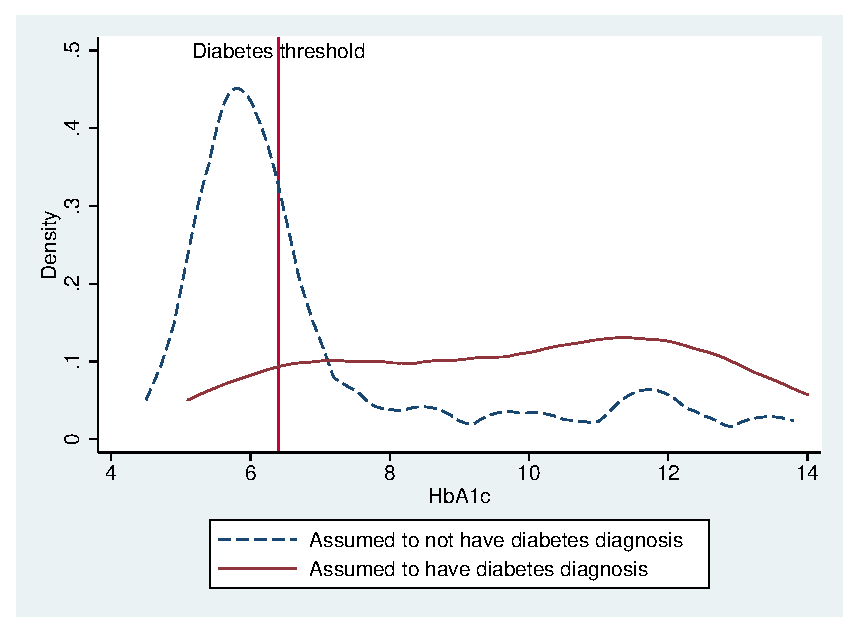
\includegraphics[width=.7\linewidth]{figures/kdensity_hba1c_inconsist.eps}\\
	\end{center}
\end{figure}


\clearpage

\subsection*{\DIFdelbegin \DIFdel{Early }\DIFdelend \DIFaddbegin \DIFadd{Early- }\DIFaddend versus \DIFdelbegin \DIFdel{late onset }\DIFdelend \DIFaddbegin \DIFadd{late-onset }\DIFaddend of diabetes}

\begin{table}[!ht]
	\caption{\label{tab:Labour_outcomes_earlylate}{\bf Labour outcomes and self-reported diabetes by diabetes onset.}}
	\begin{center}
		\begin{adjustbox}{max width=\linewidth} 
			\begin{threeparttable} 
				{
					\def\sym#1{\ifmmode^{#1}\else\(^{#1}\)\fi}
					\begin{tabular}{l*{6}{S S}}
						\toprule
						&\multicolumn{2}{c}{Employment}    &\multicolumn{2}{c}{Weekly working hours} &\multicolumn{2}{c}{Log hourly wages}  \\\cmidrule(lr){2-3}\cmidrule(lr){4-5}\cmidrule(lr){6-7}
						&\multicolumn{1}{c}{Males}&\multicolumn{1}{c}{Females}&\multicolumn{1}{c}{Males}&\multicolumn{1}{c}{Females}&\multicolumn{1}{c}{Males}&\multicolumn{1}{c}{Females}\\
						\midrule
						\DIFdelbeginFL \DIFdelFL{Early onset}\DIFdelendFL \DIFaddbeginFL \DIFaddFL{Early-onset    }\DIFaddendFL &    \DIFdelbeginFL \DIFdelFL{0.133         }\DIFdelendFL \DIFaddbeginFL \DIFaddFL{0.134         }\DIFaddendFL &   \DIFdelbeginFL \DIFdelFL{-0.206}\DIFdelendFL \DIFaddbeginFL \DIFaddFL{-0.195}\DIFaddendFL \sym{**} &   \DIFdelbeginFL \DIFdelFL{14.856}\DIFdelendFL \DIFaddbeginFL \DIFaddFL{14.395}\DIFaddendFL \sym{*}  &  \DIFdelbeginFL \DIFdelFL{-18.250}\DIFdelendFL \DIFaddbeginFL \DIFaddFL{-18.665}\DIFaddendFL \sym{*}  &   \DIFdelbeginFL \DIFdelFL{-0.490         }\DIFdelendFL \DIFaddbeginFL \DIFaddFL{-0.513}\sym{*}  \DIFaddendFL &    \DIFdelbeginFL \DIFdelFL{0.375}\DIFdelendFL \DIFaddbeginFL \DIFaddFL{0.362}\DIFaddendFL \sym{***}\\
						&  (0.176)         &  (0.086)         &  (\DIFdelbeginFL \DIFdelFL{8.329}\DIFdelendFL \DIFaddbeginFL \DIFaddFL{8.377}\DIFaddendFL )         &  (\DIFdelbeginFL \DIFdelFL{9.515}\DIFdelendFL \DIFaddbeginFL \DIFaddFL{9.650}\DIFaddendFL )         &  (\DIFdelbeginFL \DIFdelFL{0.337}\DIFdelendFL \DIFaddbeginFL \DIFaddFL{0.311}\DIFaddendFL )         &  (\DIFdelbeginFL \DIFdelFL{0.057}\DIFdelendFL \DIFaddbeginFL \DIFaddFL{0.039}\DIFaddendFL )         \\
						\DIFdelbeginFL \DIFdelFL{Late onset}\DIFdelendFL \DIFaddbeginFL \DIFaddFL{Late-onset    }\DIFaddendFL &   \DIFdelbeginFL \DIFdelFL{-0.059}%DIFDELCMD < \sym{**} %%%
\DIFdelendFL \DIFaddbeginFL \DIFaddFL{-0.082}\sym{***}\DIFaddendFL &   \DIFdelbeginFL \DIFdelFL{-0.047}%DIFDELCMD < \sym{*}  %%%
\DIFdelendFL \DIFaddbeginFL \DIFaddFL{-0.053}\sym{**} \DIFaddendFL &   \DIFdelbeginFL \DIFdelFL{-0.936         }\DIFdelendFL \DIFaddbeginFL \DIFaddFL{-1.360         }\DIFaddendFL &   \DIFdelbeginFL \DIFdelFL{-1.346         }\DIFdelendFL \DIFaddbeginFL \DIFaddFL{-1.267         }\DIFaddendFL &    \DIFdelbeginFL \DIFdelFL{0.071         }\DIFdelendFL \DIFaddbeginFL \DIFaddFL{0.016         }\DIFaddendFL &    \DIFdelbeginFL \DIFdelFL{0.074         }\DIFdelendFL \DIFaddbeginFL \DIFaddFL{0.059         }\DIFaddendFL \\
						&  (\DIFdelbeginFL \DIFdelFL{0.026}\DIFdelendFL \DIFaddbeginFL \DIFaddFL{0.025}\DIFaddendFL )         &  (0.025)         &  (\DIFdelbeginFL \DIFdelFL{1.510}\DIFdelendFL \DIFaddbeginFL \DIFaddFL{1.500}\DIFaddendFL )         &  (\DIFdelbeginFL \DIFdelFL{2.553}\DIFdelendFL \DIFaddbeginFL \DIFaddFL{2.565}\DIFaddendFL )         &  (\DIFdelbeginFL \DIFdelFL{0.068}\DIFdelendFL \DIFaddbeginFL \DIFaddFL{0.067}\DIFaddendFL )         &  (\DIFdelbeginFL \DIFdelFL{0.161}\DIFdelendFL \DIFaddbeginFL \DIFaddFL{0.165}\DIFaddendFL )         \\
						\DIFdelbeginFL %DIFDELCMD < 

%DIFDELCMD < 						%%%
\DIFdelendFL \midrule
						N         &   21388         &    27339         &    \DIFdelbeginFL \DIFdelFL{13828         }\DIFdelendFL \DIFaddbeginFL \DIFaddFL{17618         }\DIFaddendFL &     \DIFdelbeginFL \DIFdelFL{7068         }\DIFdelendFL \DIFaddbeginFL \DIFaddFL{9115         }\DIFaddendFL &    \DIFdelbeginFL \DIFdelFL{17616         }\DIFdelendFL \DIFaddbeginFL \DIFaddFL{13830         }\DIFaddendFL &     \DIFdelbeginFL \DIFdelFL{9112         }\DIFdelendFL \DIFaddbeginFL \DIFaddFL{7070         }\DIFaddendFL \\
						\bottomrule
					\end{tabular}
					\begin{tablenotes}
						\item \footnotesize \textit{Notes} Robust standard errors in parentheses. All models include \DIFdelbeginFL \DIFdelFL{variables for  states, urbanization, level of education, marital status, number of children < 6, wealth, health insurance status, age squared and one dummy variable for each calendar year }\DIFdelendFL \DIFaddbeginFL \DIFaddFL{calendar year dummies}\DIFaddendFL . \sym{*} \(p<0.10\), \sym{**} \(p<0.05\), \sym{***} \(p<0.01\).
					\end{tablenotes}
				}
			\end{threeparttable}
		\end{adjustbox}
	\end{center}
\end{table} 
\clearpage

\begin{table}[p]
	\caption{\label{tab:Worktype_earlylate}{\bf Selection into types of work and self-reported diabetes by diabetes onset.}}
	\begin{center}
		\begin{adjustbox}{max width=\linewidth} 
			\begin{threeparttable} 
				{
					\def\sym#1{\ifmmode^{#1}\else\(^{#1}\)\fi}
					\begin{tabular}{l*{6}{S S}}
						\toprule
						&\multicolumn{2}{c}{Non-agric.}       &\multicolumn{2}{c}{Agriculture}      &\multicolumn{2}{c}{Self-employed}    \\\cmidrule(lr){2-3}\cmidrule(lr){4-5}\cmidrule(lr){6-7}
						&\multicolumn{1}{c}{Males}&\multicolumn{1}{c}{Females}&\multicolumn{1}{c}{Males}&\multicolumn{1}{c}{Females}&\multicolumn{1}{c}{Males}&\multicolumn{1}{c}{Females}\\
						\midrule
						\DIFdelbeginFL \DIFdelFL{Early onset }\DIFdelendFL \DIFaddbeginFL \DIFaddFL{Early-onset}\DIFaddendFL &    \DIFdelbeginFL \DIFdelFL{0.030         }\DIFdelendFL \DIFaddbeginFL \DIFaddFL{0.036         }\DIFaddendFL &   -0.105         &   \DIFdelbeginFL \DIFdelFL{-0.226         }\DIFdelendFL \DIFaddbeginFL \DIFaddFL{-0.233}\sym{*}  \DIFaddendFL &   \DIFdelbeginFL \DIFdelFL{-0.068         }\DIFdelendFL \DIFaddbeginFL \DIFaddFL{-0.066         }\DIFaddendFL &    0.328\sym{**} &   \DIFdelbeginFL \DIFdelFL{-0.027         }\DIFdelendFL \DIFaddbeginFL \DIFaddFL{-0.020         }\DIFaddendFL \\
						&  (\DIFdelbeginFL \DIFdelFL{0.216}\DIFdelendFL \DIFaddbeginFL \DIFaddFL{0.215}\DIFaddendFL )         &  (0.074)         &  (0.139)         &  (0.047)         &  (0.161)         &  (\DIFdelbeginFL \DIFdelFL{0.048}\DIFdelendFL \DIFaddbeginFL \DIFaddFL{0.049}\DIFaddendFL )         \\
						\DIFdelbeginFL \DIFdelFL{Late onset }\DIFdelendFL \DIFaddbeginFL \DIFaddFL{Late-onset}\DIFaddendFL &   \DIFdelbeginFL \DIFdelFL{-0.007         }\DIFdelendFL \DIFaddbeginFL \DIFaddFL{-0.024         }\DIFaddendFL &    \DIFdelbeginFL \DIFdelFL{0.007         }\DIFdelendFL \DIFaddbeginFL \DIFaddFL{0.006         }\DIFaddendFL &   \DIFdelbeginFL \DIFdelFL{-0.001         }\DIFdelendFL \DIFaddbeginFL \DIFaddFL{-0.008         }\DIFaddendFL &   \DIFdelbeginFL \DIFdelFL{-0.018}\DIFdelendFL \DIFaddbeginFL \DIFaddFL{-0.019}\DIFaddendFL \sym{**} &   \DIFdelbeginFL \DIFdelFL{-0.054}\DIFdelendFL \DIFaddbeginFL \DIFaddFL{-0.056}\DIFaddendFL \sym{**} &   \DIFdelbeginFL \DIFdelFL{-0.029         }\DIFdelendFL \DIFaddbeginFL \DIFaddFL{-0.033}\sym{*}  \DIFaddendFL \\
						&  (0.029)         &  (0.019)         &  (0.022)         &  (0.009)         &  (0.026)         &  (0.019)         \\
						\midrule
						N         &\DIFdelbeginFL \DIFdelFL{20719         }\DIFdelendFL \DIFaddbeginFL \DIFaddFL{20537         }\DIFaddendFL &\DIFdelbeginFL \DIFdelFL{26575         }\DIFdelendFL \DIFaddbeginFL \DIFaddFL{26478         }\DIFaddendFL &\DIFdelbeginFL \DIFdelFL{20719         }\DIFdelendFL \DIFaddbeginFL \DIFaddFL{20537         }\DIFaddendFL &\DIFdelbeginFL \DIFdelFL{26575         }\DIFdelendFL \DIFaddbeginFL \DIFaddFL{26478         }\DIFaddendFL &\DIFdelbeginFL \DIFdelFL{20719         }\DIFdelendFL \DIFaddbeginFL \DIFaddFL{20537         }\DIFaddendFL &\DIFdelbeginFL \DIFdelFL{26575         }\DIFdelendFL \DIFaddbeginFL \DIFaddFL{26478         }\DIFaddendFL \\
						\bottomrule
					\end{tabular}
					\begin{tablenotes}
						\item \footnotesize \textit{Notes} Robust standard errors in parentheses. All models include \DIFdelbeginFL \DIFdelFL{variables for  states, urbanization, level of education, marital status, number of children < 6, wealth, health insurance status, age squared and one dummy variable for each calendar year }\DIFdelendFL \DIFaddbeginFL \DIFaddFL{calendar year dummies}\DIFaddendFL . \sym{*} \(p<0.10\), \sym{**} \(p<0.05\), \sym{***} \(p<0.01\).
					\end{tablenotes}
				}
			\end{threeparttable}
		\end{adjustbox}
	\end{center}
\end{table} 

\clearpage

\begin{table}[p]
	\caption{\label{tab:Self-reported-diabetes-duration_earlylate}{\bf Relationship between self-reported years since diagnosis and employment probabilities using continuous duration by diabetes onset.}}
	\begin{center}
		%\resizebox{\linewidth}{!}{%
		\begin{adjustbox}{max width=\linewidth}
			\begin{threeparttable}
				{
					\def\sym#1{\ifmmode^{#1}\else\(^{#1}\)\fi}
					\begin{tabular}{l*{6}{S S}}
						\toprule
						&\multicolumn{2}{c}{Employment}       &\DIFdelbeginFL %DIFDELCMD < \multicolumn{2}{c}{Monthly work hours} %%%
\DIFdelendFL \DIFaddbeginFL \multicolumn{2}{c}{Monthly working hours} \DIFaddendFL &\multicolumn{2}{c}{Log hourly wages} \\\cmidrule(lr){2-3}\cmidrule(lr){4-5}\cmidrule(lr){6-7}
						&\multicolumn{1}{c}{Males}&\multicolumn{1}{c}{Females}&\multicolumn{1}{c}{Males}&\multicolumn{1}{c}{Females}&\multicolumn{1}{c}{Males}&\multicolumn{1}{c}{Females}\\
						\midrule
						\DIFdelbeginFL \DIFdelFL{Early onset}\DIFdelendFL \DIFaddbeginFL \DIFaddFL{Survey year}\DIFaddendFL &    \DIFdelbeginFL \DIFdelFL{-0.005         }\DIFdelendFL \DIFaddbeginFL \DIFaddFL{0.003}\sym{***}\DIFaddendFL &    \DIFdelbeginFL \DIFdelFL{0.007         }\DIFdelendFL \DIFaddbeginFL \DIFaddFL{0.004}\sym{***}\DIFaddendFL &   \DIFaddbeginFL \DIFaddFL{-0.019         }\DIFaddendFL &    \DIFaddbeginFL \DIFaddFL{0.181}\sym{**} \DIFaddendFL &    \DIFaddbeginFL \DIFaddFL{0.014}\sym{***}\DIFaddendFL &    \DIFaddbeginFL \DIFaddFL{0.019}\sym{***}\DIFaddendFL \\
						&  (\DIFdelbeginFL \DIFdelFL{0.017}\DIFdelendFL \DIFaddbeginFL \DIFaddFL{0.001}\DIFaddendFL )         &  (\DIFdelbeginFL \DIFdelFL{0.013}\DIFdelendFL \DIFaddbeginFL \DIFaddFL{0.001}\DIFaddendFL )         &  \DIFaddbeginFL \DIFaddFL{(0.050)         }\DIFaddendFL &  \DIFaddbeginFL \DIFaddFL{(0.080)         }\DIFaddendFL &  \DIFaddbeginFL \DIFaddFL{(0.003)         }\DIFaddendFL &  \DIFaddbeginFL \DIFaddFL{(0.004)         }\DIFaddendFL \\
						\DIFdelbeginFL \DIFdelFL{Late onset}\DIFdelendFL \DIFaddbeginFL \DIFaddFL{Years since diagnosis at baseline (early-onset) $\times$ Survey year}\DIFaddendFL &    \DIFdelbeginFL \DIFdelFL{-0.012}%DIFDELCMD < \sym{**} %%%
\DIFdelendFL \DIFaddbeginFL \DIFaddFL{-0.003         }&    \DIFaddFL{0.001         }&    \DIFaddFL{0.197         }&   \DIFaddFL{-2.924}\sym{***}\DIFaddendFL &   -0.008         \DIFaddbeginFL &    \DIFaddFL{0.263}\sym{***}\\
						&  \DIFaddFL{(0.003)         }&  \DIFaddFL{(0.001)         }&  \DIFaddFL{(0.234)         }&  \DIFaddFL{(0.040)         }&  \DIFaddFL{(0.019)         }&  \DIFaddFL{(0.002)         }\\
						\DIFaddFL{Years since diagnosis at baseline (late-onset) $\times$ Survey year}&   \DIFaddFL{-0.003}\sym{***}&   \DIFaddFL{-0.001         }&    \DIFaddFL{0.007         }&    \DIFaddFL{0.042         }&   \DIFaddFL{-0.004         }&   \DIFaddFL{-0.010}\sym{***}\\
						&  \DIFaddFL{(0.001)         }&  \DIFaddFL{(0.001)         }&  \DIFaddFL{(0.062)         }&  \DIFaddFL{(0.104)         }&  \DIFaddFL{(0.003)         }&  \DIFaddFL{(0.002)         }\\
						\midrule
						\DIFaddFL{N         }&   \DIFaddFL{20760         }&    \DIFaddFL{26313         }&    \DIFaddFL{17137         }&     \DIFaddFL{8863         }&    \DIFaddFL{13481         }&     \DIFaddFL{6885         }\\
						\bottomrule
					\end{tabular}
					\begin{tablenotes}
						\item \footnotesize \textit{\DIFaddFL{Notes}}  \DIFaddFL{Robust standard errors in parentheses. }\sym{*} \DIFaddFL{\(p<0.10\), }\DIFaddendFL \sym{**} \DIFaddbeginFL \DIFaddFL{\(p<0.05\), }\sym{***} \DIFaddFL{\(p<0.01\).
					}\end{tablenotes}
				}
			\end{threeparttable}
		\end{adjustbox}
	\end{center}
\end{table}


\clearpage

\begin{table}[!ht]
	\caption{\label{tab:Biomarker_observations}{\bf Number of observations with diabetes (HbA1c $\geq 6.5\%$) and self-reported diabetes.}}
	\begin{center}
		\begin{adjustbox}{max width=\linewidth}
			\begin{threeparttable}
				{
					\def\sym#1{\ifmmode^{#1}\else\(^{#1}\)\fi}
					\begin{tabular}{lcccc}
						\toprule
						&\multicolumn{1}{c}{$HbA1c < 6.5\%$}&\multicolumn{1}{c}{HbA1c $\geq 6.5\%$}&\multicolumn{1}{c}{Total}\\
						\midrule
						No self-reported diabetes (N) & 4544 & 1181 & 5725 &  \\
						\hspace*{10mm}Row  \% & 79\% & 21\% & 100\% &  \\
						\hspace*{10mm}Cell \% & \textbf{71\%} & \textbf{18\%} & - & \\
						Self-reported diabetes (N) & 129 & 554 & 683 &  \\
						\hspace*{10mm}Row \%  & 19\% & 81\% & 100\% &  \\
						\hspace*{10mm}Cell \% & \textbf{2\%} &\textbf{9\%} &- & \\
						Total (N) & 4673 & 1735 & 6408 &  \\ 
						\bottomrule
					\end{tabular}
					\begin{tablenotes}
						\item
					\end{tablenotes}
				}
			\end{threeparttable}
		\end{adjustbox}
	\end{center}
\end{table}


\clearpage

\subsection*{\DIFadd{Robustness checks}}

\subsubsection*{\DIFadd{Additional time-variant controls}}

\begin{table}[p]
	\caption{\label{tab:Self-reported-diabetes-and_morecontrols)}{\bf Labour outcomes and self-reported diabetes including additional time-variant controls.}}
	\begin{center}
		\begin{adjustbox}{max width=\linewidth}
			\begin{threeparttable}
				{
					\def\sym#1{\ifmmode^{#1}\else\(^{#1}\)\fi}
					\begin{tabular}{l*{6}{S S}}
						\toprule
					&\multicolumn{2}{c}{Employment}       &\multicolumn{2}{c}{Monthly working hours} &\multicolumn{2}{c}{Log hourly wages} \\\cmidrule(lr){2-3}\cmidrule(lr){4-5}\cmidrule(lr){6-7}
					&\multicolumn{1}{c}{Males}&\multicolumn{1}{c}{Females}&\multicolumn{1}{c}{Males}&\multicolumn{1}{c}{Females}&\multicolumn{1}{c}{Males}&\multicolumn{1}{c}{Females}\\
					\midrule
						\DIFaddFL{Diabetes  }&   \DIFaddFL{-0.074}\sym{***}&   \DIFaddFL{-0.070}\DIFaddendFL \sym{***}\DIFaddbeginFL &   \DIFaddFL{-0.906         }&   \DIFaddFL{-2.170         }&    \DIFaddFL{0.021         }&    \DIFaddFL{0.071         }\DIFaddendFL \\
						&  (\DIFdelbeginFL \DIFdelFL{0.005}\DIFdelendFL \DIFaddbeginFL \DIFaddFL{0.025}\DIFaddendFL )         &  (\DIFdelbeginFL \DIFdelFL{0.004}\DIFdelendFL \DIFaddbeginFL \DIFaddFL{0.024}\DIFaddendFL )         &  (\DIFdelbeginFL \DIFdelFL{0.275}\DIFdelendFL \DIFaddbeginFL \DIFaddFL{1.496}\DIFaddendFL )         &  (\DIFdelbeginFL \DIFdelFL{0.505}\DIFdelendFL \DIFaddbeginFL \DIFaddFL{2.515}\DIFaddendFL )         &  (\DIFdelbeginFL \DIFdelFL{0.013}\DIFdelendFL \DIFaddbeginFL \DIFaddFL{0.066)         }&  \DIFaddFL{(0.157)         }\\
						\midrule
						\DIFaddFL{N         }&    \DIFaddFL{21388         }&    \DIFaddFL{27339         }&    \DIFaddFL{17618         }&     \DIFaddFL{9115         }&    \DIFaddFL{13830         }&     \DIFaddFL{7070         }\\
						\bottomrule
					\end{tabular}
					\begin{tablenotes}
						\item \footnotesize \textit{\DIFaddFL{Notes}} \DIFaddFL{Robust standard errors in parentheses. All models include variables for  states, urbanization, level of education, marital status, number of children < 6, wealth, health insurance status, and one dummy variable for each calendar year. }\sym{*} \DIFaddFL{\(p<0.10\), }\sym{**} \DIFaddFL{\(p<0.05\), }\sym{***} \DIFaddFL{\(p<0.01\). \(p<0.01\).
					}\end{tablenotes}
				}
			\end{threeparttable}
		\end{adjustbox}
	\end{center}
\end{table} 
\clearpage

\begin{table}[p]
	\caption{\label{tab:Self-reported-diabetes-selection_morecontrols}{\bf Selection into types of work and self-reported diabetes including additional time-variant controls.}}
	\begin{center}
		%DIF > \resizebox{\linewidth}{!}{%
		\begin{adjustbox}{max width=\linewidth}
			\begin{threeparttable}
				{
						\def\sym#1{\ifmmode^{#1}\else\(^{#1}\)\fi}
					\begin{tabular}{l*{6}{S S}}
						\toprule
					&\multicolumn{3}{c}{Males}                               &\multicolumn{3}{c}{Females}                             \\\cmidrule(lr){2-4}\cmidrule(lr){5-7}
					&\multicolumn{1}{c}{Non-agric.}&\multicolumn{1}{c}{Agric.}&\multicolumn{1}{c}{Self-employed}&\multicolumn{1}{c}{Non-agric.}&\multicolumn{1}{c}{Agric.}&\multicolumn{1}{c}{Self-employed}\\
						\midrule
						\DIFaddFL{Diabetes  }&   \DIFaddFL{-0.018         }&   \DIFaddFL{-0.012         }&   \DIFaddFL{-0.048}\sym{*}  &   \DIFaddFL{-0.007         }&   \DIFaddFL{-0.023}\sym{***}&   \DIFaddFL{-0.033}\sym{*}  \\
						&  \DIFaddFL{(0.029}\DIFaddendFL )         &  (0.022)         \DIFaddbeginFL &  \DIFaddFL{(0.026)         }&  \DIFaddFL{(0.018)         }&  \DIFaddFL{(0.009)         }&  \DIFaddFL{(0.018)         }\DIFaddendFL \\
						\midrule
						N         &    \DIFdelbeginFL \DIFdelFL{16308         }\DIFdelendFL \DIFaddbeginFL \DIFaddFL{20537         }\DIFaddendFL &    \DIFdelbeginFL \DIFdelFL{22450         }\DIFdelendFL \DIFaddbeginFL \DIFaddFL{20537         }\DIFaddendFL &    \DIFdelbeginFL \DIFdelFL{13592         }\DIFdelendFL \DIFaddbeginFL \DIFaddFL{20537         }\DIFaddendFL &    \DIFdelbeginFL \DIFdelFL{7394         }\DIFdelendFL \DIFaddbeginFL \DIFaddFL{26478         }\DIFaddendFL &    \DIFdelbeginFL \DIFdelFL{10778         }\DIFdelendFL \DIFaddbeginFL \DIFaddFL{26478         }\DIFaddendFL &    \DIFdelbeginFL \DIFdelFL{5748         }\DIFdelendFL \DIFaddbeginFL \DIFaddFL{26478         }\DIFaddendFL \\
						\bottomrule
					\end{tabular}
					\begin{tablenotes}
						\item \footnotesize \textit{Notes} \DIFdelbeginFL \DIFdelFL{The effects of early onset diabetes on wages and working hours could not be estimated due to no within-variation for diabetes. }\DIFdelendFL Robust standard errors in parentheses. All models include variables for  states, urbanization, level of education, marital status, number of children < 6, wealth, health insurance status, \DIFdelbeginFL \DIFdelFL{age squared }\DIFdelendFL and one dummy variable for each calendar year. \sym{*} \(p<0.10\), \sym{**} \(p<0.05\), \sym{***} \(p<0.01\). \DIFaddbeginFL \DIFaddFL{\(p<0.01\).
					}\DIFaddendFL \end{tablenotes}
				}
			\end{threeparttable}
		\end{adjustbox}
	\end{center}
\end{table} 
\DIFdelbegin %DIFDELCMD < 

%DIFDELCMD < %%%
\DIFdelend \clearpage

\DIFdelbegin \subsection*{\DIFdel{Random effects model}}
%DIFAUXCMD
%DIFDELCMD < 

%DIFDELCMD < \begin{table}[!ht]
%DIFDELCMD < 	%%%
\DIFdelendFL \DIFaddbeginFL \begin{table}[p]
	\DIFaddendFL \caption{\DIFdelbeginFL %DIFDELCMD < \label{tab:Self-reported-diabetes-duration_RE}{\bf Relationship between self-reported years since diagnosis and employment probabilities using continuous duration and duration splines (random effects).}%%%
\DIFdelendFL \DIFaddbeginFL \label{tab:Self-reported-diabetes-duration_morecontrols}{\bf Relationship between self-reported years since diagnosis and employment probabilities using continuous duration and duration splines including additional time-variant controls.}\DIFaddendFL }
	\begin{center}
		%\resizebox{\linewidth}{!}{%
		\DIFdelbeginFL %DIFDELCMD < \begin{adjustbox}{max width=\linewidth}
%DIFDELCMD < 			%%%
\DIFdelendFL \DIFaddbeginFL \begin{adjustbox}{max width=.9\linewidth}
			\DIFaddendFL \begin{threeparttable}
				{
					\def\sym#1{\ifmmode^{#1}\else\(^{#1}\)\fi}
					\begin{tabular}{l*{6}{S S}}
						\toprule
						&\multicolumn{2}{c}{Employment}       &\DIFdelbeginFL %DIFDELCMD < \multicolumn{2}{c}{Weekly work hours}%%%
\DIFdelendFL \DIFaddbeginFL \multicolumn{2}{c}{Weekly working hours}\DIFaddendFL &\multicolumn{2}{c}{Log hourly wages} \\\cmidrule(lr){2-3}\cmidrule(lr){4-5}\cmidrule(lr){6-7}
						&\multicolumn{1}{c}{Males}&\multicolumn{1}{c}{Females}&\multicolumn{1}{c}{Males}&\multicolumn{1}{c}{Females}&\multicolumn{1}{c}{Males}&\multicolumn{1}{c}{Females}\\
						\midrule
						\textit{\textbf{Panel A: linear effect}} &&&&&&\\
						\DIFaddbeginFL \DIFaddFL{Survey year     }&    \DIFaddFL{0.002}\sym{***}&    \DIFaddFL{0.004}\sym{***}&   \DIFaddFL{-0.021         }&    \DIFaddFL{0.198}\sym{**} &    \DIFaddFL{0.014}\sym{***}&    \DIFaddFL{0.023}\sym{***}\\
						&  \DIFaddFL{(0.001)         }&  \DIFaddFL{(0.001)         }&  \DIFaddFL{(0.051)         }&  \DIFaddFL{(0.089)         }&  \DIFaddFL{(0.003)         }&  \DIFaddFL{(0.005)         }\\
						\DIFaddendFL Years since diagnosis \DIFaddbeginFL \DIFaddFL{at baseline $\times$ Survey year}\DIFaddendFL &  \DIFdelbeginFL \DIFdelFL{-0.007}\DIFdelendFL \DIFaddbeginFL \DIFaddFL{- -0.003}\DIFaddendFL \sym{***}&   \DIFdelbeginFL \DIFdelFL{-0.004}%DIFDELCMD < \sym{***}%%%
\DIFdelendFL \DIFaddbeginFL \DIFaddFL{-0.001}\sym{*}  \DIFaddendFL &    \DIFdelbeginFL \DIFdelFL{0.039         }\DIFdelendFL \DIFaddbeginFL \DIFaddFL{0.010         }\DIFaddendFL &    \DIFdelbeginFL \DIFdelFL{-0.130         }\DIFdelendFL \DIFaddbeginFL \DIFaddFL{0.030         }\DIFaddendFL &   \DIFdelbeginFL \DIFdelFL{0.010}%DIFDELCMD < \sym{**} %%%
\DIFdelendFL \DIFaddbeginFL \DIFaddFL{-0.004         }\DIFaddendFL &   -0.009\DIFaddbeginFL \sym{***}\DIFaddendFL \\
						&  (\DIFdelbeginFL \DIFdelFL{0.002}\DIFdelendFL \DIFaddbeginFL \DIFaddFL{0.001}\DIFaddendFL )         &  (0.001)         &  (\DIFdelbeginFL \DIFdelFL{0.102}\DIFdelendFL \DIFaddbeginFL \DIFaddFL{0.062}\DIFaddendFL )         &  (\DIFdelbeginFL \DIFdelFL{0.127}\DIFdelendFL \DIFaddbeginFL \DIFaddFL{0.103}\DIFaddendFL )         &  (\DIFdelbeginFL \DIFdelFL{0.005}\DIFdelendFL \DIFaddbeginFL \DIFaddFL{0.003}\DIFaddendFL )         &  (\DIFdelbeginFL \DIFdelFL{0.008}\DIFdelendFL \DIFaddbeginFL \DIFaddFL{0.003}\DIFaddendFL )         \\
						\textit{\textbf{Panel B: splines}} &&&&&&\\
						\DIFdelbeginFL \DIFdelFL{Years since SR diagnosis  }\DIFdelendFL \DIFaddbeginFL \DIFaddFL{Survey year     }&  \DIFaddFL{0.002}\sym{***}&    \DIFaddFL{0.004}\sym{***}&   \DIFaddFL{-0.017         }&    \DIFaddFL{0.198}\sym{**} \DIFaddendFL &    \DIFaddbeginFL \DIFaddFL{0.014}\sym{***}\DIFaddendFL &    \DIFaddbeginFL \DIFaddFL{0.024}\sym{***}\\
						\DIFaddendFL &  \DIFaddbeginFL \DIFaddFL{(0.001)         }\DIFaddendFL &  \DIFaddbeginFL \DIFaddFL{(0.001)         }&  \DIFaddFL{(0.051)         }\DIFaddendFL &  \DIFaddbeginFL \DIFaddFL{(0.090)         }&  \DIFaddFL{(0.003)         }\DIFaddendFL &  \DIFaddbeginFL \DIFaddFL{(0.005)         }\DIFaddendFL \\
						\DIFaddbeginFL \DIFaddFL{Interaction: Years since diagnosis at baseline with survey year }&\DIFaddendFL &&&&&\\
						\DIFaddbeginFL \DIFaddFL{\hspace*{10mm}}\DIFaddendFL 0--3&   \DIFdelbeginFL \DIFdelFL{-0.008         }\DIFdelendFL \DIFaddbeginFL \DIFaddFL{-0.006}\sym{*}  \DIFaddendFL &   \DIFdelbeginFL \DIFdelFL{-0.015}%DIFDELCMD < \sym{**} %%%
\DIFdelendFL \DIFaddbeginFL \DIFaddFL{-0.000         }\DIFaddendFL &   \DIFdelbeginFL \DIFdelFL{-0.035         }\DIFdelendFL \DIFaddbeginFL \DIFaddFL{-0.048         }\DIFaddendFL &    \DIFdelbeginFL \DIFdelFL{0.507         }\DIFdelendFL \DIFaddbeginFL \DIFaddFL{0.249         }\DIFaddendFL &   \DIFdelbeginFL \DIFdelFL{0.038}%DIFDELCMD < \sym{**} %%%
\DIFdelendFL \DIFaddbeginFL \DIFaddFL{-0.003         }\DIFaddendFL &   \DIFdelbeginFL \DIFdelFL{0.034         }\DIFdelendFL \DIFaddbeginFL \DIFaddFL{-0.033}\sym{**} \DIFaddendFL \\
						&  (\DIFdelbeginFL \DIFdelFL{0.006}\DIFdelendFL \DIFaddbeginFL \DIFaddFL{0.004}\DIFaddendFL )         &  (\DIFdelbeginFL \DIFdelFL{0.006}\DIFdelendFL \DIFaddbeginFL \DIFaddFL{0.003}\DIFaddendFL )         &  (\DIFdelbeginFL \DIFdelFL{0.346}\DIFdelendFL \DIFaddbeginFL \DIFaddFL{0.206}\DIFaddendFL )         &  (\DIFdelbeginFL \DIFdelFL{0.614}\DIFdelendFL \DIFaddbeginFL \DIFaddFL{0.237}\DIFaddendFL )         &  (\DIFdelbeginFL \DIFdelFL{0.017}\DIFdelendFL \DIFaddbeginFL \DIFaddFL{0.013}\DIFaddendFL )         &  (\DIFdelbeginFL \DIFdelFL{0.029}\DIFdelendFL \DIFaddbeginFL \DIFaddFL{0.014}\DIFaddendFL )         \\
						\DIFaddbeginFL \DIFaddFL{\hspace*{10mm}}\DIFaddendFL 4--7 &   \DIFdelbeginFL \DIFdelFL{0.001         }\DIFdelendFL \DIFaddbeginFL \DIFaddFL{0.006         }\DIFaddendFL &   \DIFdelbeginFL \DIFdelFL{0.004         }\DIFdelendFL \DIFaddbeginFL \DIFaddFL{-0.003         }\DIFaddendFL &   \DIFdelbeginFL \DIFdelFL{0.242         }\DIFdelendFL \DIFaddbeginFL \DIFaddFL{-0.301         }\DIFaddendFL &   \DIFdelbeginFL \DIFdelFL{-0.570         }\DIFdelendFL \DIFaddbeginFL \DIFaddFL{-0.274         }\DIFaddendFL &   \DIFdelbeginFL \DIFdelFL{-0.032         }\DIFdelendFL \DIFaddbeginFL \DIFaddFL{-0.022         }\DIFaddendFL &    \DIFdelbeginFL \DIFdelFL{-0.048         }\DIFdelendFL \DIFaddbeginFL \DIFaddFL{0.018         }\DIFaddendFL \\
						&  (\DIFdelbeginFL \DIFdelFL{0.011}\DIFdelendFL \DIFaddbeginFL \DIFaddFL{0.008}\DIFaddendFL )         &  (\DIFdelbeginFL \DIFdelFL{0.011}\DIFdelendFL \DIFaddbeginFL \DIFaddFL{0.004}\DIFaddendFL )         &  (\DIFdelbeginFL \DIFdelFL{0.665}\DIFdelendFL \DIFaddbeginFL \DIFaddFL{0.468}\DIFaddendFL )         &  (\DIFdelbeginFL \DIFdelFL{1.062}\DIFdelendFL \DIFaddbeginFL \DIFaddFL{0.467}\DIFaddendFL )         &  (\DIFdelbeginFL \DIFdelFL{0.032}\DIFdelendFL \DIFaddbeginFL \DIFaddFL{0.023}\DIFaddendFL )         &  (\DIFdelbeginFL \DIFdelFL{0.052}\DIFdelendFL \DIFaddbeginFL \DIFaddFL{0.024}\DIFaddendFL )         \\
						\DIFaddbeginFL \DIFaddFL{\hspace*{10mm}}\DIFaddendFL 8--12 &  \DIFdelbeginFL \DIFdelFL{-0.008         }\DIFdelendFL \DIFaddbeginFL \DIFaddFL{-0.015}\sym{*}  \DIFaddendFL &   \DIFdelbeginFL \DIFdelFL{0.002         }\DIFdelendFL \DIFaddbeginFL \DIFaddFL{-0.003         }\DIFaddendFL &    \DIFdelbeginFL \DIFdelFL{-0.116         }\DIFdelendFL \DIFaddbeginFL \DIFaddFL{0.406         }\DIFaddendFL &   \DIFdelbeginFL \DIFdelFL{-0.080         }\DIFdelendFL \DIFaddbeginFL \DIFaddFL{-0.973         }\DIFaddendFL &    \DIFdelbeginFL \DIFdelFL{-0.003         }\DIFdelendFL \DIFaddbeginFL \DIFaddFL{0.047}\sym{*}  \DIFaddendFL &    \DIFdelbeginFL \DIFdelFL{-0.074         }\DIFdelendFL \DIFaddbeginFL \DIFaddFL{0.021         }\DIFaddendFL \\
						&  (\DIFdelbeginFL \DIFdelFL{0.015}\DIFdelendFL \DIFaddbeginFL \DIFaddFL{0.009}\DIFaddendFL )         &  (\DIFdelbeginFL \DIFdelFL{0.011}\DIFdelendFL \DIFaddbeginFL \DIFaddFL{0.005}\DIFaddendFL )         &  (\DIFdelbeginFL \DIFdelFL{0.855}\DIFdelendFL \DIFaddbeginFL \DIFaddFL{0.518}\DIFaddendFL )         &  (\DIFdelbeginFL \DIFdelFL{1.098}\DIFdelendFL \DIFaddbeginFL \DIFaddFL{0.724}\DIFaddendFL )         &  (\DIFdelbeginFL \DIFdelFL{0.041}\DIFdelendFL \DIFaddbeginFL \DIFaddFL{0.027}\DIFaddendFL )         &  (\DIFdelbeginFL \DIFdelFL{0.050}\DIFdelendFL \DIFaddbeginFL \DIFaddFL{0.040}\DIFaddendFL )         \\
						\DIFaddbeginFL \DIFaddFL{\hspace*{10mm}}\DIFaddendFL 13+ &    \DIFdelbeginFL \DIFdelFL{-0.012         }\DIFdelendFL \DIFaddbeginFL \DIFaddFL{0.003         }\DIFaddendFL &    \DIFdelbeginFL \DIFdelFL{-0.004         }\DIFdelendFL \DIFaddbeginFL \DIFaddFL{0.001         }\DIFaddendFL &    \DIFdelbeginFL \DIFdelFL{0.035         }\DIFdelendFL \DIFaddbeginFL \DIFaddFL{0.185         }\DIFaddendFL &    \DIFdelbeginFL \DIFdelFL{-0.339         }\DIFdelendFL \DIFaddbeginFL \DIFaddFL{2.080}\sym{***}\DIFaddendFL &   \DIFdelbeginFL \DIFdelFL{0.029         }\DIFdelendFL \DIFaddbeginFL \DIFaddFL{-0.026}\sym{**} \DIFaddendFL &   \DIFdelbeginFL \DIFdelFL{0.011         }\DIFdelendFL \DIFaddbeginFL \DIFaddFL{-0.043         }\DIFaddendFL \\
						&  (\DIFdelbeginFL \DIFdelFL{0.008}\DIFdelendFL \DIFaddbeginFL \DIFaddFL{0.002}\DIFaddendFL )         &  (\DIFdelbeginFL \DIFdelFL{0.003}\DIFdelendFL \DIFaddbeginFL \DIFaddFL{0.001}\DIFaddendFL )         &  (\DIFdelbeginFL \DIFdelFL{0.410}\DIFdelendFL \DIFaddbeginFL \DIFaddFL{0.212}\DIFaddendFL )         &  (\DIFdelbeginFL \DIFdelFL{0.241}\DIFdelendFL \DIFaddbeginFL \DIFaddFL{0.713}\DIFaddendFL )         &  (\DIFdelbeginFL \DIFdelFL{0.018}\DIFdelendFL \DIFaddbeginFL \DIFaddFL{0.012}\DIFaddendFL )         &  (\DIFdelbeginFL \DIFdelFL{0.017}\DIFdelendFL \DIFaddbeginFL \DIFaddFL{0.037}\DIFaddendFL )         \\
						\textit{\textbf{Panel C: dummies}} &&&&&&\\
						\DIFdelbeginFL \DIFdelFL{0--3}\DIFdelendFL \DIFaddbeginFL \DIFaddFL{Survey year     }\DIFaddendFL &    \DIFdelbeginFL \DIFdelFL{-0.036}%DIFDELCMD < \sym{*}  %%%
\DIFdelendFL \DIFaddbeginFL \DIFaddFL{0.002}\sym{***}\DIFaddendFL &    \DIFdelbeginFL \DIFdelFL{-0.041}\DIFdelendFL \DIFaddbeginFL \DIFaddFL{0.004}\sym{***}&   \DIFaddFL{-0.015         }&    \DIFaddFL{0.198}\DIFaddendFL \sym{**} &    \DIFdelbeginFL \DIFdelFL{-0.821         }\DIFdelendFL \DIFaddbeginFL \DIFaddFL{0.014}\sym{***}\DIFaddendFL &    \DIFdelbeginFL \DIFdelFL{1.091         }\DIFdelendFL \DIFaddbeginFL \DIFaddFL{0.024}\sym{***}\\
						\DIFaddendFL &  \DIFdelbeginFL \DIFdelFL{0.134}\DIFdelendFL \DIFaddbeginFL \DIFaddFL{(0.001)         }&  \DIFaddFL{(0.001)         }&  \DIFaddFL{(0.051)         }&  \DIFaddFL{(0.090)         }&  \DIFaddFL{(0.003)         }&  \DIFaddFL{(0.005)         }\\
						\DIFaddFL{Interaction: Years since diagnosis at baseline with survey year }&&&&&&\\
						\DIFaddFL{\hspace*{10mm}0--3}&    \DIFaddFL{-0.024}\DIFaddendFL \sym{**} &   \DIFdelbeginFL \DIFdelFL{0.021         }\DIFdelendFL \DIFaddbeginFL \DIFaddFL{-0.009         }&   \DIFaddFL{-0.256         }&    \DIFaddFL{0.218         }&   \DIFaddFL{-0.033         }&   \DIFaddFL{-0.078}\sym{*}  \DIFaddendFL \\
						&  (\DIFdelbeginFL \DIFdelFL{0.021}\DIFdelendFL \DIFaddbeginFL \DIFaddFL{0.011}\DIFaddendFL )         &  (\DIFdelbeginFL \DIFdelFL{0.021}\DIFdelendFL \DIFaddbeginFL \DIFaddFL{0.009}\DIFaddendFL )         &  (\DIFdelbeginFL \DIFdelFL{1.154}\DIFdelendFL \DIFaddbeginFL \DIFaddFL{0.667}\DIFaddendFL )         &  (\DIFdelbeginFL \DIFdelFL{1.826}\DIFdelendFL \DIFaddbeginFL \DIFaddFL{0.618}\DIFaddendFL )         &  (\DIFdelbeginFL \DIFdelFL{0.054}\DIFdelendFL \DIFaddbeginFL \DIFaddFL{0.040}\DIFaddendFL )         &  (\DIFdelbeginFL \DIFdelFL{0.083}\DIFdelendFL \DIFaddbeginFL \DIFaddFL{0.044}\DIFaddendFL )         \\
						\DIFaddbeginFL \DIFaddFL{\hspace*{10mm}}\DIFaddendFL 4--7 &  \DIFdelbeginFL \DIFdelFL{-0.014         }\DIFdelendFL \DIFaddbeginFL \DIFaddFL{-0.017         }\DIFaddendFL &    \DIFdelbeginFL \DIFdelFL{-0.056}%DIFDELCMD < \sym{**} %%%
\DIFdelendFL \DIFaddbeginFL \DIFaddFL{0.001         }\DIFaddendFL &   \DIFdelbeginFL \DIFdelFL{0.877         }\DIFdelendFL \DIFaddbeginFL \DIFaddFL{-1.190         }\DIFaddendFL &    \DIFdelbeginFL \DIFdelFL{1.200         }\DIFdelendFL \DIFaddbeginFL \DIFaddFL{0.617         }\DIFaddendFL &   \DIFdelbeginFL \DIFdelFL{0.093         }\DIFdelendFL \DIFaddbeginFL \DIFaddFL{-0.034         }\DIFaddendFL &   \DIFdelbeginFL \DIFdelFL{-0.003         }\DIFdelendFL \DIFaddbeginFL \DIFaddFL{-0.072         }\DIFaddendFL \\
						&  (\DIFdelbeginFL \DIFdelFL{0.022}\DIFdelendFL \DIFaddbeginFL \DIFaddFL{0.016}\DIFaddendFL )         &  (\DIFdelbeginFL \DIFdelFL{0.023}\DIFdelendFL \DIFaddbeginFL \DIFaddFL{0.009}\DIFaddendFL )         &  (\DIFdelbeginFL \DIFdelFL{1.375}\DIFdelendFL \DIFaddbeginFL \DIFaddFL{0.769}\DIFaddendFL )         &  (\DIFdelbeginFL \DIFdelFL{2.530}\DIFdelendFL \DIFaddbeginFL \DIFaddFL{1.177}\DIFaddendFL )         &  (\DIFdelbeginFL \DIFdelFL{0.059}\DIFdelendFL \DIFaddbeginFL \DIFaddFL{0.047}\DIFaddendFL )         &  (\DIFdelbeginFL \DIFdelFL{0.118}\DIFdelendFL \DIFaddbeginFL \DIFaddFL{0.047}\DIFaddendFL )         \\
						\DIFaddbeginFL \DIFaddFL{\hspace*{10mm}}\DIFaddendFL 8--12 &    \DIFdelbeginFL \DIFdelFL{-0.069}%DIFDELCMD < \sym{*}  %%%
\DIFdelendFL \DIFaddbeginFL \DIFaddFL{-0.030         }\DIFaddendFL &   \DIFdelbeginFL \DIFdelFL{-0.043         }\DIFdelendFL \DIFaddbeginFL \DIFaddFL{-0.047}\sym{***}\DIFaddendFL &   \DIFdelbeginFL \DIFdelFL{0.427         }\DIFdelendFL \DIFaddbeginFL \DIFaddFL{-0.462         }\DIFaddendFL &   \DIFdelbeginFL \DIFdelFL{0.302         }\DIFdelendFL \DIFaddbeginFL \DIFaddFL{-3.305}\sym{*}  \DIFaddendFL &    \DIFdelbeginFL \DIFdelFL{-0.070         }\DIFdelendFL \DIFaddbeginFL \DIFaddFL{0.052         }\DIFaddendFL &   \DIFdelbeginFL \DIFdelFL{-0.148         }\DIFdelendFL \DIFaddbeginFL \DIFaddFL{-0.011         }\DIFaddendFL \\
						&  (\DIFdelbeginFL \DIFdelFL{0.037}\DIFdelendFL \DIFaddbeginFL \DIFaddFL{0.020}\DIFaddendFL )         &  (\DIFdelbeginFL \DIFdelFL{0.030}\DIFdelendFL \DIFaddbeginFL \DIFaddFL{0.012}\DIFaddendFL )         &  (\DIFdelbeginFL \DIFdelFL{2.288}\DIFdelendFL \DIFaddbeginFL \DIFaddFL{1.174}\DIFaddendFL )         &  (\DIFdelbeginFL \DIFdelFL{2.995}\DIFdelendFL \DIFaddbeginFL \DIFaddFL{1.840}\DIFaddendFL )         &  (\DIFdelbeginFL \DIFdelFL{0.101}\DIFdelendFL \DIFaddbeginFL \DIFaddFL{0.071}\DIFaddendFL )         &  (\DIFdelbeginFL \DIFdelFL{0.117}\DIFdelendFL \DIFaddbeginFL \DIFaddFL{0.115}\DIFaddendFL )         \\
						\DIFaddbeginFL \DIFaddFL{\hspace*{10mm}}\DIFaddendFL 13+ &   \DIFdelbeginFL \DIFdelFL{-0.121}%DIFDELCMD < \sym{***}%%%
\DIFdelendFL \DIFaddbeginFL \DIFaddFL{-0.042}\sym{**} \DIFaddendFL &   \DIFdelbeginFL \DIFdelFL{-0.043         }\DIFdelendFL \DIFaddbeginFL \DIFaddFL{-0.010         }\DIFaddendFL &    \DIFdelbeginFL \DIFdelFL{-0.568         }\DIFdelendFL \DIFaddbeginFL \DIFaddFL{1.757         }\DIFaddendFL &    \DIFdelbeginFL \DIFdelFL{-2.104         }\DIFdelendFL \DIFaddbeginFL \DIFaddFL{1.305         }\DIFaddendFL &   \DIFdelbeginFL \DIFdelFL{0.242}%DIFDELCMD < \sym{*}  %%%
\DIFdelendFL \DIFaddbeginFL \DIFaddFL{-0.156}\sym{**} \DIFaddendFL &   \DIFdelbeginFL \DIFdelFL{-0.279}%DIFDELCMD < \sym{*}  %%%
\DIFdelendFL \DIFaddbeginFL \DIFaddFL{-0.131}\sym{***}\DIFaddendFL \\
						&  (\DIFdelbeginFL \DIFdelFL{0.045}\DIFdelendFL \DIFaddbeginFL \DIFaddFL{0.021}\DIFaddendFL )         &  (\DIFdelbeginFL \DIFdelFL{0.031}\DIFdelendFL \DIFaddbeginFL \DIFaddFL{0.014}\DIFaddendFL )         &  (\DIFdelbeginFL \DIFdelFL{2.280}\DIFdelendFL \DIFaddbeginFL \DIFaddFL{1.431}\DIFaddendFL )         &  (\DIFdelbeginFL \DIFdelFL{3.088}\DIFdelendFL \DIFaddbeginFL \DIFaddFL{2.071}\DIFaddendFL )         &  (\DIFdelbeginFL \DIFdelFL{0.126}\DIFdelendFL \DIFaddbeginFL \DIFaddFL{0.067}\DIFaddendFL )         &  (\DIFdelbeginFL \DIFdelFL{0.153}\DIFdelendFL \DIFaddbeginFL \DIFaddFL{0.020}\DIFaddendFL )         \\
						\midrule
						N               &    \DIFdelbeginFL \DIFdelFL{16308         }\DIFdelendFL \DIFaddbeginFL \DIFaddFL{20760         }\DIFaddendFL &    \DIFdelbeginFL \DIFdelFL{22450         }\DIFdelendFL \DIFaddbeginFL \DIFaddFL{26313         }\DIFaddendFL &    \DIFdelbeginFL \DIFdelFL{13592         }\DIFdelendFL \DIFaddbeginFL \DIFaddFL{17137         }\DIFaddendFL &     \DIFdelbeginFL \DIFdelFL{7394         }\DIFdelendFL \DIFaddbeginFL \DIFaddFL{8863         }\DIFaddendFL &    \DIFdelbeginFL \DIFdelFL{10778         }\DIFdelendFL \DIFaddbeginFL \DIFaddFL{13481         }\DIFaddendFL &     \DIFdelbeginFL \DIFdelFL{5748         }\DIFdelendFL \DIFaddbeginFL \DIFaddFL{6885         }\DIFaddendFL \\
						\bottomrule
					\end{tabular}
					\begin{tablenotes}
					\item \footnotesize \textit{Notes} \DIFdelbeginFL \DIFdelFL{Panel A presents the results of the linear specifications. Panel B presents the results of the non-linear specifications. }\DIFdelendFL Robust standard errors in parentheses. All models include variables for  states, urbanization, level of education, marital status, number of children < 6, wealth \DIFdelbeginFL \DIFdelFL{, }\DIFdelendFL \DIFaddbeginFL \DIFaddFL{and }\DIFaddendFL health insurance status\DIFdelbeginFL \DIFdelFL{, age squared and one dummy variable for each calendar year}\DIFdelendFL . \sym{*} \(p<0.10\), \sym{**} \(p<0.05\), \sym{***} \(p<0.01\). \DIFaddbeginFL \DIFaddFL{\(p<0.01\).
					}\DIFaddendFL \end{tablenotes}
				}
			\end{threeparttable}
		\end{adjustbox}
	\end{center}
\end{table}
 \DIFaddbegin \subsubsection*{\DIFadd{Additionally controlling for time-variant controls and obesity}}
\DIFaddend 


\begin{table}[!ht]
	\caption{\DIFdelbeginFL %DIFDELCMD < \label{tab:Self-reported-diabetes-and_obesity}{\bf Labour outcomes and self-reported diabetes controlling for obesity}%%%
\DIFdelendFL \DIFaddbeginFL \label{tab:Self-reported-diabetes-and_obesity}{\bf Labour outcomes and self-reported diabetes controlling for obesity. }\DIFaddendFL }
	\begin{center}
		\begin{adjustbox}{max width=\linewidth}
			\begin{threeparttable}
				{
					\def\sym#1{\ifmmode^{#1}\else\(^{#1}\)\fi}
					\begin{tabular}{l*{6}{S S}}
						\toprule
						&\multicolumn{2}{c}{Employment}       &\DIFdelbeginFL %DIFDELCMD < \multicolumn{2}{c}{Weekly work hours}%%%
\DIFdelendFL \DIFaddbeginFL \multicolumn{2}{c}{Weekly working hours}\DIFaddendFL &\multicolumn{2}{c}{Log hourly wages} \\\cmidrule(lr){2-3}\cmidrule(lr){4-5}\cmidrule(lr){6-7}
						&\multicolumn{1}{c}{Males}&\multicolumn{1}{c}{Females}&\multicolumn{1}{c}{Males}&\multicolumn{1}{c}{Females}&\multicolumn{1}{c}{Males}&\multicolumn{1}{c}{Females}\\
						\midrule
					Obese (BMI $\geq 30$)&    \DIFdelbeginFL \DIFdelFL{0.007         }\DIFdelendFL \DIFaddbeginFL \DIFaddFL{0.009         }\DIFaddendFL &   \DIFdelbeginFL \DIFdelFL{-0.005         }\DIFdelendFL \DIFaddbeginFL \DIFaddFL{-0.002         }\DIFaddendFL &   \DIFdelbeginFL \DIFdelFL{-0.127         }\DIFdelendFL \DIFaddbeginFL \DIFaddFL{-0.025         }\DIFaddendFL &   \DIFdelbeginFL \DIFdelFL{-1.144         }\DIFdelendFL \DIFaddbeginFL \DIFaddFL{-1.079         }\DIFaddendFL &    \DIFdelbeginFL \DIFdelFL{0.018         }\DIFdelendFL \DIFaddbeginFL \DIFaddFL{0.027         }\DIFaddendFL &    \DIFdelbeginFL \DIFdelFL{0.082         }\DIFdelendFL \DIFaddbeginFL \DIFaddFL{0.081         }\DIFaddendFL \\
					&  (0.012)         &  (0.013)         &  (\DIFdelbeginFL \DIFdelFL{0.773}\DIFdelendFL \DIFaddbeginFL \DIFaddFL{0.771}\DIFaddendFL )         &  (\DIFdelbeginFL \DIFdelFL{1.188}\DIFdelendFL \DIFaddbeginFL \DIFaddFL{1.184}\DIFaddendFL )         &  (0.038)         &  (0.061)         \\
					Diabetes  &   \DIFdelbeginFL \DIFdelFL{-0.046         }%DIFDELCMD < &   %%%
\DIFdelFL{-0.064}\DIFdelendFL \DIFaddbeginFL \DIFaddFL{-0.065}\DIFaddendFL \sym{**} &   \DIFdelbeginFL \DIFdelFL{-0.689         }\DIFdelendFL \DIFaddbeginFL \DIFaddFL{-0.078}\sym{***}\DIFaddendFL &   \DIFdelbeginFL \DIFdelFL{-0.169         }\DIFdelendFL \DIFaddbeginFL \DIFaddFL{-1.097         }\DIFaddendFL &   \DIFdelbeginFL \DIFdelFL{0.036         }\DIFdelendFL \DIFaddbeginFL \DIFaddFL{-0.291         }\DIFaddendFL &    \DIFdelbeginFL \DIFdelFL{0.033         }\DIFdelendFL \DIFaddbeginFL \DIFaddFL{0.001         }&    \DIFaddFL{0.037         }\DIFaddendFL \\
					&  (0.028)         &  (0.027)         &  (\DIFdelbeginFL \DIFdelFL{1.772}\DIFdelendFL \DIFaddbeginFL \DIFaddFL{1.768}\DIFaddendFL )         &  (\DIFdelbeginFL \DIFdelFL{2.904}\DIFdelendFL \DIFaddbeginFL \DIFaddFL{2.909}\DIFaddendFL )         &  (\DIFdelbeginFL \DIFdelFL{0.078}\DIFdelendFL \DIFaddbeginFL \DIFaddFL{0.076}\DIFaddendFL )         &  (\DIFdelbeginFL \DIFdelFL{0.183}\DIFdelendFL \DIFaddbeginFL \DIFaddFL{0.181}\DIFaddendFL )         \\
					\midrule
					N         &    17992         &    24145         &    \DIFdelbeginFL \DIFdelFL{14866         }\DIFdelendFL \DIFaddbeginFL \DIFaddFL{14867         }\DIFaddendFL &     \DIFdelbeginFL \DIFdelFL{7929         }\DIFdelendFL \DIFaddbeginFL \DIFaddFL{7931         }\DIFaddendFL &    \DIFdelbeginFL \DIFdelFL{11711         }\DIFdelendFL \DIFaddbeginFL \DIFaddFL{11712         }\DIFaddendFL &     \DIFdelbeginFL \DIFdelFL{6166         }\DIFdelendFL \DIFaddbeginFL \DIFaddFL{6167         }\DIFaddendFL \\
						\bottomrule
					\end{tabular}
					\begin{tablenotes}
						\item \footnotesize \textit{Notes} Robust standard errors in parentheses. All models include variables for  states, urbanization, level of education, marital status, number of children < 6, wealth, health insurance status, \DIFdelbeginFL \DIFdelFL{age squared }\DIFdelendFL and one dummy variable for each calendar year. \sym{*} \(p<0.10\), \sym{**} \(p<0.05\), \sym{***} \(p<0.01\).
					\end{tablenotes}
				}
			\end{threeparttable}
		\end{adjustbox}
	\end{center}
\end{table} 

\begin{table}[!ht]
	\caption{\label{tab:Self-reported-diabetes-selection_WB_obese}{\bf Selection into types of work and self-reported diabetes controlling for obesity.}}
	\begin{center}
		%\resizebox{\linewidth}{!}{%
		\begin{adjustbox}{max width=\linewidth}
			\begin{threeparttable}
				{
					\def\sym#1{\ifmmode^{#1}\else\(^{#1}\)\fi}
					\begin{tabular}{l*{6}{S S}}
						\toprule
						&\multicolumn{3}{c}{Males}                               &\multicolumn{3}{c}{Females}                             \\\cmidrule(lr){2-4}\cmidrule(lr){5-7}
						&\multicolumn{1}{c}{Non-agric.}&\multicolumn{1}{c}{Agric.}&\multicolumn{1}{c}{Self-employed}&\multicolumn{1}{c}{Non-agric.}&\multicolumn{1}{c}{Agric.}&\multicolumn{1}{c}{Self-employed}\\
						\midrule
						Obese (BMI $\geq 30$)&    \DIFdelbeginFL \DIFdelFL{0.005         }\DIFdelendFL \DIFaddbeginFL \DIFaddFL{0.007         }\DIFaddendFL &   \DIFdelbeginFL \DIFdelFL{-0.032}\DIFdelendFL \DIFaddbeginFL \DIFaddFL{-0.031}\DIFaddendFL \sym{**} &    \DIFdelbeginFL \DIFdelFL{0.036}%DIFDELCMD < \sym{***}%%%
\DIFdelendFL \DIFaddbeginFL \DIFaddFL{0.035}\sym{**} \DIFaddendFL &   \DIFdelbeginFL \DIFdelFL{-0.021}\DIFdelendFL \DIFaddbeginFL \DIFaddFL{-0.019}\DIFaddendFL \sym{*}  &    \DIFdelbeginFL \DIFdelFL{0.003         }\DIFdelendFL \DIFaddbeginFL \DIFaddFL{0.002         }\DIFaddendFL &    \DIFdelbeginFL \DIFdelFL{0.010         }\DIFdelendFL \DIFaddbeginFL \DIFaddFL{0.011         }\DIFaddendFL \\
						&  (0.017)         &  (0.013)         &  (0.014)         &  (0.011)         &  (0.004)         &  (0.009)         \\
						Diabetes  &    \DIFdelbeginFL \DIFdelFL{0.010         }\DIFdelendFL \DIFaddbeginFL \DIFaddFL{0.001         }\DIFaddendFL &   \DIFdelbeginFL \DIFdelFL{0.002         }\DIFdelendFL \DIFaddbeginFL \DIFaddFL{-0.001         }\DIFaddendFL &   \DIFdelbeginFL \DIFdelFL{-0.060}\DIFdelendFL \DIFaddbeginFL \DIFaddFL{-0.067}\DIFaddendFL \sym{**} &   \DIFdelbeginFL \DIFdelFL{-0.011         }\DIFdelendFL \DIFaddbeginFL \DIFaddFL{-0.018         }\DIFaddendFL &   \DIFdelbeginFL \DIFdelFL{-0.020}\DIFdelendFL \DIFaddbeginFL \DIFaddFL{-0.023}\DIFaddendFL \sym{**} &   \DIFdelbeginFL \DIFdelFL{-0.025         }\DIFdelendFL \DIFaddbeginFL \DIFaddFL{-0.030         }\DIFaddendFL \\
						&  (\DIFdelbeginFL \DIFdelFL{0.033}\DIFdelendFL \DIFaddbeginFL \DIFaddFL{0.034}\DIFaddendFL )         &  (0.023)         &  (0.028)         &  (0.020)         &  (0.010)         &  (0.021)         \\
						\midrule
						N         &    \DIFdelbeginFL \DIFdelFL{17414         }\DIFdelendFL \DIFaddbeginFL \DIFaddFL{17261         }\DIFaddendFL &    \DIFdelbeginFL \DIFdelFL{17414         }\DIFdelendFL \DIFaddbeginFL \DIFaddFL{17261         }\DIFaddendFL &    \DIFdelbeginFL \DIFdelFL{17414         }\DIFdelendFL \DIFaddbeginFL \DIFaddFL{17261         }\DIFaddendFL &    \DIFdelbeginFL \DIFdelFL{23458         }\DIFdelendFL \DIFaddbeginFL \DIFaddFL{23377         }\DIFaddendFL &    \DIFdelbeginFL \DIFdelFL{23458         }\DIFdelendFL \DIFaddbeginFL \DIFaddFL{23377         }\DIFaddendFL &    \DIFdelbeginFL \DIFdelFL{23458         }\DIFdelendFL \DIFaddbeginFL \DIFaddFL{23377         }\DIFaddendFL \\
						\bottomrule
					\end{tabular}
					\begin{tablenotes}
						\item \footnotesize \textit{Notes} Robust standard errors in parentheses. All models include variables for  states, urbanization, level of education, marital status, number of children < 6, wealth, health insurance status, \DIFdelbeginFL \DIFdelFL{age squared }\DIFdelendFL and one dummy variable for each calendar year. \sym{*} \(p<0.10\), \sym{**} \(p<0.05\), \sym{***} \(p<0.01\).
					\end{tablenotes}
				}
			\end{threeparttable}
		\end{adjustbox}
	\end{center}
\end{table} 

\begin{table}[!ht]
	\caption{\label{tab:Self-reported-diabetes-duration_obese}{\bf Relationship between self-reported years since diagnosis and employment probabilities using continuous duration and duration splines and controlling for obesity.}}
	\begin{center}
		%\resizebox{\linewidth}{!}{%
		\begin{adjustbox}{max width=.9\linewidth}
			\begin{threeparttable}
				{
					\def\sym#1{\ifmmode^{#1}\else\(^{#1}\)\fi}
					\begin{tabular}{l*{6}{S S}}
						\toprule
						&\multicolumn{2}{c}{Employment}       &\DIFdelbeginFL %DIFDELCMD < \multicolumn{2}{c}{Weekly work hours}%%%
\DIFdelendFL \DIFaddbeginFL \multicolumn{2}{c}{Weekly working hours}\DIFaddendFL &\multicolumn{2}{c}{Log hourly wages} \\\cmidrule(lr){2-3}\cmidrule(lr){4-5}\cmidrule(lr){6-7}
						&\multicolumn{1}{c}{Males}&\multicolumn{1}{c}{Females}&\multicolumn{1}{c}{Males}&\multicolumn{1}{c}{Females}&\multicolumn{1}{c}{Males}&\multicolumn{1}{c}{Females}\\
						\midrule
						\textit{\textbf{Panel A: linear effect}} &&&&&&\\
						Obese (BMI $\geq 30$)&    \DIFdelbeginFL \DIFdelFL{0.003         }\DIFdelendFL \DIFaddbeginFL \DIFaddFL{0.011         }\DIFaddendFL &   \DIFdelbeginFL \DIFdelFL{-0.010         }\DIFdelendFL \DIFaddbeginFL \DIFaddFL{-0.003         }\DIFaddendFL &   \DIFdelbeginFL \DIFdelFL{0.059         }\DIFdelendFL \DIFaddbeginFL \DIFaddFL{-0.249         }\DIFaddendFL &   \DIFdelbeginFL \DIFdelFL{-0.412         }\DIFdelendFL \DIFaddbeginFL \DIFaddFL{-0.914         }\DIFaddendFL &    \DIFdelbeginFL \DIFdelFL{0.026         }\DIFdelendFL \DIFaddbeginFL \DIFaddFL{0.024         }\DIFaddendFL &    \DIFdelbeginFL \DIFdelFL{0.035         }\DIFdelendFL \DIFaddbeginFL \DIFaddFL{0.058         }\DIFaddendFL \\
						&  (0.012)         &  (0.014)         &  (\DIFdelbeginFL \DIFdelFL{0.831}\DIFdelendFL \DIFaddbeginFL \DIFaddFL{0.791}\DIFaddendFL )         &  (\DIFdelbeginFL \DIFdelFL{1.247}\DIFdelendFL \DIFaddbeginFL \DIFaddFL{1.222}\DIFaddendFL )         &  (0.040)         &  (\DIFdelbeginFL \DIFdelFL{0.064}\DIFdelendFL \DIFaddbeginFL \DIFaddFL{0.063)         }\\
						\DIFaddFL{Survey year     }&    \DIFaddFL{0.002}\sym{*}  &    \DIFaddFL{0.004}\sym{***}&   \DIFaddFL{-0.039         }&    \DIFaddFL{0.182}\sym{*}  &    \DIFaddFL{0.014}\sym{***}&    \DIFaddFL{0.020}\sym{***}\\
						&  \DIFaddFL{(0.001)         }&  \DIFaddFL{(0.001)         }&  \DIFaddFL{(0.060)         }&  \DIFaddFL{(0.103)         }&  \DIFaddFL{(0.003)         }&  \DIFaddFL{(0.006}\DIFaddendFL )         \\
						Years since diagnosis \DIFaddbeginFL \DIFaddFL{at baseline $\times$ Survey year}\DIFaddendFL &   \DIFdelbeginFL \DIFdelFL{-0.019}\DIFdelendFL \DIFaddbeginFL \DIFaddFL{-0.004}\DIFaddendFL \sym{***}&   \DIFdelbeginFL \DIFdelFL{-0.008         }\DIFdelendFL \DIFaddbeginFL \DIFaddFL{-0.001}\sym{*}  \DIFaddendFL &    \DIFdelbeginFL \DIFdelFL{0.259         }\DIFdelendFL \DIFaddbeginFL \DIFaddFL{0.039         }\DIFaddendFL &   \DIFdelbeginFL \DIFdelFL{-0.008         }\DIFdelendFL \DIFaddbeginFL \DIFaddFL{-0.023         }\DIFaddendFL &   \DIFdelbeginFL \DIFdelFL{-0.016         }\DIFdelendFL \DIFaddbeginFL \DIFaddFL{-0.004         }\DIFaddendFL &   \DIFdelbeginFL \DIFdelFL{-0.073}\DIFdelendFL \DIFaddbeginFL \DIFaddFL{-0.011}\DIFaddendFL \sym{**} \\
						&  (\DIFdelbeginFL \DIFdelFL{0.006}\DIFdelendFL \DIFaddbeginFL \DIFaddFL{0.001}\DIFaddendFL )         &  (\DIFdelbeginFL \DIFdelFL{0.006}\DIFdelendFL \DIFaddbeginFL \DIFaddFL{0.001}\DIFaddendFL )         &  (\DIFdelbeginFL \DIFdelFL{0.375}\DIFdelendFL \DIFaddbeginFL \DIFaddFL{0.064}\DIFaddendFL )         &  (\DIFdelbeginFL \DIFdelFL{0.721}\DIFdelendFL \DIFaddbeginFL \DIFaddFL{0.092}\DIFaddendFL )         &  (\DIFdelbeginFL \DIFdelFL{0.019}\DIFdelendFL \DIFaddbeginFL \DIFaddFL{0.003}\DIFaddendFL )         &  (\DIFdelbeginFL \DIFdelFL{0.034}\DIFdelendFL \DIFaddbeginFL \DIFaddFL{0.005}\DIFaddendFL )         \\
						\textit{\textbf{Panel B: splines}} &&&&&&\\
						Years since SR diagnosis  &&&&&&\\
						Obese (BMI $\geq 30$)&    \DIFdelbeginFL \DIFdelFL{0.003         }\DIFdelendFL \DIFaddbeginFL \DIFaddFL{0.011         }\DIFaddendFL &   \DIFdelbeginFL \DIFdelFL{-0.009         }\DIFdelendFL \DIFaddbeginFL \DIFaddFL{-0.002         }\DIFaddendFL &   \DIFdelbeginFL \DIFdelFL{0.073         }\DIFdelendFL \DIFaddbeginFL \DIFaddFL{-0.221         }\DIFaddendFL &   \DIFdelbeginFL \DIFdelFL{-0.371         }\DIFdelendFL \DIFaddbeginFL \DIFaddFL{-0.898         }\DIFaddendFL &    \DIFdelbeginFL \DIFdelFL{0.027         }\DIFdelendFL \DIFaddbeginFL \DIFaddFL{0.025         }\DIFaddendFL &    \DIFdelbeginFL \DIFdelFL{0.036         }\DIFdelendFL \DIFaddbeginFL \DIFaddFL{0.055         }\DIFaddendFL \\
						&  (\DIFdelbeginFL \DIFdelFL{0.013}\DIFdelendFL \DIFaddbeginFL \DIFaddFL{0.012}\DIFaddendFL )         &  (0.014)         &  (\DIFdelbeginFL \DIFdelFL{0.832}\DIFdelendFL \DIFaddbeginFL \DIFaddFL{0.785}\DIFaddendFL )         &  (\DIFdelbeginFL \DIFdelFL{1.247}\DIFdelendFL \DIFaddbeginFL \DIFaddFL{1.225}\DIFaddendFL )         &  (0.040)         &  (\DIFdelbeginFL \DIFdelFL{0.064}\DIFdelendFL \DIFaddbeginFL \DIFaddFL{0.063)         }\\
						\DIFaddFL{Survey year     }&    \DIFaddFL{0.002}\sym{**} &    \DIFaddFL{0.004}\sym{***}&   \DIFaddFL{-0.037         }&    \DIFaddFL{0.178}\sym{*}  &    \DIFaddFL{0.014}\sym{***}&    \DIFaddFL{0.021}\sym{***}\\
						&  \DIFaddFL{(0.001)         }&  \DIFaddFL{(0.001)         }&  \DIFaddFL{(0.060)         }&  \DIFaddFL{(0.103)         }&  \DIFaddFL{(0.003)         }&  \DIFaddFL{(0.006}\DIFaddendFL )         \\
						0--3 &   \DIFdelbeginFL \DIFdelFL{-0.014         }\DIFdelendFL \DIFaddbeginFL \DIFaddFL{-0.008}\sym{*}  \DIFaddendFL &    \DIFdelbeginFL \DIFdelFL{-0.022         }\DIFdelendFL \DIFaddbeginFL \DIFaddFL{0.003         }\DIFaddendFL &    \DIFdelbeginFL \DIFdelFL{0.806         }\DIFdelendFL \DIFaddbeginFL \DIFaddFL{0.094         }\DIFaddendFL &    \DIFdelbeginFL \DIFdelFL{3.762         }\DIFdelendFL \DIFaddbeginFL \DIFaddFL{0.053         }\DIFaddendFL &   \DIFdelbeginFL \DIFdelFL{-0.070         }\DIFdelendFL \DIFaddbeginFL \DIFaddFL{-0.009         }\DIFaddendFL &   \DIFdelbeginFL \DIFdelFL{0.015         }\DIFdelendFL \DIFaddbeginFL \DIFaddFL{-0.033}\sym{**} \DIFaddendFL \\
						&  (\DIFdelbeginFL \DIFdelFL{0.015}\DIFdelendFL \DIFaddbeginFL \DIFaddFL{0.004}\DIFaddendFL )         &  (\DIFdelbeginFL \DIFdelFL{0.017}\DIFdelendFL \DIFaddbeginFL \DIFaddFL{0.003}\DIFaddendFL )         &  (\DIFdelbeginFL \DIFdelFL{1.051}\DIFdelendFL \DIFaddbeginFL \DIFaddFL{0.242}\DIFaddendFL )         &  (\DIFdelbeginFL \DIFdelFL{3.169}\DIFdelendFL \DIFaddbeginFL \DIFaddFL{0.212}\DIFaddendFL )         &  (\DIFdelbeginFL \DIFdelFL{0.057}\DIFdelendFL \DIFaddbeginFL \DIFaddFL{0.015}\DIFaddendFL )         &  (\DIFdelbeginFL \DIFdelFL{0.139}\DIFdelendFL \DIFaddbeginFL \DIFaddFL{0.014}\DIFaddendFL )         \\
						4--7 &    \DIFdelbeginFL \DIFdelFL{-0.003         }\DIFdelendFL \DIFaddbeginFL \DIFaddFL{0.000         }\DIFaddendFL &   \DIFdelbeginFL \DIFdelFL{0.009         }\DIFdelendFL \DIFaddbeginFL \DIFaddFL{-0.008         }\DIFaddendFL &   \DIFdelbeginFL \DIFdelFL{-0.293         }\DIFdelendFL \DIFaddbeginFL \DIFaddFL{-0.488         }\DIFaddendFL &    \DIFdelbeginFL \DIFdelFL{-3.921}%DIFDELCMD < \sym{**} %%%
\DIFdelendFL \DIFaddbeginFL \DIFaddFL{0.288         }\DIFaddendFL &   \DIFdelbeginFL \DIFdelFL{0.035         }\DIFdelendFL \DIFaddbeginFL \DIFaddFL{-0.002         }\DIFaddendFL &    \DIFdelbeginFL \DIFdelFL{-0.121         }\DIFdelendFL \DIFaddbeginFL \DIFaddFL{0.015         }\DIFaddendFL \\
						&  (\DIFdelbeginFL \DIFdelFL{0.018}\DIFdelendFL \DIFaddbeginFL \DIFaddFL{0.009}\DIFaddendFL )         &  (\DIFdelbeginFL \DIFdelFL{0.015}\DIFdelendFL \DIFaddbeginFL \DIFaddFL{0.005}\DIFaddendFL )         &  (\DIFdelbeginFL \DIFdelFL{0.914}\DIFdelendFL \DIFaddbeginFL \DIFaddFL{0.527}\DIFaddendFL )         &  (\DIFdelbeginFL \DIFdelFL{1.811}\DIFdelendFL \DIFaddbeginFL \DIFaddFL{0.434}\DIFaddendFL )         &  (\DIFdelbeginFL \DIFdelFL{0.044}\DIFdelendFL \DIFaddbeginFL \DIFaddFL{0.024}\DIFaddendFL )         &  (\DIFdelbeginFL \DIFdelFL{0.108}\DIFdelendFL \DIFaddbeginFL \DIFaddFL{0.026}\DIFaddendFL )         \\
						8--12 &   \DIFdelbeginFL \DIFdelFL{-0.023         }\DIFdelendFL \DIFaddbeginFL \DIFaddFL{-0.007         }\DIFaddendFL &   \DIFdelbeginFL \DIFdelFL{0.001         }\DIFdelendFL \DIFaddbeginFL \DIFaddFL{-0.003         }\DIFaddendFL &    \DIFdelbeginFL \DIFdelFL{-0.098         }\DIFdelendFL \DIFaddbeginFL \DIFaddFL{0.599         }\DIFaddendFL &   \DIFdelbeginFL \DIFdelFL{3.082}%DIFDELCMD < \sym{*}  %%%
\DIFdelendFL \DIFaddbeginFL \DIFaddFL{-1.090         }\DIFaddendFL &    \DIFdelbeginFL \DIFdelFL{-0.062         }\DIFdelendFL \DIFaddbeginFL \DIFaddFL{0.017         }\DIFaddendFL &    \DIFdelbeginFL \DIFdelFL{-0.085         }\DIFdelendFL \DIFaddbeginFL \DIFaddFL{0.028         }\DIFaddendFL \\
						&  (\DIFdelbeginFL \DIFdelFL{0.022}\DIFdelendFL \DIFaddbeginFL \DIFaddFL{0.010}\DIFaddendFL )         &  (\DIFdelbeginFL \DIFdelFL{0.016}\DIFdelendFL \DIFaddbeginFL \DIFaddFL{0.007}\DIFaddendFL )         &  (\DIFdelbeginFL \DIFdelFL{1.350}\DIFdelendFL \DIFaddbeginFL \DIFaddFL{0.541}\DIFaddendFL )         &  (\DIFdelbeginFL \DIFdelFL{1.736}\DIFdelendFL \DIFaddbeginFL \DIFaddFL{0.727}\DIFaddendFL )         &  (\DIFdelbeginFL \DIFdelFL{0.066}\DIFdelendFL \DIFaddbeginFL \DIFaddFL{0.021}\DIFaddendFL )         &  (\DIFdelbeginFL \DIFdelFL{0.074}\DIFdelendFL \DIFaddbeginFL \DIFaddFL{0.045}\DIFaddendFL )         \\
						13+ &    \DIFdelbeginFL \DIFdelFL{-0.038}%DIFDELCMD < \sym{**} %%%
\DIFdelendFL \DIFaddbeginFL \DIFaddFL{0.003         }\DIFaddendFL &    \DIFdelbeginFL \DIFdelFL{-0.024}%DIFDELCMD < \sym{*}  %%%
\DIFdelendFL \DIFaddbeginFL \DIFaddFL{0.000         }\DIFaddendFL &    \DIFdelbeginFL \DIFdelFL{0.855         }\DIFdelendFL \DIFaddbeginFL \DIFaddFL{0.135         }\DIFaddendFL &    \DIFdelbeginFL \DIFdelFL{-1.128         }\DIFdelendFL \DIFaddbeginFL \DIFaddFL{1.010         }\DIFaddendFL &   \DIFdelbeginFL \DIFdelFL{0.005         }\DIFdelendFL \DIFaddbeginFL \DIFaddFL{-0.017         }\DIFaddendFL &   \DIFdelbeginFL \DIFdelFL{-0.065         }\DIFdelendFL \DIFaddbeginFL \DIFaddFL{-0.066         }\DIFaddendFL \\
						&  (\DIFdelbeginFL \DIFdelFL{0.017}\DIFdelendFL \DIFaddbeginFL \DIFaddFL{0.005}\DIFaddendFL )         &  (\DIFdelbeginFL \DIFdelFL{0.012}\DIFdelendFL \DIFaddbeginFL \DIFaddFL{0.003}\DIFaddendFL )         &  (\DIFdelbeginFL \DIFdelFL{1.029}\DIFdelendFL \DIFaddbeginFL \DIFaddFL{0.179}\DIFaddendFL )         &  (\DIFdelbeginFL \DIFdelFL{1.421}\DIFdelendFL \DIFaddbeginFL \DIFaddFL{1.271}\DIFaddendFL )         &  (\DIFdelbeginFL \DIFdelFL{0.053}\DIFdelendFL \DIFaddbeginFL \DIFaddFL{0.011}\DIFaddendFL )         &  (\DIFdelbeginFL \DIFdelFL{0.063}\DIFdelendFL \DIFaddbeginFL \DIFaddFL{0.051}\DIFaddendFL )         \\
						\textit{\textbf{Panel C: dummies}} &&&&&&\\
						Obese (BMI \DIFdelbeginFL \DIFdelFL{$\geq 30$)}\DIFdelendFL \DIFaddbeginFL \DIFaddFL{$\geq 30)$}\DIFaddendFL &    \DIFdelbeginFL \DIFdelFL{0.005         }\DIFdelendFL \DIFaddbeginFL \DIFaddFL{0.011         }\DIFaddendFL &   \DIFdelbeginFL \DIFdelFL{-0.009         }\DIFdelendFL \DIFaddbeginFL \DIFaddFL{-0.003         }\DIFaddendFL &   \DIFdelbeginFL \DIFdelFL{0.044         }\DIFdelendFL \DIFaddbeginFL \DIFaddFL{-0.236         }\DIFaddendFL &   \DIFdelbeginFL \DIFdelFL{-0.378         }\DIFdelendFL \DIFaddbeginFL \DIFaddFL{-0.892         }\DIFaddendFL &    \DIFdelbeginFL \DIFdelFL{0.026         }\DIFdelendFL \DIFaddbeginFL \DIFaddFL{0.024         }\DIFaddendFL &    \DIFdelbeginFL \DIFdelFL{0.031         }\DIFdelendFL \DIFaddbeginFL \DIFaddFL{0.055         }\DIFaddendFL \\
						&  (0.012)         &  (0.014)         &  (\DIFdelbeginFL \DIFdelFL{0.831}\DIFdelendFL \DIFaddbeginFL \DIFaddFL{0.787}\DIFaddendFL )         &  (\DIFdelbeginFL \DIFdelFL{1.245}\DIFdelendFL \DIFaddbeginFL \DIFaddFL{1.223}\DIFaddendFL )         &  (0.040)         &  (\DIFdelbeginFL \DIFdelFL{0.064}\DIFdelendFL \DIFaddbeginFL \DIFaddFL{0.063}\DIFaddendFL )         \\
						\DIFdelbeginFL \DIFdelFL{0--3}\DIFdelendFL \DIFaddbeginFL \DIFaddFL{Survey year     }\DIFaddendFL &    \DIFdelbeginFL \DIFdelFL{0.028         }\DIFdelendFL \DIFaddbeginFL \DIFaddFL{0.002}\sym{**} \DIFaddendFL &    \DIFdelbeginFL \DIFdelFL{-0.032         }\DIFdelendFL \DIFaddbeginFL \DIFaddFL{0.004}\sym{***}\DIFaddendFL &   \DIFdelbeginFL \DIFdelFL{1.484         }\DIFdelendFL \DIFaddbeginFL \DIFaddFL{-0.035         }\DIFaddendFL &    \DIFdelbeginFL \DIFdelFL{22.434}\DIFdelendFL \DIFaddbeginFL \DIFaddFL{0.181}\DIFaddendFL \sym{*}  &    \DIFdelbeginFL \DIFdelFL{0.047         }\DIFdelendFL \DIFaddbeginFL \DIFaddFL{0.014}\sym{***}\DIFaddendFL &    \DIFdelbeginFL \DIFdelFL{-0.658         }\DIFdelendFL \DIFaddbeginFL \DIFaddFL{0.021}\sym{***}\DIFaddendFL \\
						&  (\DIFdelbeginFL \DIFdelFL{0.059}\DIFdelendFL \DIFaddbeginFL \DIFaddFL{0.001}\DIFaddendFL )         &  (\DIFdelbeginFL \DIFdelFL{0.065}\DIFdelendFL \DIFaddbeginFL \DIFaddFL{0.001}\DIFaddendFL )         &  (\DIFdelbeginFL \DIFdelFL{3.825}\DIFdelendFL \DIFaddbeginFL \DIFaddFL{0.060}\DIFaddendFL )         &  (\DIFdelbeginFL \DIFdelFL{11.579}\DIFdelendFL \DIFaddbeginFL \DIFaddFL{0.104}\DIFaddendFL )         &  (\DIFdelbeginFL \DIFdelFL{0.212}\DIFdelendFL \DIFaddbeginFL \DIFaddFL{0.003}\DIFaddendFL )         &  (\DIFdelbeginFL \DIFdelFL{0.622}\DIFdelendFL \DIFaddbeginFL \DIFaddFL{0.006}\DIFaddendFL )         \\
						\DIFdelbeginFL \DIFdelFL{4--7}\DIFdelendFL \DIFaddbeginFL \DIFaddFL{0--3}\DIFaddendFL &   \DIFdelbeginFL \DIFdelFL{0.001         }\DIFdelendFL \DIFaddbeginFL \DIFaddFL{-0.029}\sym{**} \DIFaddendFL &   \DIFdelbeginFL \DIFdelFL{-0.054         }\DIFdelendFL \DIFaddbeginFL \DIFaddFL{-0.001         }\DIFaddendFL &   \DIFdelbeginFL \DIFdelFL{2.399         }\DIFdelendFL \DIFaddbeginFL \DIFaddFL{-0.148         }\DIFaddendFL &   \DIFdelbeginFL \DIFdelFL{12.909         }\DIFdelendFL \DIFaddbeginFL \DIFaddFL{-0.326         }&   \DIFaddFL{-0.047         }&   \DIFaddFL{-0.083         }\\
						\DIFaddendFL &  \DIFaddbeginFL \DIFaddFL{(}\DIFaddendFL 0.013\DIFaddbeginFL \DIFaddFL{)         }\DIFaddendFL &  \DIFdelbeginFL \DIFdelFL{-0.793         }\DIFdelendFL \DIFaddbeginFL \DIFaddFL{(0.011)         }&  \DIFaddFL{(0.817)         }&  \DIFaddFL{(0.527)         }&  \DIFaddFL{(0.048)         }&  \DIFaddFL{(0.052)         }\\
						\DIFaddFL{4--7}&   \DIFaddFL{-0.034}\sym{*}  &    \DIFaddFL{0.004         }&   \DIFaddFL{-0.467         }&    \DIFaddFL{0.928         }&   \DIFaddFL{-0.046         }&   \DIFaddFL{-0.080}\sym{*}  \DIFaddendFL \\
						&  (\DIFdelbeginFL \DIFdelFL{0.044}\DIFdelendFL \DIFaddbeginFL \DIFaddFL{0.018}\DIFaddendFL )         &  (\DIFdelbeginFL \DIFdelFL{0.055}\DIFdelendFL \DIFaddbeginFL \DIFaddFL{0.011}\DIFaddendFL )         &  (\DIFdelbeginFL \DIFdelFL{3.181}\DIFdelendFL \DIFaddbeginFL \DIFaddFL{0.731}\DIFaddendFL )         &  (\DIFdelbeginFL \DIFdelFL{11.063}\DIFdelendFL \DIFaddbeginFL \DIFaddFL{1.195}\DIFaddendFL )         &  (\DIFdelbeginFL \DIFdelFL{0.154}\DIFdelendFL \DIFaddbeginFL \DIFaddFL{0.044}\DIFaddendFL )         &  (\DIFdelbeginFL \DIFdelFL{0.616}\DIFdelendFL \DIFaddbeginFL \DIFaddFL{0.049}\DIFaddendFL )         \\
						8--12&   \DIFdelbeginFL \DIFdelFL{-0.064         }\DIFdelendFL \DIFaddbeginFL \DIFaddFL{-0.048}\sym{**} \DIFaddendFL &   \DIFdelbeginFL \DIFdelFL{0.010         }\DIFdelendFL \DIFaddbeginFL \DIFaddFL{-0.062}\sym{***}\DIFaddendFL &   \DIFdelbeginFL \DIFdelFL{0.296         }\DIFdelendFL \DIFaddbeginFL \DIFaddFL{-0.831         }\DIFaddendFL &   \DIFdelbeginFL \DIFdelFL{15.604         }\DIFdelendFL \DIFaddbeginFL \DIFaddFL{-2.434         }\DIFaddendFL &    \DIFdelbeginFL \DIFdelFL{-0.293         }\DIFdelendFL \DIFaddbeginFL \DIFaddFL{0.043         }\DIFaddendFL &   \DIFdelbeginFL \DIFdelFL{-1.125}%DIFDELCMD < \sym{*}  %%%
\DIFdelendFL \DIFaddbeginFL \DIFaddFL{-0.000         }\DIFaddendFL \\
						&  (\DIFdelbeginFL \DIFdelFL{0.069}\DIFdelendFL \DIFaddbeginFL \DIFaddFL{0.020}\DIFaddendFL )         &  (\DIFdelbeginFL \DIFdelFL{0.066}\DIFdelendFL \DIFaddbeginFL \DIFaddFL{0.014}\DIFaddendFL )         &  (\DIFdelbeginFL \DIFdelFL{4.994}\DIFdelendFL \DIFaddbeginFL \DIFaddFL{1.426}\DIFaddendFL )         &  (\DIFdelbeginFL \DIFdelFL{11.038}\DIFdelendFL \DIFaddbeginFL \DIFaddFL{2.455}\DIFaddendFL )         &  (\DIFdelbeginFL \DIFdelFL{0.247}\DIFdelendFL \DIFaddbeginFL \DIFaddFL{0.050}\DIFaddendFL )         &  (\DIFdelbeginFL \DIFdelFL{0.583}\DIFdelendFL \DIFaddbeginFL \DIFaddFL{0.112}\DIFaddendFL )         \\
						13+& \DIFdelbeginFL \DIFdelFL{-0.208}%DIFDELCMD < \sym{**} %%%
\DIFdelendFL \DIFaddbeginFL \DIFaddFL{-0.032         }\DIFaddendFL &   \DIFdelbeginFL \DIFdelFL{-0.073         }\DIFdelendFL \DIFaddbeginFL \DIFaddFL{-0.018         }\DIFaddendFL &    \DIFdelbeginFL \DIFdelFL{-1.966         }\DIFdelendFL \DIFaddbeginFL \DIFaddFL{2.731}\sym{**} \DIFaddendFL &   \DIFdelbeginFL \DIFdelFL{17.459}%DIFDELCMD < \sym{*}  %%%
\DIFdelendFL \DIFaddbeginFL \DIFaddFL{-1.609}\sym{***}\DIFaddendFL &   \DIFdelbeginFL \DIFdelFL{0.168         }\DIFdelendFL \DIFaddbeginFL \DIFaddFL{-0.132}\sym{*}  \DIFaddendFL &   \DIFdelbeginFL \DIFdelFL{-1.090}%DIFDELCMD < \sym{**} %%%
\DIFdelendFL \DIFaddbeginFL \DIFaddFL{-0.159}\sym{***}\DIFaddendFL \\
						&  (\DIFdelbeginFL \DIFdelFL{0.105}\DIFdelendFL \DIFaddbeginFL \DIFaddFL{0.027}\DIFaddendFL )         &  (\DIFdelbeginFL \DIFdelFL{0.081}\DIFdelendFL \DIFaddbeginFL \DIFaddFL{0.017}\DIFaddendFL )         &  (\DIFdelbeginFL \DIFdelFL{4.975}\DIFdelendFL \DIFaddbeginFL \DIFaddFL{1.270}\DIFaddendFL )         &  (\DIFdelbeginFL \DIFdelFL{10.262}\DIFdelendFL \DIFaddbeginFL \DIFaddFL{0.507}\DIFaddendFL )         &  (\DIFdelbeginFL \DIFdelFL{0.256}\DIFdelendFL \DIFaddbeginFL \DIFaddFL{0.075}\DIFaddendFL )         &  (\DIFdelbeginFL \DIFdelFL{0.499}\DIFdelendFL \DIFaddbeginFL \DIFaddFL{0.016}\DIFaddendFL )         \\
						\midrule
						N               &    \DIFdelbeginFL \DIFdelFL{13912         }\DIFdelendFL \DIFaddbeginFL \DIFaddFL{17459         }\DIFaddendFL &    \DIFdelbeginFL \DIFdelFL{19972         }\DIFdelendFL \DIFaddbeginFL \DIFaddFL{23238         }\DIFaddendFL &    \DIFdelbeginFL \DIFdelFL{11622         }\DIFdelendFL \DIFaddbeginFL \DIFaddFL{14457         }\DIFaddendFL &     \DIFdelbeginFL \DIFdelFL{6487         }\DIFdelendFL \DIFaddbeginFL \DIFaddFL{7709         }\DIFaddendFL &    \DIFdelbeginFL \DIFdelFL{9262         }\DIFdelendFL \DIFaddbeginFL \DIFaddFL{11411         }\DIFaddendFL &     \DIFdelbeginFL \DIFdelFL{5054         }\DIFdelendFL \DIFaddbeginFL \DIFaddFL{6003         }\DIFaddendFL \\
						\bottomrule
					\end{tabular}
					\begin{tablenotes}
						\item \footnotesize \textit{Notes} Panel A presents the results of the linear specifications. Panel B presents the results of the non-linear specifications. Robust standard errors in parentheses. All models include variables for  states, urbanization, level of education, marital status, number of children < 6, wealth, health insurance status\DIFdelbeginFL \DIFdelFL{, age squared and one dummy variable for each calendar year}\DIFdelendFL . \sym{*} \(p<0.10\), \sym{**} \(p<0.05\), \sym{***} \(p<0.01\).
					\end{tablenotes}
				}
			\end{threeparttable}
		\end{adjustbox}
	\end{center}
\end{table}
\clearpage

\setcounter{table}{0} 
\DIFaddbegin \setcounter{page}{1}
\nolinenumbers
\DIFaddend \renewcommand{\thetable}{\arabic{table}}

\section*{Tables}

\begin{table}[!ht]
	\caption{\label{tab:Pooled-sample-characteristics}{\bf Descriptive statistics for the panel sample (2002,2005,2009).}}

	\begin{adjustbox}{max width=\linewidth, center}
		\begin{threeparttable}  %adds notes to tables
			{
				\def\sym#1{\ifmmode^{#1}\else\(^{#1}\)\fi}
				\begin{tabular}{l*{6}{S S}}
					\toprule
					&\multicolumn{3}{c}{Males}             &\multicolumn{3}{c}{Females}\\\cmidrule(lr){2-4}\cmidrule(lr){5-7}         
					&\multicolumn{1}{c}{No diabetes}&\multicolumn{1}{c}{Diabetes}&  \multicolumn{1}{c}{p (t-test)}&\multicolumn{1}{c}{No diabetes}&\multicolumn{1}{c}{Diabetes}&  \multicolumn{1}{c}{p (t-test)}\\
					\midrule
					\hspace*{10mm}\emph{Dependent variables} \\
					Employed            &        0.87&        0.80&        0.00&        0.37&        0.26&        0.00\\
					Hourly wage  (in Mexican Peso) &       42.29&       46.79&        0.83&       40.67&       36.33&        0.61\\
					Weekly working hours&       46.83&       46.51&        0.60&       39.06&       37.51&        0.09\\
					Non-agricultural worker or employee&        0.51&        0.41&        0.00&        0.24&        0.13&        0.00\\
					Agricultural worker&        0.19&        0.13&        0.00&        0.02&        0.01&        0.00\\
					Self-employed&        0.16&        0.26&        0.00&        0.09&        0.11&        0.04\\
					\hspace*{10mm}\emph{Diabetes variables} \\
					Diabetes duration (years)   &  &        \DIFdelbeginFL \DIFdelFL{7.40}\DIFdelendFL \DIFaddbeginFL \DIFaddFL{6.94 }\DIFaddendFL &        &        &        \DIFdelbeginFL \DIFdelFL{7.79}\DIFdelendFL \DIFaddbeginFL \DIFaddFL{7.09}\DIFaddendFL &        \\
					\hspace*{10mm}\emph{Control variables} \\
					Age                 &       35.31&       50.68&        0.00&       35.37&       50.45&        0.00\\
					Any medical insurance&        0.47&        0.59&        0.00&        0.50&        0.62&        0.00\\
					City of 2,5oo-15,000&        0.11&        0.09&        0.03&        0.11&        0.13&        0.00\\
					City of 15,000-100,000&        0.10&        0.14&        0.00&        0.10&        0.10&        0.40\\
					City of >100,000    &        0.34&        0.39&        0.00&        0.35&        0.34&        0.47\\
					Married             &        0.53&        0.77&        0.00&        0.53&        0.66&        0.00\\
					Number of children (age<6) in household&        1.49&        1.14&        0.00&        1.60&        1.13&        0.00\\
					Indigenous group    &        0.19&        0.15&        0.00&        0.19&        0.19&        0.86\\
					Education &&&&&& \\                    
					\hspace*{10mm}Secondary           &        0.31&        0.22&        0.00&        0.31&        0.16&        0.00\\
					\hspace*{10mm}High school         & 0.16&        0.07&        0.00&        0.14&        0.03&        0.00\\
					\hspace*{10mm}Higher education    & 0.11&        0.12&        0.39&        0.10&        0.03&        0.00\\
					Wealth index        &        0.00&        0.04&        0.27&       -0.01&        0.01&        0.36\\
					N &\DIFdelbeginFL \DIFdelFL{20391}\DIFdelendFL \DIFaddbeginFL \DIFaddFL{20394}\DIFaddendFL &994&&\DIFdelbeginFL \DIFdelFL{25664}\DIFdelendFL \DIFaddbeginFL \DIFaddFL{25672}\DIFaddendFL &\DIFdelbeginFL \DIFdelFL{1666}\DIFdelendFL \DIFaddbeginFL \DIFaddFL{1667}\DIFaddendFL &\\
					\bottomrule
				\end{tabular}
				\begin{tablenotes}
					\item \footnotesize \textit{Notes} Mean values. Diabetes refers to self-reported diabetes.
				\end{tablenotes}
			}
		\end{threeparttable}
	\end{adjustbox}
\end{table}
\clearpage

\begin{table}[p]
	\caption{\label{tab:Self-reported-diabetes-and}{\bf Labour outcomes and self-reported diabetes.}}
	\begin{center}
		\begin{adjustbox}{max width=\linewidth}
			\begin{threeparttable}
				{
					\def\sym#1{\ifmmode^{#1}\else\(^{#1}\)\fi}
					\begin{tabular}{l*{6}{S S}}
						\toprule
						&\multicolumn{2}{c}{Employment}       &\DIFdelbeginFL %DIFDELCMD < \multicolumn{2}{c}{Weekly work hours}%%%
\DIFdelendFL \DIFaddbeginFL \multicolumn{2}{c}{Weekly working hours}\DIFaddendFL &\multicolumn{2}{c}{Log hourly wages} \\\cmidrule(lr){2-3}\cmidrule(lr){4-5}\cmidrule(lr){6-7}
						&\multicolumn{1}{c}{Males}&\multicolumn{1}{c}{Females}&\multicolumn{1}{c}{Males}&\multicolumn{1}{c}{Females}&\multicolumn{1}{c}{Males}&\multicolumn{1}{c}{Females}\\
						\midrule
						Diabetes  &   \DIFdelbeginFL \DIFdelFL{-0.054}%DIFDELCMD < \sym{**} %%%
\DIFdelendFL \DIFaddbeginFL \DIFaddFL{-0.077}\sym{***}\DIFaddendFL &   \DIFdelbeginFL \DIFdelFL{-0.059}%DIFDELCMD < \sym{**} %%%
\DIFdelendFL \DIFaddbeginFL \DIFaddFL{-0.063}\sym{***}\DIFaddendFL &   \DIFdelbeginFL \DIFdelFL{-0.506         }\DIFdelendFL \DIFaddbeginFL \DIFaddFL{-0.940         }\DIFaddendFL &   \DIFdelbeginFL \DIFdelFL{-1.998         }\DIFdelendFL \DIFaddbeginFL \DIFaddFL{-1.941         }\DIFaddendFL &    \DIFdelbeginFL \DIFdelFL{0.055         }\DIFdelendFL \DIFaddbeginFL \DIFaddFL{0.001         }\DIFaddendFL &    \DIFdelbeginFL \DIFdelFL{0.081         }\DIFdelendFL \DIFaddbeginFL \DIFaddFL{0.065         }\DIFaddendFL \\
						&  (0.025)         &  (0.024)         &  (\DIFdelbeginFL \DIFdelFL{1.499}\DIFdelendFL \DIFaddbeginFL \DIFaddFL{1.489}\DIFaddendFL )         &  (\DIFdelbeginFL \DIFdelFL{2.511}\DIFdelendFL \DIFaddbeginFL \DIFaddFL{2.531}\DIFaddendFL )         &  (\DIFdelbeginFL \DIFdelFL{0.068}\DIFdelendFL \DIFaddbeginFL \DIFaddFL{0.066}\DIFaddendFL )         &  (\DIFdelbeginFL \DIFdelFL{0.158}\DIFdelendFL \DIFaddbeginFL \DIFaddFL{0.162}\DIFaddendFL )         \\
						\midrule
						N         &    21388         &    27339         &    \DIFdelbeginFL \DIFdelFL{17616         }\DIFdelendFL \DIFaddbeginFL \DIFaddFL{17618         }\DIFaddendFL &     \DIFdelbeginFL \DIFdelFL{9112         }\DIFdelendFL \DIFaddbeginFL \DIFaddFL{9115         }\DIFaddendFL &    \DIFdelbeginFL \DIFdelFL{13828         }\DIFdelendFL \DIFaddbeginFL \DIFaddFL{13830         }\DIFaddendFL &     \DIFdelbeginFL \DIFdelFL{7068         }\DIFdelendFL \DIFaddbeginFL \DIFaddFL{7070         }\DIFaddendFL \\
						\bottomrule
					\end{tabular}
					\begin{tablenotes}
						\item \footnotesize \textit{Notes} Robust standard errors in parentheses. All models include \DIFdelbeginFL \DIFdelFL{variables for  states, urbanization, level of education, marital status, number of children < 6, wealth, health insurance status, age squared and one dummy variable for each calendar year }\DIFdelendFL \DIFaddbeginFL \DIFaddFL{calendar year dummies}\DIFaddendFL . \sym{*} \(p<0.10\), \sym{**} \(p<0.05\), \sym{***} \(p<0.01\).
					\end{tablenotes}
				}
			\end{threeparttable}
		\end{adjustbox}
	\end{center}
\end{table} 
\clearpage

\begin{table}[p]
	\caption{\label{tab:Self-reported-diabetes-selection_WB}{\bf Selection into types of work and self-reported diabetes.}}
	\begin{center}
		%\resizebox{\linewidth}{!}{%
		\begin{adjustbox}{max width=\linewidth}
			\begin{threeparttable}
				{
					\def\sym#1{\ifmmode^{#1}\else\(^{#1}\)\fi}
					\begin{tabular}{l*{6}{S S}}
						\toprule
						&\multicolumn{3}{c}{Males}                               &\multicolumn{3}{c}{Females}                             \\\cmidrule(lr){2-4}\cmidrule(lr){5-7}
						&\multicolumn{1}{c}{Non-agric.}&\multicolumn{1}{c}{Agric.}&\multicolumn{1}{c}{Self-employed}&\multicolumn{1}{c}{Non-agric.}&\multicolumn{1}{c}{Agric.}&\multicolumn{1}{c}{Self-employed}\\
						\midrule
						Diabetes &   \DIFdelbeginFL \DIFdelFL{-0.006         }\DIFdelendFL \DIFaddbeginFL \DIFaddFL{-0.022         }\DIFaddendFL &   \DIFdelbeginFL \DIFdelFL{-0.008         }\DIFdelendFL \DIFaddbeginFL \DIFaddFL{-0.014         }\DIFaddendFL &   \DIFdelbeginFL \DIFdelFL{-0.043         }\DIFdelendFL \DIFaddbeginFL \DIFaddFL{-0.045}\sym{*}  \DIFaddendFL &   -0.001         &   \DIFdelbeginFL \DIFdelFL{-0.022}\DIFdelendFL \DIFaddbeginFL \DIFaddFL{-0.023}\DIFaddendFL \sym{**} &   \DIFdelbeginFL \DIFdelFL{-0.029         }\DIFdelendFL \DIFaddbeginFL \DIFaddFL{-0.032}\sym{*}  \DIFaddendFL \\
						&  (0.029)         &  (0.022)         &  (0.026)         &  (0.018)         &  (0.009)         &  (0.018)         \\
						\midrule
						N         &    \DIFdelbeginFL \DIFdelFL{20719         }\DIFdelendFL \DIFaddbeginFL \DIFaddFL{20537         }\DIFaddendFL &    \DIFdelbeginFL \DIFdelFL{20719         }\DIFdelendFL \DIFaddbeginFL \DIFaddFL{20537         }\DIFaddendFL &    \DIFdelbeginFL \DIFdelFL{20719         }\DIFdelendFL \DIFaddbeginFL \DIFaddFL{20537         }\DIFaddendFL &    \DIFdelbeginFL \DIFdelFL{26575         }\DIFdelendFL \DIFaddbeginFL \DIFaddFL{26478         }\DIFaddendFL &    \DIFdelbeginFL \DIFdelFL{26575         }\DIFdelendFL \DIFaddbeginFL \DIFaddFL{26478         }\DIFaddendFL &    \DIFdelbeginFL \DIFdelFL{26575         }\DIFdelendFL \DIFaddbeginFL \DIFaddFL{26478         }\DIFaddendFL \\
						\bottomrule
					\end{tabular}
					\begin{tablenotes}
						\item \footnotesize \textit{Notes} Robust standard errors in parentheses. All models include \DIFdelbeginFL \DIFdelFL{variables for  states, urbanization, level of education, marital status, number of children < 6, wealth, health insurance status, age squared and one dummy variable for each calendar year }\DIFdelendFL \DIFaddbeginFL \DIFaddFL{calendar year dummies}\DIFaddendFL . \sym{*} \(p<0.10\), \sym{**} \(p<0.05\), \sym{***} \(p<0.01\).
					\end{tablenotes}
				}
			\end{threeparttable}
		\end{adjustbox}
	\end{center}
\end{table} 
\clearpage

\begin{table}[p]
	\caption{\label{tab:Self-reported-diabetes-duration}{\bf Relationship between self-reported years since diagnosis and employment probabilities using continuous duration and duration splines.}}
	\begin{center}
		%\resizebox{\linewidth}{!}{%
		\begin{adjustbox}{max width=.9\linewidth}
			\begin{threeparttable}
				{
					\def\sym#1{\ifmmode^{#1}\else\(^{#1}\)\fi}
					\begin{tabular}{l*{6}{S S}}
						\toprule
						&\multicolumn{2}{c}{Employment}       &\DIFdelbeginFL %DIFDELCMD < \multicolumn{2}{c}{Weekly work hours}%%%
\DIFdelendFL \DIFaddbeginFL \multicolumn{2}{c}{Weekly working hours}\DIFaddendFL &\multicolumn{2}{c}{Log hourly wages} \\\cmidrule(lr){2-3}\cmidrule(lr){4-5}\cmidrule(lr){6-7}
						&\multicolumn{1}{c}{Males}&\multicolumn{1}{c}{Females}&\multicolumn{1}{c}{Males}&\multicolumn{1}{c}{Females}&\multicolumn{1}{c}{Males}&\multicolumn{1}{c}{Females}\\
						\midrule
						\textit{\textbf{Panel A: linear effect}} &&&&&&\\
						\DIFaddbeginFL \DIFaddFL{Survey year     }&    \DIFaddFL{0.003}\sym{***}&    \DIFaddFL{0.004}\sym{***}&   \DIFaddFL{-0.018         }&    \DIFaddFL{0.180}\sym{**} &    \DIFaddFL{0.014}\sym{***}&    \DIFaddFL{0.019}\sym{***}\\
						&  \DIFaddFL{(0.001)         }&  \DIFaddFL{(0.001)         }&  \DIFaddFL{(0.050)         }&  \DIFaddFL{(0.080)         }&  \DIFaddFL{(0.003)         }&  \DIFaddFL{(0.004)         }\\
						\DIFaddendFL Years since diagnosis \DIFaddbeginFL \DIFaddFL{at baseline $\times$ Survey year}\DIFaddendFL &  \DIFdelbeginFL \DIFdelFL{-0.016}\DIFdelendFL \DIFaddbeginFL \DIFaddFL{-0.003}\DIFaddendFL \sym{***}&   \DIFdelbeginFL \DIFdelFL{-0.009}%DIFDELCMD < \sym{*}  %%%
\DIFdelendFL \DIFaddbeginFL \DIFaddFL{-0.001         }\DIFaddendFL &    \DIFdelbeginFL \DIFdelFL{0.185         }\DIFdelendFL \DIFaddbeginFL \DIFaddFL{0.012         }\DIFaddendFL &    \DIFdelbeginFL \DIFdelFL{0.115         }\DIFdelendFL \DIFaddbeginFL \DIFaddFL{0.040         }\DIFaddendFL &   \DIFdelbeginFL \DIFdelFL{-0.016         }\DIFdelendFL \DIFaddbeginFL \DIFaddFL{-0.004         }\DIFaddendFL &   \DIFdelbeginFL \DIFdelFL{-0.067}%DIFDELCMD < \sym{**} %%%
\DIFdelendFL \DIFaddbeginFL \DIFaddFL{-0.010}\sym{***}\DIFaddendFL \\
						&  (\DIFdelbeginFL \DIFdelFL{0.006}\DIFdelendFL \DIFaddbeginFL \DIFaddFL{0.001}\DIFaddendFL )         &  (\DIFdelbeginFL \DIFdelFL{0.005}\DIFdelendFL \DIFaddbeginFL \DIFaddFL{0.001}\DIFaddendFL )         &  (\DIFdelbeginFL \DIFdelFL{0.334}\DIFdelendFL \DIFaddbeginFL \DIFaddFL{0.061}\DIFaddendFL )         &  (\DIFdelbeginFL \DIFdelFL{0.652}\DIFdelendFL \DIFaddbeginFL \DIFaddFL{0.104}\DIFaddendFL )         &  (\DIFdelbeginFL \DIFdelFL{0.018}\DIFdelendFL \DIFaddbeginFL \DIFaddFL{0.003}\DIFaddendFL )         &  (\DIFdelbeginFL \DIFdelFL{0.029}\DIFdelendFL \DIFaddbeginFL \DIFaddFL{0.002}\DIFaddendFL )         \\
						\textit{\textbf{Panel B: splines}} &&&&&&\\
						\DIFdelbeginFL \DIFdelFL{Years since SR diagnosis }\DIFdelendFL \DIFaddbeginFL \DIFaddFL{Survey year     }&   \DIFaddFL{0.003}\sym{***}&    \DIFaddFL{0.004}\sym{***}&   \DIFaddFL{-0.014         }&    \DIFaddFL{0.179}\sym{**} &    \DIFaddFL{0.014}\sym{***}&    \DIFaddFL{0.020}\sym{***}\\
						&  \DIFaddFL{(0.001)         }&  \DIFaddFL{(0.001)         }&  \DIFaddFL{(0.050)         }&  \DIFaddFL{(0.080)         }&  \DIFaddFL{(0.003)         }&  \DIFaddFL{(0.004)         }\\
						\DIFaddFL{Interaction: Years since diagnosis at baseline with survey year }\DIFaddendFL &&&&&&\\
						\DIFaddbeginFL \DIFaddFL{\hspace*{10mm}}\DIFaddendFL 0--3&   \DIFdelbeginFL \DIFdelFL{-0.013         }\DIFdelendFL \DIFaddbeginFL \DIFaddFL{-0.006}\sym{*}  \DIFaddendFL &    \DIFdelbeginFL \DIFdelFL{-0.018         }\DIFdelendFL \DIFaddbeginFL \DIFaddFL{0.001         }\DIFaddendFL &   \DIFdelbeginFL \DIFdelFL{0.708         }\DIFdelendFL \DIFaddbeginFL \DIFaddFL{-0.038         }\DIFaddendFL &    \DIFdelbeginFL \DIFdelFL{2.953         }\DIFdelendFL \DIFaddbeginFL \DIFaddFL{0.262         }\DIFaddendFL &   \DIFdelbeginFL \DIFdelFL{-0.005         }\DIFdelendFL \DIFaddbeginFL \DIFaddFL{-0.004         }\DIFaddendFL &   \DIFdelbeginFL \DIFdelFL{0.047         }\DIFdelendFL \DIFaddbeginFL \DIFaddFL{-0.032}\sym{**} \DIFaddendFL \\
						&  (\DIFdelbeginFL \DIFdelFL{0.014}\DIFdelendFL \DIFaddbeginFL \DIFaddFL{0.004}\DIFaddendFL )         &  (\DIFdelbeginFL \DIFdelFL{0.016}\DIFdelendFL \DIFaddbeginFL \DIFaddFL{0.003}\DIFaddendFL )         &  (\DIFdelbeginFL \DIFdelFL{0.857}\DIFdelendFL \DIFaddbeginFL \DIFaddFL{0.206}\DIFaddendFL )         &  (\DIFdelbeginFL \DIFdelFL{2.700}\DIFdelendFL \DIFaddbeginFL \DIFaddFL{0.233}\DIFaddendFL )         &  (\DIFdelbeginFL \DIFdelFL{0.054}\DIFdelendFL \DIFaddbeginFL \DIFaddFL{0.013}\DIFaddendFL )         &  (\DIFdelbeginFL \DIFdelFL{0.124}\DIFdelendFL \DIFaddbeginFL \DIFaddFL{0.014}\DIFaddendFL )         \\
						\DIFaddbeginFL \DIFaddFL{\hspace*{10mm}}\DIFaddendFL 4--7 &   \DIFdelbeginFL \DIFdelFL{-0.011         }\DIFdelendFL \DIFaddbeginFL \DIFaddFL{0.007         }\DIFaddendFL &   \DIFdelbeginFL \DIFdelFL{-0.002         }\DIFdelendFL \DIFaddbeginFL \DIFaddFL{-0.004         }\DIFaddendFL &   \DIFdelbeginFL \DIFdelFL{0.215         }\DIFdelendFL \DIFaddbeginFL \DIFaddFL{-0.302         }\DIFaddendFL &   \DIFdelbeginFL \DIFdelFL{-2.517         }\DIFdelendFL \DIFaddbeginFL \DIFaddFL{-0.288         }\DIFaddendFL &   \DIFdelbeginFL \DIFdelFL{-0.032         }\DIFdelendFL \DIFaddbeginFL \DIFaddFL{-0.021         }\DIFaddendFL &    \DIFdelbeginFL \DIFdelFL{-0.131         }\DIFdelendFL \DIFaddbeginFL \DIFaddFL{0.016         }\DIFaddendFL \\
						&  (\DIFdelbeginFL \DIFdelFL{0.014}\DIFdelendFL \DIFaddbeginFL \DIFaddFL{0.008}\DIFaddendFL )         &  (\DIFdelbeginFL \DIFdelFL{0.014}\DIFdelendFL \DIFaddbeginFL \DIFaddFL{0.004}\DIFaddendFL )         &  (\DIFdelbeginFL \DIFdelFL{0.761}\DIFdelendFL \DIFaddbeginFL \DIFaddFL{0.469}\DIFaddendFL )         &  (\DIFdelbeginFL \DIFdelFL{1.752}\DIFdelendFL \DIFaddbeginFL \DIFaddFL{0.466}\DIFaddendFL )         &  (\DIFdelbeginFL \DIFdelFL{0.046}\DIFdelendFL \DIFaddbeginFL \DIFaddFL{0.024}\DIFaddendFL )         &  (\DIFdelbeginFL \DIFdelFL{0.101}\DIFdelendFL \DIFaddbeginFL \DIFaddFL{0.024}\DIFaddendFL )         \\
						\DIFaddbeginFL \DIFaddFL{\hspace*{10mm}}\DIFaddendFL 8--12 &   \DIFdelbeginFL \DIFdelFL{0.003         }\DIFdelendFL \DIFaddbeginFL \DIFaddFL{-0.015}\sym{*}  \DIFaddendFL &   \DIFdelbeginFL \DIFdelFL{-0.003         }\DIFdelendFL \DIFaddbeginFL \DIFaddFL{-0.004         }\DIFaddendFL &    \DIFdelbeginFL \DIFdelFL{-1.153         }\DIFdelendFL \DIFaddbeginFL \DIFaddFL{0.400         }\DIFaddendFL &   \DIFdelbeginFL \DIFdelFL{1.144         }\DIFdelendFL \DIFaddbeginFL \DIFaddFL{-0.954         }\DIFaddendFL &    \DIFdelbeginFL \DIFdelFL{-0.009         }\DIFdelendFL \DIFaddbeginFL \DIFaddFL{0.045}\sym{*}  \DIFaddendFL &    \DIFdelbeginFL \DIFdelFL{-0.053         }\DIFdelendFL \DIFaddbeginFL \DIFaddFL{0.022         }\DIFaddendFL \\
						&  (\DIFdelbeginFL \DIFdelFL{0.021}\DIFdelendFL \DIFaddbeginFL \DIFaddFL{0.009}\DIFaddendFL )         &  (\DIFdelbeginFL \DIFdelFL{0.014}\DIFdelendFL \DIFaddbeginFL \DIFaddFL{0.005}\DIFaddendFL )         &  (\DIFdelbeginFL \DIFdelFL{1.252}\DIFdelendFL \DIFaddbeginFL \DIFaddFL{0.514}\DIFaddendFL )         &  (\DIFdelbeginFL \DIFdelFL{1.635}\DIFdelendFL \DIFaddbeginFL \DIFaddFL{0.714}\DIFaddendFL )         &  (\DIFdelbeginFL \DIFdelFL{0.065}\DIFdelendFL \DIFaddbeginFL \DIFaddFL{0.027}\DIFaddendFL )         &  (\DIFdelbeginFL \DIFdelFL{0.061}\DIFdelendFL \DIFaddbeginFL \DIFaddFL{0.039}\DIFaddendFL )         \\
						\DIFaddbeginFL \DIFaddFL{\hspace*{10mm}}\DIFaddendFL 13+ &   \DIFdelbeginFL \DIFdelFL{-0.039}\DIFdelendFL \DIFaddbeginFL \DIFaddFL{0.003         }&    \DIFaddFL{0.001         }&    \DIFaddFL{0.180         }&    \DIFaddFL{2.131}\DIFaddendFL \sym{***}&   \DIFdelbeginFL \DIFdelFL{-0.015         }\DIFdelendFL \DIFaddbeginFL \DIFaddFL{-0.027}\sym{**} \DIFaddendFL &   \DIFdelbeginFL \DIFdelFL{0.720         }\DIFdelendFL \DIFaddbeginFL \DIFaddFL{-0.044         }\\
						\DIFaddendFL &  \DIFdelbeginFL \DIFdelFL{0.184         }\DIFdelendFL \DIFaddbeginFL \DIFaddFL{(0.002)         }\DIFaddendFL &  \DIFdelbeginFL \DIFdelFL{-0.007         }\DIFdelendFL \DIFaddbeginFL \DIFaddFL{(0.001)         }\DIFaddendFL &  \DIFdelbeginFL \DIFdelFL{-0.096}\DIFdelendFL \DIFaddbeginFL \DIFaddFL{(0.211)         }&  \DIFaddFL{(0.698)         }&  \DIFaddFL{(0.012)         }&  \DIFaddFL{(0.036)         }\\
						\textit{\textbf{\DIFaddFL{Panel C: dummies}}} &&&&&&\\
						\DIFaddFL{Survey year     }&    \DIFaddFL{0.003}\sym{***}&    \DIFaddFL{0.004}\sym{***}&   \DIFaddFL{-0.012         }&    \DIFaddFL{0.181}\sym{**} &    \DIFaddFL{0.014}\sym{***}&    \DIFaddFL{0.020}\DIFaddendFL \sym{***}\\
						&  (\DIFdelbeginFL \DIFdelFL{0.014}\DIFdelendFL \DIFaddbeginFL \DIFaddFL{0.001}\DIFaddendFL )         &  (\DIFdelbeginFL \DIFdelFL{0.010}\DIFdelendFL \DIFaddbeginFL \DIFaddFL{0.001}\DIFaddendFL )         &  (\DIFdelbeginFL \DIFdelFL{0.943}\DIFdelendFL \DIFaddbeginFL \DIFaddFL{0.050}\DIFaddendFL )         &  (\DIFdelbeginFL \DIFdelFL{1.414}\DIFdelendFL \DIFaddbeginFL \DIFaddFL{0.080}\DIFaddendFL )         &  (\DIFdelbeginFL \DIFdelFL{0.057}\DIFdelendFL \DIFaddbeginFL \DIFaddFL{0.003}\DIFaddendFL )         &  (\DIFdelbeginFL \DIFdelFL{0.037}\DIFdelendFL \DIFaddbeginFL \DIFaddFL{0.004}\DIFaddendFL )         \\
						\DIFdelbeginFL \textit{\textbf{\DIFdelFL{Panel C: dummies}}%DIFAUXCMD
} %DIFAUXCMD
\DIFdelendFL \DIFaddbeginFL \DIFaddFL{Interaction: Years since diagnosis at baseline with survey year }\DIFaddendFL &&&&&&\\
						\DIFaddbeginFL \DIFaddFL{\hspace*{10mm}}\DIFaddendFL 0--3&   \DIFdelbeginFL \DIFdelFL{0.005         }\DIFdelendFL \DIFaddbeginFL \DIFaddFL{-0.024}\sym{**} \DIFaddendFL &   -0.007         &   \DIFdelbeginFL \DIFdelFL{0.352         }\DIFdelendFL \DIFaddbeginFL \DIFaddFL{-0.229         }\DIFaddendFL &    \DIFdelbeginFL \DIFdelFL{17.309}%DIFDELCMD < \sym{*}  %%%
\DIFdelendFL \DIFaddbeginFL \DIFaddFL{0.216         }\DIFaddendFL &   \DIFdelbeginFL \DIFdelFL{0.223         }\DIFdelendFL \DIFaddbeginFL \DIFaddFL{-0.033         }\DIFaddendFL &   \DIFdelbeginFL \DIFdelFL{-0.447         }\DIFdelendFL \DIFaddbeginFL \DIFaddFL{-0.072         }\DIFaddendFL \\
						&  (\DIFdelbeginFL \DIFdelFL{0.052}\DIFdelendFL \DIFaddbeginFL \DIFaddFL{0.011}\DIFaddendFL )         &  (\DIFdelbeginFL \DIFdelFL{0.059}\DIFdelendFL \DIFaddbeginFL \DIFaddFL{0.009}\DIFaddendFL )         &  (\DIFdelbeginFL \DIFdelFL{3.123}\DIFdelendFL \DIFaddbeginFL \DIFaddFL{0.667}\DIFaddendFL )         &  (\DIFdelbeginFL \DIFdelFL{9.975}\DIFdelendFL \DIFaddbeginFL \DIFaddFL{0.617}\DIFaddendFL )         &  (\DIFdelbeginFL \DIFdelFL{0.186}\DIFdelendFL \DIFaddbeginFL \DIFaddFL{0.040}\DIFaddendFL )         &  (\DIFdelbeginFL \DIFdelFL{0.549}\DIFdelendFL \DIFaddbeginFL \DIFaddFL{0.044}\DIFaddendFL )         \\
						\DIFaddbeginFL \DIFaddFL{\hspace*{10mm}}\DIFaddendFL 4--7 &   \DIFdelbeginFL \DIFdelFL{-0.031         }\DIFdelendFL \DIFaddbeginFL \DIFaddFL{-0.017         }\DIFaddendFL &    \DIFdelbeginFL \DIFdelFL{-0.049         }\DIFdelendFL \DIFaddbeginFL \DIFaddFL{0.004         }\DIFaddendFL &   \DIFdelbeginFL \DIFdelFL{2.860         }\DIFdelendFL \DIFaddbeginFL \DIFaddFL{-1.167         }\DIFaddendFL &    \DIFdelbeginFL \DIFdelFL{10.878         }\DIFdelendFL \DIFaddbeginFL \DIFaddFL{0.663         }\DIFaddendFL &   \DIFdelbeginFL \DIFdelFL{0.047         }\DIFdelendFL \DIFaddbeginFL \DIFaddFL{-0.033         }\DIFaddendFL &   \DIFdelbeginFL \DIFdelFL{-0.568         }\DIFdelendFL \DIFaddbeginFL \DIFaddFL{-0.074         }\DIFaddendFL \\
						&  (\DIFdelbeginFL \DIFdelFL{0.042}\DIFdelendFL \DIFaddbeginFL \DIFaddFL{0.015}\DIFaddendFL )         &  (\DIFdelbeginFL \DIFdelFL{0.050}\DIFdelendFL \DIFaddbeginFL \DIFaddFL{0.009}\DIFaddendFL )         &  (\DIFdelbeginFL \DIFdelFL{2.664}\DIFdelendFL \DIFaddbeginFL \DIFaddFL{0.760}\DIFaddendFL )         &  (\DIFdelbeginFL \DIFdelFL{9.504}\DIFdelendFL \DIFaddbeginFL \DIFaddFL{1.174}\DIFaddendFL )         &  (\DIFdelbeginFL \DIFdelFL{0.127}\DIFdelendFL \DIFaddbeginFL \DIFaddFL{0.047}\DIFaddendFL )         &  (\DIFdelbeginFL \DIFdelFL{0.544}\DIFdelendFL \DIFaddbeginFL \DIFaddFL{0.047}\DIFaddendFL )         \\
						\DIFaddbeginFL \DIFaddFL{\hspace*{10mm}}\DIFaddendFL 8--12 &   \DIFdelbeginFL \DIFdelFL{-0.066         }\DIFdelendFL \DIFaddbeginFL \DIFaddFL{-0.029         }\DIFaddendFL &   \DIFdelbeginFL \DIFdelFL{-0.026         }\DIFdelendFL \DIFaddbeginFL \DIFaddFL{-0.047}\sym{***}\DIFaddendFL &   \DIFdelbeginFL \DIFdelFL{-0.709         }\DIFdelendFL \DIFaddbeginFL \DIFaddFL{-0.427         }\DIFaddendFL &   \DIFdelbeginFL \DIFdelFL{13.733         }\DIFdelendFL \DIFaddbeginFL \DIFaddFL{-3.335}\sym{*}  \DIFaddendFL &    \DIFdelbeginFL \DIFdelFL{-0.133         }\DIFdelendFL \DIFaddbeginFL \DIFaddFL{0.048         }\DIFaddendFL &   \DIFdelbeginFL \DIFdelFL{-0.873}%DIFDELCMD < \sym{*}  %%%
\DIFdelendFL \DIFaddbeginFL \DIFaddFL{-0.005         }\DIFaddendFL \\
						&  (\DIFdelbeginFL \DIFdelFL{0.063}\DIFdelendFL \DIFaddbeginFL \DIFaddFL{0.020}\DIFaddendFL )         &  (\DIFdelbeginFL \DIFdelFL{0.059}\DIFdelendFL \DIFaddbeginFL \DIFaddFL{0.012}\DIFaddendFL )         &  (\DIFdelbeginFL \DIFdelFL{4.181}\DIFdelendFL \DIFaddbeginFL \DIFaddFL{1.162}\DIFaddendFL )         &  (\DIFdelbeginFL \DIFdelFL{9.695}\DIFdelendFL \DIFaddbeginFL \DIFaddFL{1.846}\DIFaddendFL )         &  (\DIFdelbeginFL \DIFdelFL{0.207}\DIFdelendFL \DIFaddbeginFL \DIFaddFL{0.069}\DIFaddendFL )         &  (\DIFdelbeginFL \DIFdelFL{0.521}\DIFdelendFL \DIFaddbeginFL \DIFaddFL{0.113}\DIFaddendFL )         \\
						\DIFaddbeginFL \DIFaddFL{\hspace*{10mm}}\DIFaddendFL 13+ &   \DIFdelbeginFL \DIFdelFL{-0.134         }%DIFDELCMD < &   %%%
\DIFdelFL{-0.062         }\DIFdelendFL \DIFaddbeginFL \DIFaddFL{-0.043}\sym{**} \DIFaddendFL &   \DIFdelbeginFL \DIFdelFL{-3.379         }\DIFdelendFL \DIFaddbeginFL \DIFaddFL{-0.010         }\DIFaddendFL &    \DIFdelbeginFL \DIFdelFL{13.309         }\DIFdelendFL \DIFaddbeginFL \DIFaddFL{1.741         }\DIFaddendFL &    \DIFdelbeginFL \DIFdelFL{0.164         }\DIFdelendFL \DIFaddbeginFL \DIFaddFL{1.559         }\DIFaddendFL &   \DIFdelbeginFL \DIFdelFL{-0.882}\DIFdelendFL \DIFaddbeginFL \DIFaddFL{-0.160}\DIFaddendFL \sym{**} \DIFaddbeginFL &   \DIFaddFL{-0.137}\sym{***}\DIFaddendFL \\
						&  (\DIFdelbeginFL \DIFdelFL{0.098}\DIFdelendFL \DIFaddbeginFL \DIFaddFL{0.021}\DIFaddendFL )         &  (\DIFdelbeginFL \DIFdelFL{0.068}\DIFdelendFL \DIFaddbeginFL \DIFaddFL{0.014}\DIFaddendFL )         &  (\DIFdelbeginFL \DIFdelFL{4.715}\DIFdelendFL \DIFaddbeginFL \DIFaddFL{1.426}\DIFaddendFL )         &  (\DIFdelbeginFL \DIFdelFL{9.239}\DIFdelendFL \DIFaddbeginFL \DIFaddFL{2.093}\DIFaddendFL )         &  (\DIFdelbeginFL \DIFdelFL{0.284}\DIFdelendFL \DIFaddbeginFL \DIFaddFL{0.070}\DIFaddendFL )         &  (\DIFdelbeginFL \DIFdelFL{0.446}\DIFdelendFL \DIFaddbeginFL \DIFaddFL{0.013}\DIFaddendFL )         \\
						\midrule
						N               &    \DIFdelbeginFL \DIFdelFL{16298         }\DIFdelendFL \DIFaddbeginFL \DIFaddFL{20760         }\DIFaddendFL &    \DIFdelbeginFL \DIFdelFL{22427         }\DIFdelendFL \DIFaddbeginFL \DIFaddFL{26313         }\DIFaddendFL &    \DIFdelbeginFL \DIFdelFL{10771         }\DIFdelendFL \DIFaddbeginFL \DIFaddFL{17137         }\DIFaddendFL &     \DIFdelbeginFL \DIFdelFL{5746         }\DIFdelendFL \DIFaddbeginFL \DIFaddFL{8863         }\DIFaddendFL &    \DIFdelbeginFL \DIFdelFL{13583         }\DIFdelendFL \DIFaddbeginFL \DIFaddFL{13481         }\DIFaddendFL &     \DIFdelbeginFL \DIFdelFL{7391         }\DIFdelendFL \DIFaddbeginFL \DIFaddFL{6885         }\DIFaddendFL \\
						\bottomrule
					\end{tabular}
					\begin{tablenotes}
						\item \footnotesize \textit{Notes} \DIFdelbeginFL \DIFdelFL{Panel A presents the results of the linear specifications. Panel B presents the results of the non-linear specifications. }\DIFdelendFL Robust standard errors in parentheses. \DIFdelbeginFL \DIFdelFL{All models include variables for  states, urbanization, level of education, marital status, number of children < 6, wealth, health insurance status, age squared and one dummy variable for each calendar year. }\DIFdelendFL \sym{*} \(p<0.10\), \sym{**} \(p<0.05\), \sym{***} \(p<0.01\).
					\end{tablenotes}
				}
			\end{threeparttable}
		\end{adjustbox}
	\end{center}
\end{table}
\clearpage

\begin{table}[p]
	\caption{\label{tab:Diagnosed_vs_undiagnosed}{\bf Descriptive comparison of diagnosed and undiagnosed population with diabetes.}}
	\begin{center}
		\begin{adjustbox}{max width=\linewidth}
			\begin{threeparttable}
				{
					\def\sym#1{\ifmmode^{#1}\else\(^{#1}\)\fi}
					\begin{tabular}{l*{6}{S S}}
						\toprule
						&\multicolumn{3}{c}{Males}             &\multicolumn{3}{c}{Females}\\\cmidrule(lr){2-4}\cmidrule(lr){5-7} 
						&\multicolumn{1}{c}{Diagnosed} &\multicolumn{1}{c}{Undiagnosed}&  \multicolumn{1}{c}{P value}&\multicolumn{1}{c}{Diagnosed}
						&\multicolumn{1}{c}{Undiagnosed} &\multicolumn{1}{c}{P value}\\
						&\multicolumn{1}{c}{diabetes} &\multicolumn{1}{c}{diabetes}&  \multicolumn{1}{c}{(t-test)}&\multicolumn{1}{c}{diabetes}&\multicolumn{1}{c}{diabetes}  &\multicolumn{1}{c}{(t-test)}\\
						\midrule
						Employed            &       0.811&       0.877&       0.019&       0.233&       0.329&       0.002\\
						Hourly wage         &      35.280&      30.939&       0.220&      37.242&      32.822&       0.495\\
						Usual weekly working hours&      44.562&      46.682&       0.166&      31.838&      39.788&       0.004\\
						Age                 &      53.258&      45.530&       0.000&      53.544&      45.388&       0.000\\
						Any medical insurance&       0.691&       0.589&       0.009&       0.717&       0.645&       0.025\\
						City of 2,5oo-15,000&       0.092&       0.105&       0.593&       0.116&       0.114&       0.916\\
						City of 15,000-100,000&       0.147&       0.090&       0.021&       0.079&       0.093&       0.447\\
						City of >100,000    &       0.332&       0.290&       0.267&       0.292&       0.329&       0.250\\
						Married             &       0.751&       0.663&       0.018&       0.629&       0.588&       0.221\\
						Number of children (<15) in household&       0.972&       1.138&       0.110&       0.934&       1.250&       0.001\\
						Indigenous group    &       0.171&       0.216&       0.159&       0.192&       0.209&       0.534\\
						Primary             &       0.484&       0.450&       0.406&       0.635&       0.479&       0.000\\
						Secondary           &       0.212&       0.230&       0.594&       0.126&       0.230&       0.000\\
						High school         &       0.060&       0.115&       0.022&       0.031&       0.105&       0.000\\
						Higher education    &       0.147&       0.109&       0.147&       0.025&       0.071&       0.003\\
						Wealth index        &      -0.213&       0.141&       0.000&       0.033&       0.104&       0.314\\
						Subjective health       &&&&&&\\
						\hspace*{10mm}very good&       0.014&       0.092&       0.000&       0.013&       0.044&       0.010\\
						\hspace*{10mm}good     &       0.184&       0.431&       0.000&       0.173&       0.370&       0.000\\
						\hspace*{10mm}fair     &       0.664&       0.446&       0.000&       0.635&       0.533&       0.002\\
						\hspace*{10mm}bad      &       0.129&       0.027&       0.000&       0.170&       0.047&       0.000\\
						\hspace*{10mm}very bad &       0.009&       0.004&       0.374&       0.009&       0.004&       0.344\\
						Glycated hemoglobin (HbA1c)&       9.635&       8.531&       0.000&       9.781&       8.699&       0.000\\
						Hypertension (self-reported)       &   0.258&       0.078&       0.000&       0.384&       0.157&       0.000\\
						Blood pressure       &&&&&&\\
						\hspace*{10mm}Systolic             &       136.475&     130.981&       0.001&     136.426&     123.516&       0.000\\
						\hspace*{10mm}Diastolic            &       84.562&      82.448&       0.025&      84.912&      80.019&       0.000\\
						Heart disease (self-reported)      &     0.032&       0.008&       0.013&       0.041&       0.025&       0.178\\
						BMI     &        28.989&      28.385&       0.128&      30.573&      30.058&       0.234\\
						Obese (BMI $\geq 30$)&         0.374&       0.333&       0.301&       0.500&       0.470&       0.388\\
						\bottomrule
					\end{tabular}
					\begin{tablenotes}
						\item \footnotesize \textit{Notes} Mean values. \sym{*} \(p<0.10\), \sym{**} \(p<0.05\), \sym{***} \(p<0.01\).
					\end{tablenotes}
				}
			\end{threeparttable}
		\end{adjustbox}
	\end{center}
\end{table}
\clearpage
\begin{table}[p]
	\caption{\label{tab:Biomarker_results}{\bf Biomarker results.}}
	\begin{center}
		\begin{adjustbox}{max width=\linewidth}
			\begin{threeparttable}
				{
					\def\sym#1{\ifmmode^{#1}\else\(^{#1}\)\fi}
					\begin{tabular}{l*{6}{S
								S}}
						\toprule
						&\multicolumn{2}{c}{Employment}       &\DIFdelbeginFL %DIFDELCMD < \multicolumn{2}{c}{Weekly work hours}%%%
\DIFdelendFL \DIFaddbeginFL \multicolumn{2}{c}{Weekly working hours}\DIFaddendFL &\multicolumn{2}{c}{Log hourly wages} \\\cmidrule(lr){2-3}\cmidrule(lr){4-5}\cmidrule(lr){6-7}
						&\multicolumn{1}{c}{Males}&\multicolumn{1}{c}{Females}&\multicolumn{1}{c}{Males}&\multicolumn{1}{c}{Females}&\multicolumn{1}{c}{Males}&\multicolumn{1}{c}{Females}\\
						\midrule
						\multicolumn{7}{l}{\textbf{Panel A: Diabetes (self-reported)}} \\ 

						Self-reported diabetes&   -.057\sym{**} &    -.057\sym{**} &    \DIFdelbeginFL \DIFdelFL{-.543         }\DIFdelendFL \DIFaddbeginFL \DIFaddFL{-.728         }\DIFaddendFL &   \DIFdelbeginFL \DIFdelFL{-2.154         }\DIFdelendFL \DIFaddbeginFL \DIFaddFL{-1.843         }\DIFaddendFL &    \DIFdelbeginFL \DIFdelFL{-.057         }\DIFdelendFL \DIFaddbeginFL \DIFaddFL{-.033         }\DIFaddendFL &     \DIFdelbeginFL \DIFdelFL{-.005         }\DIFdelendFL \DIFaddbeginFL \DIFaddFL{.007         }\DIFaddendFL \\
						&   (.025)         &   (\DIFdelbeginFL \DIFdelFL{.026}\DIFdelendFL \DIFaddbeginFL \DIFaddFL{.027}\DIFaddendFL )         &  (\DIFdelbeginFL \DIFdelFL{1.427}\DIFdelendFL \DIFaddbeginFL \DIFaddFL{1.408}\DIFaddendFL )         &  (\DIFdelbeginFL \DIFdelFL{2.433}\DIFdelendFL \DIFaddbeginFL \DIFaddFL{2.413}\DIFaddendFL )         &   (\DIFdelbeginFL \DIFdelFL{.070}\DIFdelendFL \DIFaddbeginFL \DIFaddFL{.067}\DIFaddendFL )         &   (\DIFdelbeginFL \DIFdelFL{.121}\DIFdelendFL \DIFaddbeginFL \DIFaddFL{.117}\DIFaddendFL )         \\
						\multicolumn{7}{l}{\textbf{Panel B: Diabetes (biomarker)}} \\
						Biomarker diabetes (HbA1c $\geq 6.5$)&    \DIFdelbeginFL \DIFdelFL{-.013         }\DIFdelendFL \DIFaddbeginFL \DIFaddFL{-.015         }\DIFaddendFL &    \DIFdelbeginFL \DIFdelFL{-.034}\DIFdelendFL \DIFaddbeginFL \DIFaddFL{-.032}\DIFaddendFL \sym{*}  &    \DIFdelbeginFL \DIFdelFL{.018         }\DIFdelendFL \DIFaddbeginFL \DIFaddFL{-.134         }\DIFaddendFL &    \DIFdelbeginFL \DIFdelFL{1.382         }\DIFdelendFL \DIFaddbeginFL \DIFaddFL{1.392         }\DIFaddendFL &    \DIFdelbeginFL \DIFdelFL{-.005         }\DIFdelendFL \DIFaddbeginFL \DIFaddFL{-.000         }\DIFaddendFL &    \DIFdelbeginFL \DIFdelFL{-.045         }\DIFdelendFL \DIFaddbeginFL \DIFaddFL{-.039         }\DIFaddendFL \\
						&   (.016)         &   (.018)         &   (\DIFdelbeginFL \DIFdelFL{.849}\DIFdelendFL \DIFaddbeginFL \DIFaddFL{.848}\DIFaddendFL )         &  (\DIFdelbeginFL \DIFdelFL{1.480}\DIFdelendFL \DIFaddbeginFL \DIFaddFL{1.472}\DIFaddendFL )         &   (.045)         &   (\DIFdelbeginFL \DIFdelFL{.071}\DIFdelendFL \DIFaddbeginFL \DIFaddFL{.070}\DIFaddendFL )         \\
						\multicolumn{7}{l}{\textbf{Panel C: Self-reported and undiagnosed diabetes}} \\
						Self-reported diabetes ($\beta_{1}$)&    \DIFdelbeginFL \DIFdelFL{-.061}\DIFdelendFL \DIFaddbeginFL \DIFaddFL{-.059}\DIFaddendFL \sym{**} &    \DIFdelbeginFL \DIFdelFL{-.042         }\DIFdelendFL \DIFaddbeginFL \DIFaddFL{-.045         }\DIFaddendFL &    \DIFdelbeginFL \DIFdelFL{-.715         }\DIFdelendFL \DIFaddbeginFL \DIFaddFL{-.805         }\DIFaddendFL &   \DIFdelbeginFL \DIFdelFL{-3.954         }\DIFdelendFL \DIFaddbeginFL \DIFaddFL{-3.574         }\DIFaddendFL &    \DIFdelbeginFL \DIFdelFL{-.067         }\DIFdelendFL \DIFaddbeginFL \DIFaddFL{-.042         }\DIFaddendFL &     \DIFdelbeginFL \DIFdelFL{.034         }\DIFdelendFL \DIFaddbeginFL \DIFaddFL{.043         }\DIFaddendFL \\
						&   (.028)         &   (\DIFdelbeginFL \DIFdelFL{.031}\DIFdelendFL \DIFaddbeginFL \DIFaddFL{.032}\DIFaddendFL )         &  (\DIFdelbeginFL \DIFdelFL{1.574}\DIFdelendFL \DIFaddbeginFL \DIFaddFL{1.571}\DIFaddendFL )         &  (\DIFdelbeginFL \DIFdelFL{2.823}\DIFdelendFL \DIFaddbeginFL \DIFaddFL{2.805}\DIFaddendFL )         &   (.085)         &   (\DIFdelbeginFL \DIFdelFL{.137}\DIFdelendFL \DIFaddbeginFL \DIFaddFL{.136}\DIFaddendFL )         \\
						\DIFdelbeginFL %DIFDELCMD < 

%DIFDELCMD < 						%%%
\DIFdelendFL Undiagnosed diabetes (HbA1c $\geq 6.5$) ($\beta_{2}$) &     \DIFdelbeginFL \DIFdelFL{.006         }\DIFdelendFL \DIFaddbeginFL \DIFaddFL{.003         }\DIFaddendFL &    \DIFdelbeginFL \DIFdelFL{-.020         }\DIFdelendFL \DIFaddbeginFL \DIFaddFL{-.017         }\DIFaddendFL &     \DIFdelbeginFL \DIFdelFL{.224         }\DIFdelendFL \DIFaddbeginFL \DIFaddFL{.100         }\DIFaddendFL &    \DIFdelbeginFL \DIFdelFL{2.394         }\DIFdelendFL \DIFaddbeginFL \DIFaddFL{2.306         }\DIFaddendFL &     \DIFdelbeginFL \DIFdelFL{.014         }\DIFdelendFL \DIFaddbeginFL \DIFaddFL{.011         }\DIFaddendFL &    \DIFdelbeginFL \DIFdelFL{-.053         }\DIFdelendFL \DIFaddbeginFL \DIFaddFL{-.049         }\DIFaddendFL \\
						&   (.018)         &   (\DIFdelbeginFL \DIFdelFL{.020}\DIFdelendFL \DIFaddbeginFL \DIFaddFL{.021}\DIFaddendFL )         &   (.962)         &  (\DIFdelbeginFL \DIFdelFL{1.647}\DIFdelendFL \DIFaddbeginFL \DIFaddFL{1.638}\DIFaddendFL )         &   (\DIFdelbeginFL \DIFdelFL{.050}\DIFdelendFL \DIFaddbeginFL \DIFaddFL{.051}\DIFaddendFL )         &   (\DIFdelbeginFL \DIFdelFL{.078}\DIFdelendFL \DIFaddbeginFL \DIFaddFL{.077}\DIFaddendFL )         \\
						\multicolumn{7}{l}{\textbf{Panel D: HbA1c levels}} \\ 
						Self-reported diabetes&    \DIFdelbeginFL \DIFdelFL{-.080}%DIFDELCMD < \sym{*}  %%%
\DIFdelendFL \DIFaddbeginFL \DIFaddFL{-.008         }\DIFaddendFL &    \DIFdelbeginFL \DIFdelFL{-.066         }\DIFdelendFL \DIFaddbeginFL \DIFaddFL{-.012}\sym{*}  \DIFaddendFL &    \DIFdelbeginFL \DIFdelFL{.084         }\DIFdelendFL \DIFaddbeginFL \DIFaddFL{-.237         }\DIFaddendFL &    \DIFdelbeginFL \DIFdelFL{-4.463         }\DIFdelendFL \DIFaddbeginFL \DIFaddFL{-.080         }\DIFaddendFL &    \DIFdelbeginFL \DIFdelFL{-.061         }\DIFdelendFL \DIFaddbeginFL \DIFaddFL{-.006         }\DIFaddendFL &    \DIFdelbeginFL \DIFdelFL{.011         }\DIFdelendFL \DIFaddbeginFL \DIFaddFL{-.002         }\DIFaddendFL \\
						&   (\DIFdelbeginFL \DIFdelFL{.046}\DIFdelendFL \DIFaddbeginFL \DIFaddFL{.006}\DIFaddendFL )         &   (\DIFdelbeginFL \DIFdelFL{.046}\DIFdelendFL \DIFaddbeginFL \DIFaddFL{.006}\DIFaddendFL )         &   (\DIFdelbeginFL \DIFdelFL{2.409}\DIFdelendFL \DIFaddbeginFL \DIFaddFL{.370}\DIFaddendFL )         &   (\DIFdelbeginFL \DIFdelFL{4.592}\DIFdelendFL \DIFaddbeginFL \DIFaddFL{.511}\DIFaddendFL )         &   (\DIFdelbeginFL \DIFdelFL{.107}\DIFdelendFL \DIFaddbeginFL \DIFaddFL{.018}\DIFaddendFL )         &   (\DIFdelbeginFL \DIFdelFL{.227}\DIFdelendFL \DIFaddbeginFL \DIFaddFL{.025}\DIFaddendFL )         \\
						\DIFdelbeginFL \DIFdelFL{HbA1c if $\geq 6.5$  }\DIFdelendFL \DIFaddbeginFL \DIFaddFL{Undiagnosed diabetes  }\DIFaddendFL &     .005         &    \DIFdelbeginFL \DIFdelFL{-.009}%DIFDELCMD < \sym{*}  %%%
\DIFdelendFL \DIFaddbeginFL \DIFaddFL{-.008         }\DIFaddendFL &    \DIFdelbeginFL \DIFdelFL{-.150         }\DIFdelendFL \DIFaddbeginFL \DIFaddFL{-.186         }\DIFaddendFL &     \DIFdelbeginFL \DIFdelFL{.318         }\DIFdelendFL \DIFaddbeginFL \DIFaddFL{.345         }\DIFaddendFL &     \DIFdelbeginFL \DIFdelFL{.004         }\DIFdelendFL \DIFaddbeginFL \DIFaddFL{.003         }\DIFaddendFL &    \DIFdelbeginFL \DIFdelFL{-.005         }\DIFdelendFL \DIFaddbeginFL \DIFaddFL{-.004         }\DIFaddendFL \\
						&   (.005)         &   (.006)         &   (\DIFdelbeginFL \DIFdelFL{.253}\DIFdelendFL \DIFaddbeginFL \DIFaddFL{.249}\DIFaddendFL )         &   (\DIFdelbeginFL \DIFdelFL{.463}\DIFdelendFL \DIFaddbeginFL \DIFaddFL{.457}\DIFaddendFL )         &   (.014)         &   (\DIFdelbeginFL \DIFdelFL{.019)         }
\DIFdelFL{(.052}\DIFdelendFL \DIFaddbeginFL \DIFaddFL{.020}\DIFaddendFL )         \\
						\midrule                 
						N               &\multicolumn{1}{c}{2749}         &\multicolumn{1}{c}{3537}         &\multicolumn{1}{c}{2276}         &\multicolumn{1}{c}{1121}         &\multicolumn{1}{c}{1787}         &\multicolumn{1}{c}{866}         \\
						\bottomrule
					\end{tabular}
					\begin{tablenotes}
						\item \footnotesize \textit{Notes} Results are based on community level fixed effects. Robust standard errors in parentheses. All models include variables for \DIFdelbeginFL \DIFdelFL{states, urbanization, }\DIFdelendFL \DIFaddbeginFL \DIFaddFL{the }\DIFaddendFL level of education, \DIFdelbeginFL \DIFdelFL{marital status, number of children < 6, wealth, health insurance status, }\DIFdelendFL \DIFaddbeginFL \DIFaddFL{age and }\DIFaddendFL age squared and one dummy variable for each calendar year to account for the multiple years of data collection for the third wave. The wage and working hour models additionally control for type of work (agricultural and self employed with non-agricultural wage employment as the base). \sym{*} \(p<0.10\), \sym{**} \(p<0.05\), \sym{***} \(p<0.01\).
					\end{tablenotes}
				}
			\end{threeparttable}
		\end{adjustbox}
	\end{center}
\end{table}
\clearpage

\setcounter{figure}{0}
\DIFaddbegin \setcounter{page}{1}
\DIFaddend \renewcommand{\thefigure}{\arabic{figure}}
\section*{Figures}


\begin{figure}[!ht]
	\caption{\label{fig:Kernel-weighted-local-polynomial_comb}Employment, wages, working hours and years since self-reported diabetes:  Kernel-weighted local polynomial regression}%
	\begin{center}
		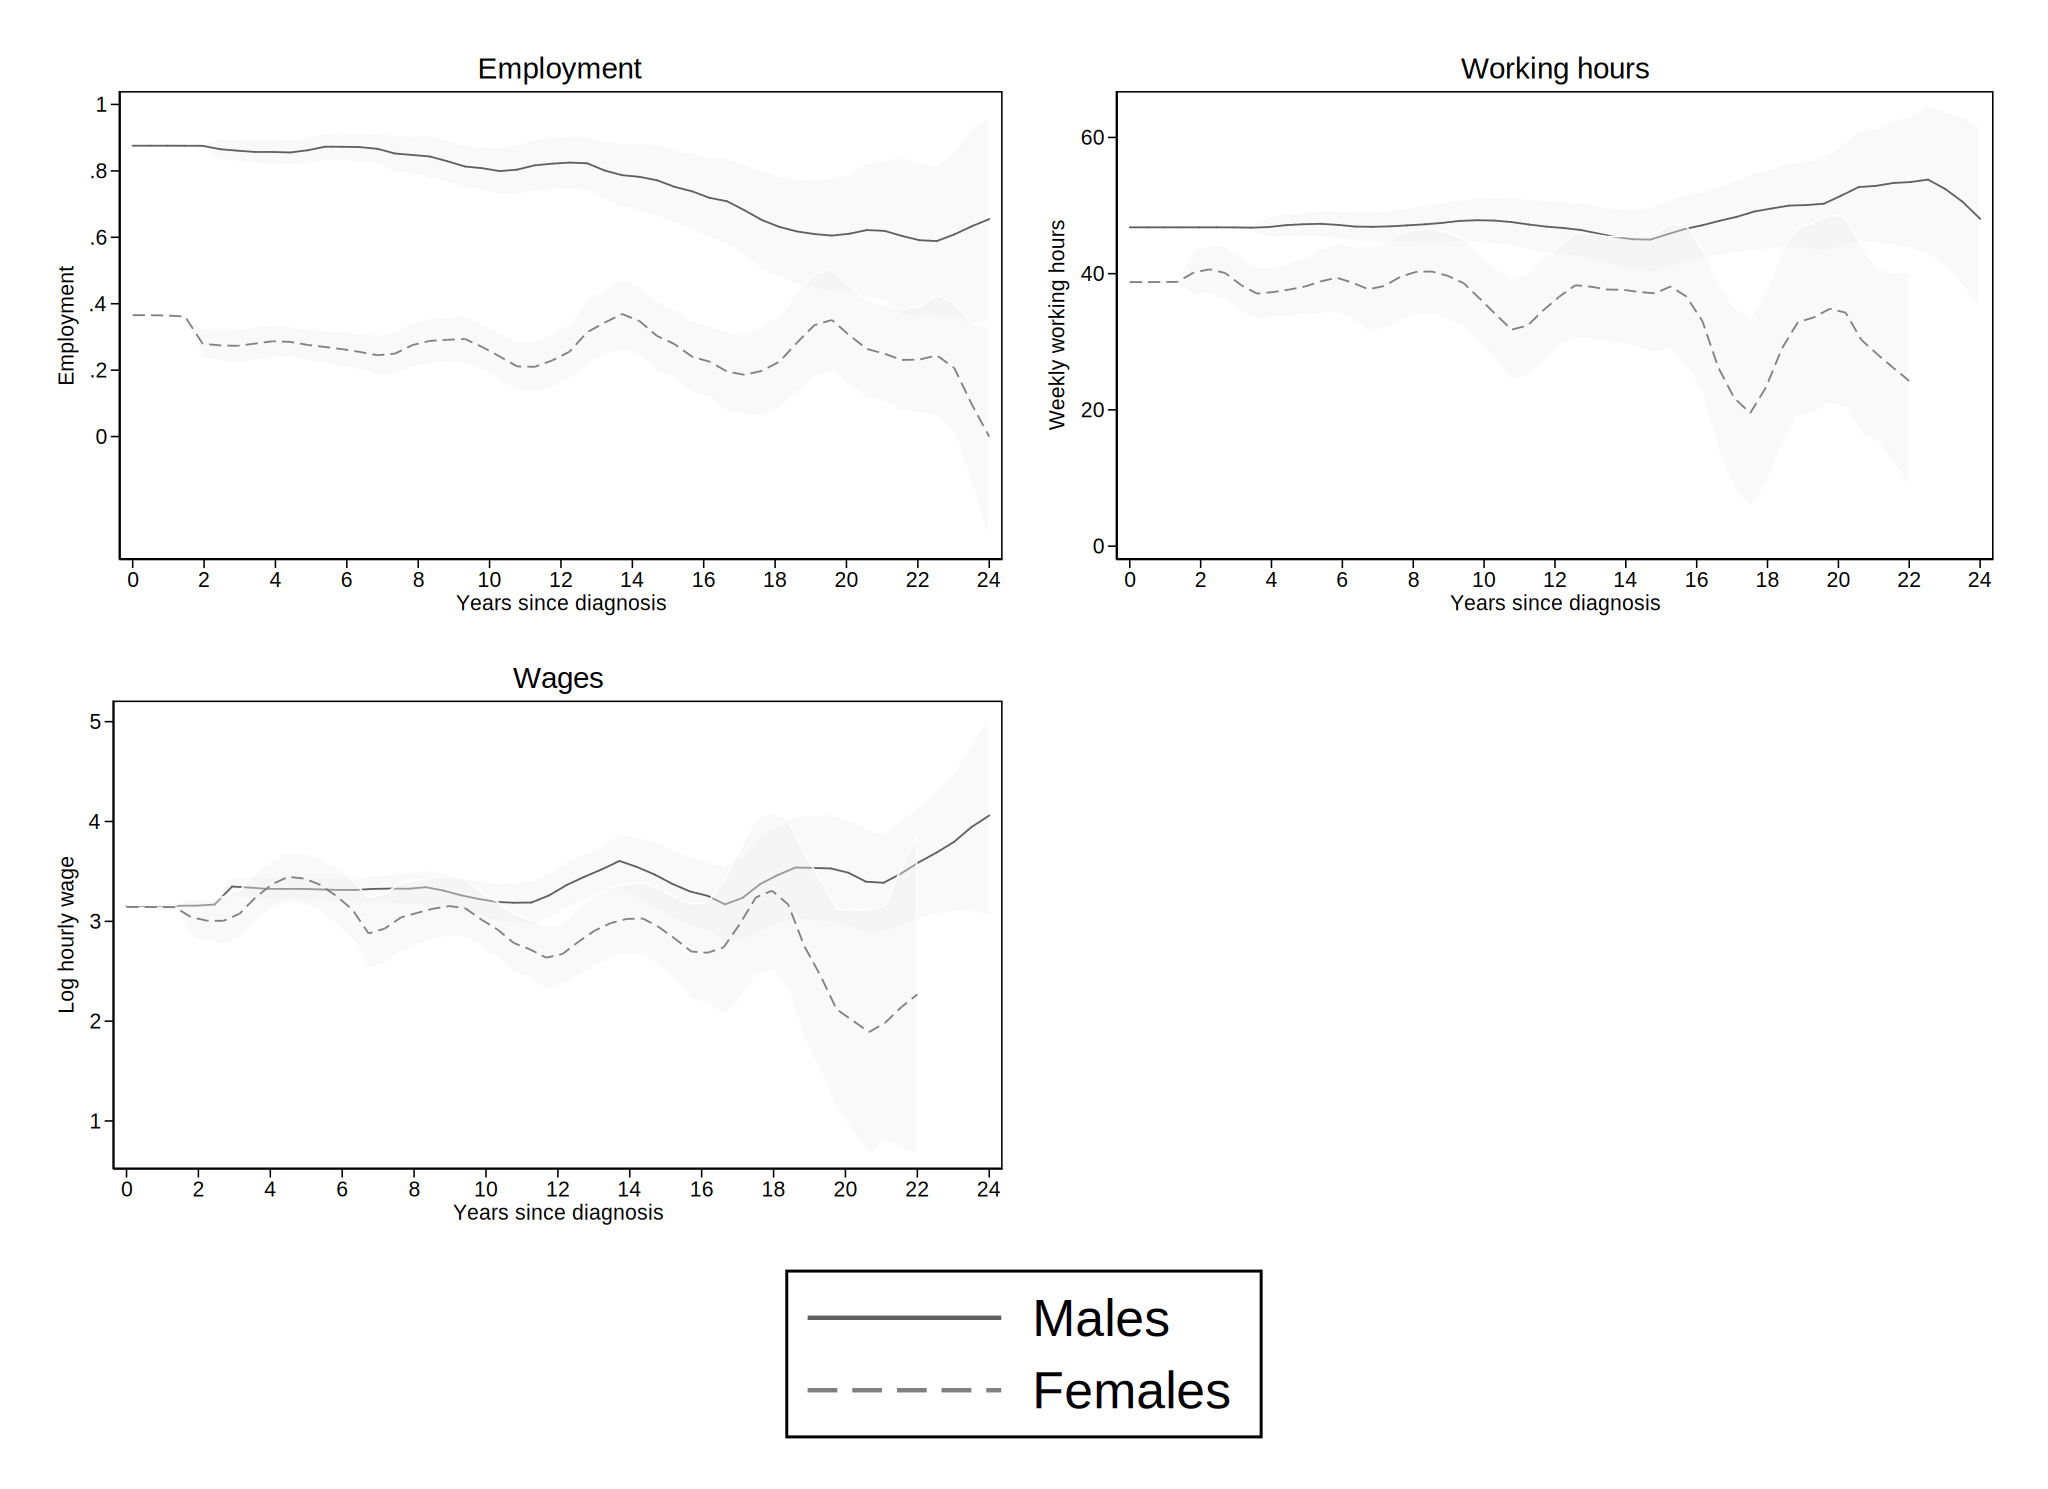
\includegraphics[width=\linewidth]{figures/lpoly_combined.pdf}\\
		\footnotesize{\textit{Notes} The shaded areas indicate the 95\% confidence intervals.}
	\end{center}
\end{figure}



\end{document}

